

\section*{Appendix Overview}

The appendix is organised into six parts that follow the paper's evidence chain. Parts~A--B complete
the method and theory; Part~C fixes the shared experimental protocol; Part~D provides the full result
record; Part~E collects mechanism, ablation and robustness evidence; and Part~F records scope and
reproducibility information. Parts are top-level sections; the heavy ones group their material into
subsections.

\begin{itemize}\itemsep2pt
\item \textbf{\Cref{app:method}, method and algorithmic details.} Notation, the structured-unit and
mask semantics with the physical-removal equivalence test, the estimator and its Gram construction,
the solver with its guards and complexity, and the closed-form compensation the same matrix affords.
\item \textbf{\Cref{app:theory}, theoretical analysis.} The risk geometry that makes pruning purely
second order, the Gram identity and the additivity bound behind the surrogate, the reduction of
diagonal \method to structured Optimal Brain Damage, why the calibrated interaction strength is
small, and the solver's marginal-risk and overshoot guarantees.
\item \textbf{\Cref{app:setup}, experimental setup.} Datasets and splits, models and per-model
configurations, baseline descriptions, the evaluation protocol, and the scope of the suite.
\item \textbf{\Cref{app:results}, complete results.} The per-task record behind every main-text
table, the ratio sweep from $10\%$ to $50\%$, the recovery stage, and efficiency.
\item \textbf{\Cref{app:analysis}, mechanism, ablations, and robustness.} Extended ablations, surrogate fidelity,
the mechanism evidence (edge spectra, bridge units, layer structure), the robustness of the
selection under resampling and independent calibration, and how the method behaves where the edges
carry least signal.
\item \textbf{\Cref{app:discussion}, discussion.} Extended related work, limitations, broader
impact, and the reproducibility checklist.
\end{itemize}

\clearpage

% ======================================================================
\section{Method and Algorithmic Details}
\label{app:method}
\subsection{Notation}

\label{app:notation}
\cref{tab:notation} collects the symbols used throughout the paper.
\begin{table}[htbp]
\centering\footnotesize
\caption{\textbf{Summary of notation.}}
\label{tab:notation}
\setlength{\tabcolsep}{7pt}\renewcommand{\arraystretch}{1.18}
\begin{tabular}{@{}l@{\quad}p{0.70\linewidth}@{}}
\toprule
Symbol & Meaning\\
\midrule
\multicolumn{2}{l}{\emph{Units, masks, and budget}}\\
$\Uset=\{u_1,\dots,u_M\}$ & the $M$ removable structured units (attention heads, FFN channel groups)\\
$s_u$,\, $s$ & pruning variable ($s_u{=}1$ removes unit $u$) and the full mask vector; the deployed
mask is binary, and $s$ is real-valued near $\mathbf 0$ so that \cref{eq:quadratic} is well posed\\
$m_u=1-s_u$ & keep gate scaling unit $u$'s write into the residual stream\\
$c_u=\Param(u)$ & removable parameter cost of unit $u$\\
$\rho$ & target pruning ratio (removed non-embedding parameter fraction)\\
$S$,\, $|S|$ & selected (pruned) unit set and its size; $\mathcal K$: kept FFN groups (compensation)\\
\midrule
\multicolumn{2}{l}{\emph{Curvature matrix (the central object)}}\\
$\Hmat\in\mathbb{R}^{M\times M}$ & co-pruning curvature (Fisher) matrix, as estimated from the $M$
ablations (\cref{eq:gram})\\
$\Hmat^\star=\mathbb{E}[J^\top FJ]$ & the exact curvature $\Hmat$ estimates, with
$J=\partial z_s/\partial s|_{s=\mathbf 0}$ (\cref{rem:exact})\\
$\Hmat_{uu}$ & \textbf{node saliency} (diagonal): an OBD-style importance\\
$\Hmat_{uv}$ & \textbf{co-pruning curvature edge} (off-diagonal): the joint-removal cost of $u$ and $v$\\
$\rho_{uv}\in[-1,1]$ & curvature correlation $\Hmat_{uv}/\sqrt{\Hmat_{uu}\Hmat_{vv}}$; signed, since
cross terms cancel. \Cref{fig:anatomy} reports its magnitude $|\rho_{uv}|$\\

\midrule
\multicolumn{2}{l}{\emph{Objective and estimation}}\\
$\mathcal R(s)$ & pruning risk: token-level KL between teacher and masked model (\cref{eq:risk})\\
$\widehat{\mathcal R}_\lambda(s)$ & the surrogate the solver minimises, $\lambda{=}1$ written
$\widehat{\mathcal R}(s)=\tfrac12 s^\top\Hmat s$ (\cref{eq:objective})\\
$\Delta z_s=z_0-z_s$ & logit perturbation of the masked model, $\approx\sum_u s_u\,\delta z_u$\\
$\Delta R(u\mid S)$,\, $g_u^{(S)}$ & marginal risk of adding $u$ to $S$, and its interaction accumulator
(\cref{eq:marginal})\\
$p_0,z_0$\, / \,$p_s,z_s$ & teacher (frozen) and masked-model next-token distributions / logits\\
$F$ & per-token Fisher $\mathrm{diag}(p_0)-p_0p_0^{\!\top}$ in logit space\\
$\delta z_u$,\, $\widetilde{\delta z}_u$ & single-unit logit perturbation from ablating $u$; its whitened feature ($\Hmat$ is their Gram)\\
$\mathcal C$,\, $\mathcal C'$ & calibration set building $\Hmat$, and the disjoint split $\hat\lambda$ is
measured on (\cref{eq:lambdahat})\\
$r$,\, $n_f$,\, $P$ & top-$r$ logit support, FFN groups per layer, total calibration positions\\
\midrule
\multicolumn{2}{l}{\emph{Solver and compensation}}\\
$\lambda\in[0,1]$,\, $\hat\lambda$ & interaction strength scaling the off-diagonal, and the value
selected on held-out risk (\cref{eq:lambda}, \cref{eq:lambdahat})\\
$\mathcal F=\{S_\lambda\}$,\, $|\mathcal F|$ & the finite family of prunings the path enumerates, and its
size\\
$\kappa$,\, $\mathcal L_p$ & per-layer removed-cost cap and the set of protected layers; one rule,
$\kappa{=}1.5\rho$ with two layers protected at each end (\cref{app:protocol})\\
$\mu_u,\, \nu_u$ & intercept and $\lambda$-slope of the cost-normalised marginal (\cref{eq:affine});
the breakpoints of the path are their crossings\\
$b_u=\sum_{v\ne u}|\Hmat_{uv}|$ & a unit's total coupling; with $\Hmat_{uu}$ it defines the
\emph{bridge} corner (\cref{app:mechanism})\\
$\bar\rho_S$ & the $\sqrt{\Hmat_{uu}\Hmat_{vv}}$-weighted mean of $\rho_{uv}$ over in-set pairs
(\cref{prop:offdiag})\\
$\gamma,\, \tau,\, \alpha$ & compensation ridge strength, clip radius, and rescale coefficients (\cref{eq:comp})\\
\bottomrule
\end{tabular}
\end{table}
\subsection{Structured Units, Mask Semantics, and Physical Pruning}

\label{app:units}

\textbf{Attention units.} For multi-head attention (MHA), one head is one unit; pruning head $i$
removes the corresponding rows of $W_Q,W_K,W_V$ and the input columns of $W_O$. For grouped-query
attention (GQA)~\citep{ainslie2023gqa} with $n_g=n_q/n_{kv}$ query heads per KV head, the unit is the
KV-aligned query-head group $\mathcal{I}_g=\{g r_{\mathrm{kv}},\dots,(g{+}1)r_{\mathrm{kv}}{-}1\}$; pruning group $g$ removes the
rows of $W_Q$ for $i\in\mathcal{I}_g$, the rows of $W_K,W_V$ for KV head $g$, and the matching input
columns of $W_O$. The head dimension $d_h$ is kept fixed (we never re-infer $d_h=d/n_q$ after pruning,
which would corrupt models that derive $d_h$ from the head count); a patched attention module stores
the reduced $n_q',n_{kv}'$ explicitly.

\textbf{FFN groups.} The intermediate dimension is partitioned into $n_f$ contiguous groups. Because
the map from the (gated) intermediate activation to the FFN output is linear, the output is exactly the
sum of per-group contributions, so pruning group $j$ removes the rows of $W_{\text{gate}},W_{\text{up}}$
(or $W_1$) and the columns of $W_{\text{down}}$ (or $W_2$) for that group. The runtime mask zeros the
gated product before the down projection; equivalently it zeros those up/gate rows, since the
SwiGLU/GELU gate satisfies $\sigma(0)\cdot(\cdot)=0$.

\textbf{Mask boundary and equivalence.} A runtime mask zeros only a unit's residual-stream
contribution and never alters normalisation, RoPE, residual addition, causal/padding masks, GQA repeat
rules, or dropout (the model is in eval mode). Two things follow, and we check them
separately. Zeroing a unit's weight slices is bit-identical to masking it at runtime, which we verify
on a held-out batch, so a masked evaluation and a zeroed one are the same measurement. Slicing the
weight matrices instead is what the timings run on, and its correctness is checked by the realised
parameter count of every timed model: on Llama-3.1-8B-Instruct at $\rho{=}20\%$ the sliced model holds
$6.633$B parameters against the dense $8.030$B, and the logit equivalence of the slicing path is
verified on a synthetic grouped-query Llama to $10^{-4}$. Reported speedups therefore come from a
smaller model, not from zeroed weights in a full-size one.
\subsection{The CoCurve Estimator}

\label{app:estimation}

\cref{alg:estimate} details the estimator. The crux (\cref{prop:gram}) is that gathering every unit's
ablated logits on the same teacher top-$r$ support $\mathcal{V}_r(x,t)$ places all single-unit
features in one coordinate system, so $\Hmat$ is a Gram matrix and the off-diagonal edges cost nothing
beyond the $M$ diagonal ablations. We never materialize the $V\times V$ Fisher.

\begin{algorithm}[t]
\caption{\methodfull\ matrix estimation (single-unit, top-$r$ Fisher Gram)}
\label{alg:estimate}
\begin{algorithmic}[1]
\REQUIRE frozen $f_0$, calibration $\mathcal{C}$, units $\Uset$, top-$r$, token budget $P_{\rm tok}$
\STATE \textbf{Teacher pass:} for each $x\in\mathcal{C}$, select token positions $\mathcal{T}(x)$; store
  top-$r$ indices $\mathcal{V}_r(x,t)$ and renormalised probs $p_0$
\FOR{each unit $u\in\Uset$} \COMMENT{$M$ passes; embarrassingly parallel}
  \STATE run $f_{-u}$ (mask only $u$); gather $z_{-u}$ on the teacher support $\mathcal{V}_r(x,t)$
  \STATE $\delta z_u\leftarrow z_0-z_{-u}$;\quad
         $\widetilde{\delta z}_u\leftarrow \sqrt{p_0}\odot(\delta z_u-\mathbb{E}_{p_0}[\delta z_u])$
  \STATE append $\widetilde{\delta z}_u$ to feature store $\bar D_u$ (CPU/memmap)
\ENDFOR
\STATE $\Hmat\leftarrow \tfrac1P\,\bar D^\top\bar D$ (blockwise Gram); $\Hmat\leftarrow\tfrac12(\Hmat+\Hmat^\top)$
\STATE assert $\min_u\Hmat_{uu}\ge -\epsilon$ \COMMENT{non-negativity check (\cref{prop:gram})}
\RETURN $\Hmat$
\end{algorithmic}
\end{algorithm}

\textbf{Top-$r$ coordinate consistency.} Using a per-unit top-$r$ would place different units in
different coordinate systems and invalidate the Gram; the shared teacher support is essential.
Defaults: $r{=}256$, $128$ C4 sequences of length $2048$, deterministic token subsampling
($P_{\rm tok}{=}128$, so $P=16384$ stored positions). Increasing $r$ beyond $256$ leaves $\Hmat$ nearly unchanged (\cref{app:ablation-extra}).

\textbf{Optional prefix-cache replay.} An exact speedup caches residual states before the masked
computation and replays everything after: attention ablations replay from the pre-attention residual,
FFN ablations from the pre-FFN residual. Multiple masks can share an input batch via the batch
dimension. This changes wall-clock, not the estimate.
\subsection{The Greedy Co-Pruning Solver}

\label{app:solver}

\cref{alg:edge-taylor} summarises the full \method pipeline end to end (calibrate, ablate, build the
Gram edge matrix, greedily co-prune, physically remove).
\begin{algorithm}[htbp]
\caption{\methodfull: end-to-end co-pruning pipeline.}
\label{alg:edge-taylor}
\begin{algorithmic}[1]
\REQUIRE frozen model $f_0$, calibration set $\mathcal{C}$, units $\Uset$ with costs $\{c_u\}$, ratio $\rho$,
  interaction strength $\hat\lambda$ (\cref{eq:lambdahat}), per-layer cap $\kappa$, protected layers $\mathcal{L}_p$
\STATE run $f_0$ on $\mathcal{C}$; cache token positions, teacher top-$r$ indices and probabilities
\FOR{each unit $u\in\Uset$}
  \STATE mask only $u$; gather ablated logits on the teacher's top-$r$ indices; form $\widetilde{\delta z}_u$ \hfill // $M$ ablations
\ENDFOR
\STATE $\Hmat\leftarrow \tfrac1P\,\bar D^\top \bar D$; symmetrize $\Hmat\leftarrow\tfrac12(\Hmat+\Hmat^\top)$ \hfill // Gram, \cref{eq:gram}
\STATE $S\leftarrow\emptyset,\;g\leftarrow\mathbf{0},\;C_S\leftarrow0$
\WHILE{$C_S<\rho\sum_u c_u$}
  \STATE $\mathcal{A}\leftarrow\{u\notin S:\ \mathrm{layer}(u)\notin\mathcal{L}_p,\ c_u\text{ fits the layer cap }\kappa\}$;\quad \textbf{if} $\mathcal{A}=\emptyset$ \textbf{then break}
  \STATE $u^\star\leftarrow\arg\min_{u\in\mathcal{A}}\big(\tfrac12\Hmat_{uu}+\hat\lambda\,g_u\big)/c_u$ \hfill // \cref{eq:marginal}
  \STATE $S\leftarrow S\cup\{u^\star\}$;\quad $g\leftarrow g+\Hmat_{:,u^\star}$;\quad $C_S\leftarrow C_S+c_{u^\star}$
\ENDWHILE
\STATE slice the weight matrices of $S$; verify the realised parameter count
\RETURN compressed model $f_S$ and $\rho_{\mathrm{actual}}=C_S/\sum_u c_u$
\end{algorithmic}
\end{algorithm}
\cref{alg:solve} gives the solver. By \cref{prop:greedy}, maintaining the running interaction vector
$g_u=\sum_{v\in S}\Hmat_{uv}$ makes each step $O(M)$. Two guards keep pruning distributed without
changing the objective: a per-layer cost cap and first/last-layer protection. Both are fixed by one
rule, cap $=1.5\rho$ with the first and last two layers protected, applied identically to every
model, every ratio and every method, with no per-model choice and no reference ratio
(\cref{app:protocol}).

\begin{algorithm}[t]
\caption{One-shot cost-normalised greedy co-pruning}
\label{alg:solve}
\begin{algorithmic}[1]
\REQUIRE $\Hmat$, costs $\{c_u\}$, ratio $\rho$, interaction strength $\hat\lambda$, per-layer cap $\kappa$, protected layers $\mathcal{L}_p$
\STATE $S\leftarrow\emptyset$;\; $g\leftarrow\mathbf{0}$;\; $C_S\leftarrow 0$
\WHILE{$C_S<\rho\sum_u c_u$}
  \STATE $\mathcal{A}\leftarrow\{u\notin S:\ \mathrm{layer}(u)\notin\mathcal{L}_p,\ C_{\mathrm{layer}(u)}+c_u\le\kappa\,C^{\rm tot}_{\mathrm{layer}(u)}\}$;\quad \textbf{if} $\mathcal{A}=\emptyset$ \textbf{then break}
  \STATE $u^\star\leftarrow\arg\min_{u\in\mathcal{A}}\big(\tfrac12\Hmat_{uu}+\hat\lambda\,g_u\big)/c_u$
  \STATE $S\leftarrow S\cup\{u^\star\}$;\; $g\leftarrow g+\Hmat_{:,u^\star}$;\; $C_S\leftarrow C_S+c_{u^\star}$
\ENDWHILE
\STATE slice the weight matrices of $S$; verify the realised parameter count
\RETURN $f_S$, $\rho_{\rm actual}=C_S/\sum_u c_u$
\end{algorithmic}
\end{algorithm}

\subsubsection{Complexity and cost}
\label{app:complexity}
Estimation is $M$ forward-only ablation passes over $|\mathcal{C}|$ sequences (no backward pass,
Hessian-vector product, or pairwise ablation); the Gram is $O(M^2 P r)$ multiply-adds, accumulated
blockwise. The solver is $O(M|S|)$ for $|S|$ selected units. With FFN grouping ($M\!\sim\!10^3$) the whole
pipeline is one-shot per (model, ratio) and fits commodity hardware; wall-clock is reported in
\cref{app:efficiency}.

% =====================================================================
\clearpage

% ======================================================================
% ======================================================================
\subsection{Edge-Derived Coupling-Aware Compensation}
\label{app:comp}

Selection alone discards every removed unit's contribution, but the same edge matrix that scored
the interactions tells us how to absorb that lost contribution. Removing $S$ shifts the residual stream by
$\Delta z_S\approx\sum_{u\in S}\delta z_u$; among the kept FFN groups $\mathcal K$ we choose a per-group
output rescale $1+\alpha_v$ that cancels $\Delta z_S$ in the Fisher geometry, minimizing
$\mathbb{E}_{x,t}\big[\big(\textstyle\sum_{v\in\mathcal K}\alpha_v\delta z_v-\Delta z_S\big)^{\!\top} F \big(\textstyle\sum_{v\in\mathcal K}\alpha_v\delta z_v-\Delta z_S\big)\big]+\gamma\|\alpha\|_2^2$
over the coefficient vector $\alpha$. Taking the expectation over positions turns the quadratic and linear terms into blocks of $\Hmat$
itself (\cref{eq:huv}). The normal equations are then a small ridge system in edge blocks we have
already computed,
\begin{equation}
(\Hmat_{\mathcal K\mathcal K}+\gamma I)\,\alpha=\Hmat_{\mathcal K S}\,\mathbf 1_S,
\qquad
\text{gain}_v=\mathrm{clip}(1+\alpha_v,\,1\!-\!\tau,\,1\!+\!\tau),
\label{eq:comp}
\end{equation}
where $\mathbf 1_S$ is the all-ones vector indexed by $S$, and the ridge strength $\gamma$ and clip
radius $\tau$ are the released defaults of \cref{app:protocol}.
This is one $|\mathcal K|\times|\mathcal K|$ CPU solve, with no gradients, no data beyond the calibration
used to build $\Hmat$, and, unlike OBS-style reconstruction, no per-layer weight inverse. No number reported
anywhere in this paper uses it: every result in the main tables and in \cref{tab:ratio-full} is
selection-only, so the comparison stays about which units are removed. We include the derivation
because it is the same matrix used a second way. The couplings that say what \emph{not} to remove
together also say how the survivors should absorb what was removed, and because it
costs one small ridge solve rather than the per-layer weight inverse that OBS-style reconstruction
needs.

\section{Theoretical Analysis}
\label{app:theory}

% =====================================================================
We collect the formal results behind \cref{sec:method} and, for each, state how it is validated
empirically. Notation: $p_0$ is the teacher distribution, $z_0$ its logits,
$F=\mathrm{diag}(p_0)-p_0p_0^\top$ the KL Fisher, and $\delta z_u=z_0-z_{-u}$ the single-unit logit
perturbation. We use local additivity $z_0-z_s\approx\sum_u s_u\delta z_u$, ; \cref{prop:additivity} bounds the third-order
remainder of the exact quadratic, and the additivity substitution itself is measured rather than
bounded (\cref{app:th-est}).
\subsection{Geometry of the Pruning Risk}

\label{app:th-geom}
\paragraph{Why pruning is purely second order.}
\begin{proposition}[Vanishing zeroth/first order]\label{prop:vanish}
With $s$ ranging over a neighbourhood of $\mathbf 0$ in $\mathbb{R}^M$ (\cref{sec:method}), so that
$\mathbf 0$ is interior and $\mathcal{R}$ is differentiable there,
$\mathcal{R}(\mathbf 0)=0$ and $\nabla_s\mathcal{R}(\mathbf 0)=0$; the Taylor expansion at the full model
begins at second order.
\end{proposition}
\begin{proof}
At $s=\mathbf 0$, $p_{\mathbf 0}=p_0$, so every term is $\KL(p_0\|p_0)=0$. For the gradient, with
$g(s)=\KL(p_0\|p_s)$ and $p_s$ a softmax,
$\partial_{s_u}g=-\mathbb{E}_{p_0}[\partial_{s_u}z_s]+\mathbb{E}_{p_s}[\partial_{s_u}z_s]$; at
$s=\mathbf 0$, $p_s=p_0$ and the two expectations cancel. Averaging over positions preserves equality.
\end{proof}
\noindent\emph{Significance.} The absence of a first-order term is what makes the off-diagonal
curvature, not a gradient, the carrier of interaction information; it also means saliency itself
is second order, unifying our diagonal with classical second-order pruning.

\begin{proposition}[Fisher quadratic]\label{prop:fisher}
To second order, $\KL(p_0\|p_s)\approx\tfrac12\,\Delta z_s^\top F\,\Delta z_s$ with
$\Delta z_s=z_0-z_s$; hence under local additivity
$\Hmat_{uv}=\mathbb{E}_{x,t}[\delta z_u^\top F\,\delta z_v]$ (\cref{eq:huv}).
\end{proposition}
\begin{proof}
For $A(z)=\log\sum_y e^{z_y}$ we have $\nabla A=p_0$ and $\nabla^2A=F$ at $z_0$. Writing
$\Delta=\Delta z_s=z_0-z_s$, so that $z_s=z_0-\Delta$,
$A(z_0{-}\Delta)=A(z_0)-p_0^\top\Delta+\tfrac12\Delta^\top F\Delta+o(\|\Delta\|^2)$. Since
$\KL(p_0\|p_s)=-p_0^\top(z_s-z_0)+A(z_s)-A(z_0)=p_0^\top\Delta+A(z_0{-}\Delta)-A(z_0)$, the linear terms
cancel and $\KL(p_0\|p_s)=\tfrac12\Delta^\top F\Delta+o(\|\Delta\|^2)$. Local additivity gives
$\Delta z_s\approx\sum_u s_u\,\delta z_u$ with $\delta z_u=z_0-z_{-u}$; substituting and taking
expectations gives the matrix.
\end{proof}
\subsection{Tractable Estimation}

\label{app:th-est}
\paragraph{The full edge matrix from $M$ ablations.}
\begin{proposition}[Gram equivalence]\label{prop:gram}
With $\widetilde{\delta z}_u=\sqrt{p_0}\odot(\delta z_u-\mathbb{E}_{p_0}[\delta z_u])$,
$\delta z_u^\top F\delta z_v=\widetilde{\delta z}_u^\top\widetilde{\delta z}_v$. Hence
$\Hmat=\tfrac1P\bar D^\top\bar D\succeq0$, where $\bar D$ has columns $\bar D_u$, with
$\Hmat_{uu}=\tfrac1P\|\bar D_u\|^2\ge0$, recoverable from $M$ single-unit ablations with no pairwise
computation.
\end{proposition}
\begin{proof}
$a^\top Fb=\sum_y p_{0,y}a_yb_y-(\sum_y p_{0,y}a_y)(\sum_y p_{0,y}b_y)=\sum_y p_{0,y}(a_y-\bar a)(b_y-\bar b)
=(\sqrt{p_0}\odot(a-\bar a))^\top(\sqrt{p_0}\odot(b-\bar b))$. Set $a=\delta z_u,b=\delta z_v$; stack over
positions to get the Gram, which is PSD with non-negative diagonal.
\end{proof}
\noindent\emph{Significance.} A model with $O(M^2)$ edges costs only $O(M)$ ablations
because each edge is an inner product of two single-unit features. This is what makes edge-aware
structured pruning practical, and the symmetrisation and non-negative-diagonal steps of \cref{alg:estimate} are guards on float accumulation, not conditions the estimator could fail: \cref{prop:gram} gives both exactly.

\paragraph{Exact curvature vs.\ the estimator we use.} It is worth separating what is exact from what
is approximated, since our claims rest only on the former being a good surrogate, not on equality.
\begin{remark}[What is exact, what is a surrogate]\label{rem:exact}
Two statements are exact (to the stated order): (a) the KL between teacher and masked model is
the Fisher-weighted logit norm to second order,
$\KL(p_0\|p_s)=\tfrac12\Delta z_s^\top F\Delta z_s+o(\|\Delta z_s\|^2)$ (\cref{prop:fisher}); and (b) the Gram identity
$\delta z_u^\top F\,\delta z_v=\widetilde{\delta z}_u^\top\widetilde{\delta z}_v$ (\cref{prop:gram}).
What we estimate rather than compute exactly is the curvature matrix itself. The exact Hessian, which
here coincides with the Gauss--Newton matrix because the logit-space gradient vanishes at
$s=\mathbf 0$ (\cref{prop:vanish}), is $\Hmat^\star=\mathbb{E}[J^\top F J]$ with $J=\partial z_s/\partial s|_{s=0}$;
we replace the infinitesimal column $J_u$ by the finite single-unit ablation
$\delta z_u=z_0-z_{-u}$, and we take $F$ from the teacher's top-$r$ support renormalised to sum to one,
so $F$ throughout is the Fisher of that truncated distribution rather than of the full vocabulary.
Hence our $\Hmat$ is a finite-difference, renormalised top-$r$ Fisher-Gram surrogate for
$\Hmat^\star$, exact in the linear-network, infinitesimal-mask, full-vocabulary limit and an empirical
proxy otherwise. The truncation behaves the same way at both ends of our
scale range: at $r{=}256$ the retained teacher mass has median $0.993$ on Llama-3.2-3B and $0.992$ on
Mistral-Small-24B, over $16{,}384$ sampled calibration positions each. The tail is worth stating
rather than hiding --- the fifth percentile is $0.90$ and $0.87$, the first $0.77$ and $0.71$, and
about two positions in five retain under $0.99$ --- because the claim that carries weight is not that
every position is covered but that the estimator does not depend on how much of the tail is kept, and
that is measured directly: $r$ over a fourfold range moves nothing (\cref{tab:sensitivity}). What we rely on is $\Hmat$ ranking co-pruning damage,
which we validate directly (\cref{app:surrogate}, \cref{sec:exp-analysis}).
\end{remark}

\paragraph{Three approximations, separated and measured.}
Three distinct steps separate the token-level KL from the quadratic the solver minimises. Only the
first is asymptotic in $\|s\|$; the other two are fixed properties of the estimator, which is why we
measure them rather than bound them.

\begin{proposition}[Third-order remainder]\label{prop:additivity}
Let $\Hmat^\star=\mathbb{E}[J^\top F J]$ with $J=\partial z_s/\partial s|_{s=\mathbf 0}$ be the exact
Gauss--Newton curvature of \cref{eq:risk}. If the logit map is twice differentiable in the mask
variables near $s=\mathbf 0$ with second derivatives bounded on $\|s\|_1\le\delta$, then there is a
constant $C$, depending on that bound and not on $s$, with
$\big|\mathcal{R}(s)-\tfrac12 s^\top\Hmat^\star s\big|\le C\|s\|_1^3$ for all $\|s\|_1\le\delta$.
\end{proposition}
\noindent The masks we deploy are binary with $\|s\|_1=|S|$ in the hundreds, well outside any radius
on which this is a useful numerical bound. It is stated because it identifies \emph{which} term is
missing --- third order in the mask, not the two estimator steps below --- and the size of that term at
the ratios we prune is settled by measurement, not by the constant.
\begin{proof}[Proof sketch]
The KL expansion of \cref{prop:fisher} drops an $o(\|\Delta\|^2)$ term whose leading part is the cubic
log-partition derivative, $O(\|\Delta\|^3)$ with $\Delta=\Delta z_s$; smoothness bounds $\|\Delta\|$ by
$O(\|s\|_1)$. The same smoothness makes $\Delta z_s=Js+O(\|s\|_1^2)$, whose cross term with the
quadratic contributes at the same cubic order.
\end{proof}

\noindent This bounds $\Hmat^\star$, the exact curvature. Two further steps carry us from
$\Hmat^\star$ to the matrix we build, and we measure both.

\textbf{(i) Finite ablation in place of the derivative column.} We replace $J_u$ by
$\delta z_u=z_0-z_{-u}$, a secant over the whole mask interval rather than a tangent. Scaling a unit's
residual contribution by $1-\epsilon$ and forming $\delta z_u^{(\epsilon)}=(z_0-z_{u,\epsilon})/\epsilon$
for $\epsilon\in\{1,\tfrac12,\tfrac14,\tfrac18\}$ lets us compare the two directly. On a stratified
sample of units the hard ablation recovers the derivative direction to a median cosine of
$0.949$--$0.981$ across four models, with $\|\delta z_u\|/\|J_u\|=1.03$--$1.07$: the secant is the
tangent to within a few degrees and a few percent. This comparison requires fp32: in bf16 the small-$\epsilon$ difference falls to the logit noise
floor and the $\epsilon$-ladder no longer resolves.

\textbf{(ii) Local additivity.} The off-diagonal additionally assumes
$\Delta z_S\approx\sum_{u\in S}\delta z_u$. Comparing the predicted quadratic
$\tfrac12\,\mathbb{E}_{x,t}\|\sum_{u\in S}\widetilde{\delta z}_u\|^2$ (which is exactly
$\tfrac12 s^\top\Hmat s$ by \cref{prop:gram}) against the same form evaluated on the true joint
perturbation, $\tfrac12\,\mathbb{E}_{x,t}\|\widetilde{\delta z}_S\|^2$ with
$\widetilde{\delta z}_S=\sqrt{p_0}\odot(\Delta z_S-\mathbb{E}_{p_0}[\Delta z_S])$, isolates this
step. The additive reconstruction drifts in
\emph{direction} as the set grows (cosine $0.997\!\to\!0.53$ from $|S|=2$ to $\rho=25\%$), but the
quadratic \emph{value} is preserved throughout, the ratio staying in $0.67$--$1.18$. Both diagnostics
rebuild the features in fp32 on eight held-out sequences of
$512$ tokens, because the $\epsilon$-ladder of (i) does not resolve in bf16; they therefore isolate the
two substitutions rather than characterising the shipped matrix, which is accumulated in bf16 over
$128$ sequences of $2048$.

\noindent\emph{What this calibrates, and what it does not.} Both substitutions leave the quadratic's
\emph{value} stable across $\rho$, so neither is what degrades with the budget; what grows with $\rho$ is
the third-order term in the mask, the one \cref{prop:additivity} names and the one no second-order
surrogate carries. Neither substitution, however, calibrates the surrogate in nats. On the deployed
Llama-3.1-8B-Instruct mask at $\rho{=}20\%$, $\tfrac12 s^\top\Hmat s=7.21$ against a measured held-out
risk of $0.57$: the surrogate over-predicts the absolute KL by about an order of magnitude, and by a
near-uniform factor across ratios. This is immaterial to the use we put it to. By \cref{lem:scale} the
solver reads $\Hmat$ only up to a positive scalar, and $\hat\lambda$ is selected on measured risk rather
than on the surrogate's value, so no positive rescaling --- from the bf16 accumulation, the top-$r$
renormalisation or the finite ablation --- can move a single selection. What the surrogate must do is
\emph{rank} prunings at a fixed budget, and that is measured directly in \cref{app:surrogate}.

\noindent What makes the surrogate an object one can select over is therefore the measurement, not the
remainder, and it is validated directly in \cref{app:surrogate}: predicted surrogate
risk and measured post-pruning KL correlate strongly at low-to-moderate $\rho$ and diverge as $\rho$
grows, matching the cubic gap.
\subsection{Connection to Classical Pruning}

\label{app:classical}
\begin{remark}[Diagonal \method is the structured KL-Fisher analogue of OBD]\label{prop:obd}
Dropping off-diagonals from the implemented surrogate reduces it to $\tfrac12\sum_u\Hmat_{uu}s_u$ with
$\Hmat_{uu}=\mathbb{E}[\delta z_u^\top F\delta z_u]\ge0$, which is an Optimal-Brain-Damage saliency
\citep{lecun1989obd} with structured units in place of weights and a self-distillation KL Fisher in
place of the training-loss Hessian; the first-order term vanishes here exactly at $s=\mathbf 0$
(\cref{prop:vanish}) rather than by an assumption of convergence. \method adds the signed cross-module
curvature $\Hmat_{uv}$, which the diagonal cannot express.
\end{remark}
\noindent\emph{Significance.} This places \method on a continuum with classical second-order pruning:
$\lambda{=}0$ is structured OBD and $\lambda{=}1$ is the full edge model, so the path of
\cref{tab:ablation} measures, at every point, exactly the value added by edges over the classical
baseline.

\paragraph{What a diagonal (cross-term-dropping) method omits.} We can quantify exactly the error that a
diagonal saliency, or any method that discards the off-diagonal terms as higher-order negligible,
incurs relative to the second-order surrogate
$\tfrac12 s^\top\Hmat s$ that both are approximations of (\cref{rem:exact} separates that surrogate
from the true risk).
\begin{proposition}[The diagonal omission is the off-diagonal co-pruning mass]\label{prop:offdiag}
For any pruning set $S$ with indicator mask $s_S\in\{0,1\}^{M}$ ($s_{S,u}{=}1$ iff $u\in S$), the
second-order co-pruning risk and its diagonal (OBD) approximation differ by exactly the off-diagonal
mass of $\Hmat$ on $S$:
\[
\Delta_{\rm off}(S)\;:=\;\underbrace{\tfrac12 s_S^\top\Hmat\,s_S}_{\text{full (\method)}}-\underbrace{\tfrac12\sum_{u\in S}\Hmat_{uu}}_{\text{diagonal (OBD)}}
\;=\;\tfrac12\!\!\sum_{\substack{u,v\in S\\ u\neq v}}\!\!\Hmat_{uv}
\;=\;\tfrac12\!\!\sum_{\substack{u,v\in S\\ u\neq v}}\!\!\rho_{uv}\sqrt{\Hmat_{uu}\Hmat_{vv}},
\]
with $\rho_{uv}=\Hmat_{uv}/\sqrt{\Hmat_{uu}\Hmat_{vv}}$. Consequently, writing
$\bar\rho_S$ for the $\sqrt{\Hmat_{uu}\Hmat_{vv}}$-weighted mean of $\rho_{uv}$ over off-diagonal
pairs in $S$,
$\Delta_{\rm off}(S)=\tfrac12\,\bar\rho_S\big[(\sum_{u\in S}\!\sqrt{\Hmat_{uu}})^2-\sum_{u\in S}\Hmat_{uu}\big]$.
\end{proposition}
\noindent\emph{Significance.} The error of dropping the cross terms is not a vanishing higher-order
remainder. It is a second-order quantity of the same order as the diagonal itself, scaled by the
mean off-diagonal correlation $\bar\rho_S$. It also explains the
\cref{tab:ablation} gap between $\lambda{=}0$ and $\hat\lambda$: the off-diagonal
mass the diagonal ignores is what re-ranks bridge units onto the keep list.

\subsubsection{Selecting the Interaction Strength}
\label{app:lambda}
\emph{This section reports the enumeration, the protocol and the per-model outcome of the path
construction of \cref{sec:method-lambda}.}

\textbf{Why $\lambda$ is not fitted.} The obvious criterion is to choose $\lambda$ so that
$\widehat{\mathcal R}_\lambda$ best matches the risk we measure. It optimises the wrong thing, because the
solver never reads the value of $\widehat{\mathcal R}_\lambda$ --- only the order it induces over candidates,
and that order is invariant to the units $\widehat{\mathcal R}_\lambda$ is expressed in.
\begin{lemma}[Selection is scale-invariant]\label{lem:scale}
For any $a>0$, $\arg\min_{u}\,a\,\Delta R(u\mid S)/c_u=\arg\min_{u}\,\Delta R(u\mid S)/c_u$, where
$\Delta R(u\mid S)$ is the marginal risk of \cref{eq:marginal}.
\end{lemma}
\noindent So a criterion may fit the magnitude of $\widehat{\mathcal R}_\lambda$ perfectly and still select
badly, and it does: magnitude matching returns $\lambda\approx0.1$--$0.4$ on Llama-3.2-3B, and the
pruning it produces is clearly worse than the one \cref{eq:lambdahat} selects. Minimising the risk of
the selections themselves is the criterion that matches what the solver consumes.

\textbf{The family is small, and a sweep does not find it.} Enumerating the breakpoints exactly
(\cref{sec:method-lambda}) yields a few hundred distinct prunings per model over the whole of
$[0,1]$: $288$ on Llama-3.2-3B, $303$ on Llama-3.1-8B-Instruct, $181$ on Falcon3-7B, $400$ on
Yi-1.5-9B. The intervals are narrow and very unevenly sized (Llama-3.2-3B: minimum
$5.6\times10^{-6}$, median $1.8\times10^{-3}$, maximum $0.061$), which is why sampling $\lambda$ is
not an adequate substitute. A sweep at step $0.002$ costs $501$ solves and still reaches only $199$
of the $288$ members, missing $31\%$ of the family and with it the minimum. The miss rate is set by how
unevenly the breakpoints fall rather than by the step size alone: the same sweep misses $13\%$ on
Falcon3-7B and $57\%$ on Yi-1.5-9B, so no step size fixes it across models. The two costs are in different currencies and the walk is not
uniformly cheaper: on Llama-3.2-3B it spends roughly $3\times10^{3}$ CPU greedy solves against the
sweep's $501$, and $288$ masked forward passes against the sweep's $199$. Forward passes dominate the
wall clock, so the walk costs about $1.4\times$ the sweep --- and returns the whole family instead of
$69\%$ of it. Completeness is what is being bought, not speed.

\textbf{The criterion is stable to the calibration split.} $\lambda$ moves the attention/FFN split
of the removed set substantially --- on Llama-3.1-8B-Instruct attention falls from $38\%$ of removed
units at $\lambda\!=\!0$ to $2\%$ at $\lambda\!=\!1$ --- so it is worth asking how much the split
$\mathcal{C}'$ the criterion is measured on decides the answer. Over both context lengths and both
corpora, at $\rho{=}20\%$ with everything else fixed:

\begin{center}
% generated by scripts/make_lambda_protocol_table.py -- do not edit by hand
\footnotesize\setlength{\tabcolsep}{7pt}
\begin{tabular}{@{}ll rr@{}}
\toprule
$\mathcal{C}'$ length & $\mathcal{C}'$ corpus & $\hat\lambda$ & $J$ vs deployed\\
\midrule
$1024$ & C4 & $0.0120$ & $0.967$\\
$1024$ & WikiText & $0.0040$ & $0.877$\\
$\mathbf{2048}$ & \textbf{C4} & $\mathbf{0.0108}$ & \emph{deployed}\\
$2048$ & WikiText & $0.0213$ & $0.844$\\
\bottomrule
\end{tabular}

\end{center}

\noindent $\hat\lambda$ spans $5.3\times$ across the four splits, and the prunings they select agree
with the deployed one at Jaccard $0.84$ to $0.97$. The criterion returns the same pruning whichever
split it is measured on, so we measure it at the deployment context length because that is the risk
the pruned model will incur, not because the number moves: at fixed corpus, doubling the length moves
$\hat\lambda$ by $11\%$.

\Cref{fig:lambdapath} shows the path itself on four models. \textbf{The path on ten models.} The two studies in this paper have different costs, and that is what
sets their breadth. The path needs $\Hmat$ and a held-out set and nothing else, so we report it on all
ten models we estimate $\Hmat$ for. The cross-model comparison additionally needs every baseline
re-selected under the shared guard and re-scored on the full suite --- eight methods, five ratios,
twelve tasks per model --- and we ran that for the five of \cref{tab:cross-model}; on the other five no
baseline has been run under this harness, so no comparison is available on them either way.
\Cref{tab:ablation} applies the protocol unchanged across families and scales. Two patterns hold across them. First, at this ratio $\hat\lambda$ is small on every model, at most
$0.22$ and below $0.05$ on eight of the ten, so the edge term wants to be damped hard. It stays small
at the other ratios too, including on the model whose path was the one apparent exception: on
Mistral-Small-24B the criterion returns $0.034$, $0.044$, $0.043$ and $0.073$ at
$\rho{=}20$, $30$, $40$ and $50\%$. The one point above that scale anywhere in this paper is
$\rho{=}10\%$ on the same model, where it returns $0.71$. We report it and do not explain it: the
$1/(2|S|\bar\rho_S)$ scale would predict roughly a factor of two between $\rho{=}10\%$ and $20\%$ and
the observed ratio is twenty, so whatever moves it is not the size of the removed set alone. It is
also the least consequential ratio in the sweep --- at $\rho{=}10\%$ that model still holds $96.7\%$
of its dense twelve-task average --- and the mask it selects there leads on every column it is
compared on. Second, and much more sharply, $\lambda\!=\!1$ is rejected on \emph{every} model, by $6.7\%$ to
$747\%$ and at $3.8$ to $39.1$ paired standard errors. The minimum is interior on eight of ten, with a margin over $\lambda\!=\!0$
of at least two paired standard errors on seven. On Qwen2.5-7B and Qwen2.5-14B the selected segment
begins at exactly $\lambda\!=\!0$: the protocol declines the edges and returns the diagonal selector.
That is the property that makes $\hat\lambda$ safe to apply without knowing in advance whether a
model's edges are informative.


\begin{figure}[htbp]
\centering
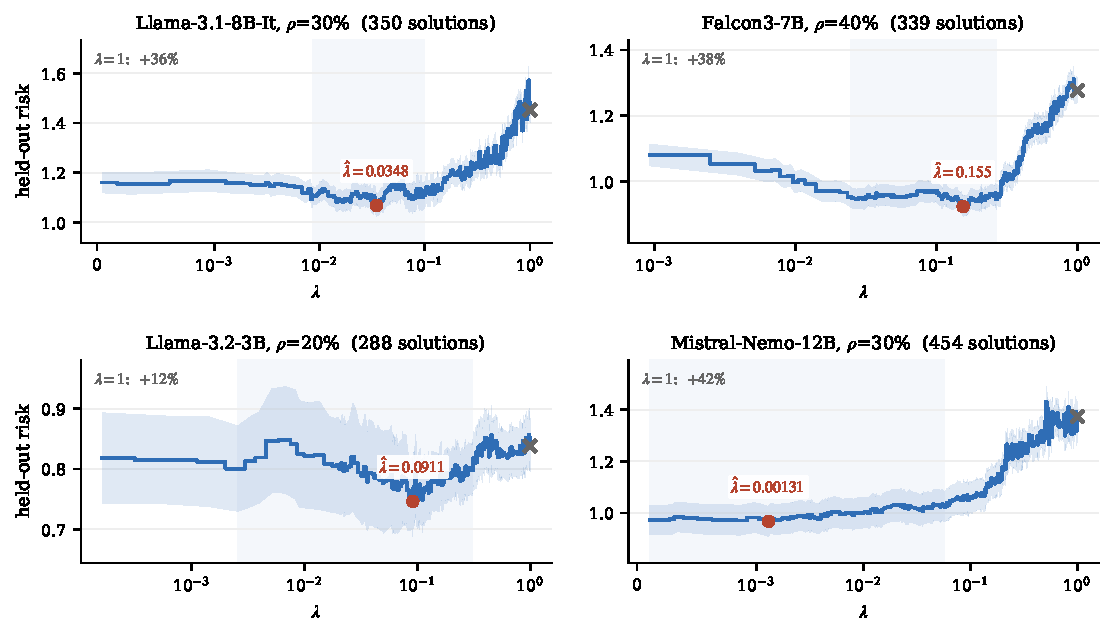
\includegraphics[width=\textwidth]{figures/fig_lambda_path.pdf}
\caption{\textbf{The regularisation path.} Held-out risk against $\lambda$ on four models. The curve
is a step function, since the solution changes only at breakpoints, with the selected point in red,
its $1$-SE band shaded, and the risk at $\lambda{=}1$ marked. The minimum is interior and
$\lambda{=}1$ is far above it everywhere.}
\label{fig:lambdapath}
\end{figure}


\subsubsection{Stability of the estimated matrix}
\label{app:diagnostics}

We rebuild $\Hmat$ independently on random halves of the calibration set, resampling over
\emph{sequences} (positions within a sequence are strongly dependent, so treating the stored positions
as i.i.d.\ would understate the error). Across ten models spanning six families and $3$B--$14$B the
off-diagonal entries reproduce across halves at Pearson $0.885$--$0.996$ and the diagonal at
$0.994$--$1.000$ (\cref{tab:stability}). The edges are estimated, not noise. The finite-ablation
substitution and the additivity step behind them are measured in \cref{app:th-est}.

\begin{table}[htbp]
\centering\footnotesize
\caption{\textbf{Split-half stability of $\Hmat$}, resampled over calibration sequences, mean of four
random halvings. $\mathrm{Jac}(\lambda)$ is the Jaccard overlap of the two independently estimated $20\%$
selections. The edges reproduce nearly as well as the diagonal on every model.}
\label{tab:stability}
% generated by scripts/make_stability_table.py -- do not edit by hand
% 10 models, 4 random halvings each, from outputs/diagnostics/edge_stability/
\setlength{\tabcolsep}{6pt}\renewcommand{\arraystretch}{1.05}
\begin{tabular}{@{}l cc cc@{}}
\toprule
Model & diagonal (Pearson) & \textbf{off-diagonal (Pearson)} & $\mathrm{Jac}(\lambda{=}0)$ & $\mathrm{Jac}(\lambda{=}1)$\\
\midrule
Llama-3.2-3B & 0.996 & 0.885 & 0.661 & 0.569\\
Falcon3-7B & 0.998 & 0.979 & 0.919 & 0.582\\
Mistral-7B & 1.000 & 0.962 & 0.764 & 0.418\\
Qwen2.5-7B & 1.000 & 0.991 & 0.819 & 0.362\\
Llama-3.1-8B-It & 0.994 & 0.905 & 0.672 & 0.509\\
Yi-1.5-9B & 1.000 & 0.966 & 0.853 & 0.729\\
Falcon3-10B & 0.997 & 0.965 & 0.920 & 0.596\\
Mistral-Nemo-12B & 0.999 & 0.982 & 0.598 & 0.456\\
Llama-2-13B & 1.000 & \textbf{0.996} & 0.666 & 0.585\\
Qwen2.5-14B & 0.999 & 0.950 & 0.661 & 0.455\\
\bottomrule
\end{tabular}

\end{table}

\begin{table}[htbp]
\centering\footnotesize
\caption{\textbf{Depth is invisible to the diagonal and monotone in the off-diagonal.} Spearman rank
correlation between a unit's layer index $\ell_u$ and its own saliency $\Hmat_{uu}$, and between
$\ell_u$ and its total coupling $b_u=\sum_{v\neq u}|\Hmat_{uv}|$. One $\Hmat$ per model, the same
build \cref{tab:stability} measures. Coupling is negative on all ten; the saliency column changes
sign across models.}
\label{tab:depth-grading}
% generated by scripts/make_depthgrading_table.py -- do not edit by hand
\footnotesize\setlength{\tabcolsep}{5pt}\renewcommand{\arraystretch}{1.02}
\begin{tabular}{@{}l c rr@{}}
\toprule
Model & $L$ & $\rho_s(\ell_u, \Hmat_{uu})$ & $\rho_s(\ell_u, b_u)$\\
\midrule
Llama-3.2-3B & 28 & $-0.082$ & $\mathbf{-0.874}$\\
Falcon3-7B & 28 & $+0.143$ & $\mathbf{-0.543}$\\
Mistral-7B & 32 & $+0.107$ & $\mathbf{-0.880}$\\
Qwen2.5-7B & 28 & $-0.115$ & $\mathbf{-0.878}$\\
Llama-3.1-8B-It & 32 & $-0.229$ & $\mathbf{-0.867}$\\
Yi-1.5-9B & 48 & $+0.331$ & $\mathbf{-0.806}$\\
Falcon3-10B & 40 & $+0.031$ & $\mathbf{-0.745}$\\
Mistral-Nemo-12B & 40 & $-0.225$ & $\mathbf{-0.910}$\\
Llama-2-13B & 40 & $-0.384$ & $\mathbf{-0.884}$\\
Qwen2.5-14B & 48 & $+0.403$ & $\mathbf{-0.821}$\\
\midrule
\multicolumn{2}{@{}l}{median $|\rho_s|$} & $0.184$ & $\mathbf{0.871}$\\
\bottomrule
\end{tabular}

\end{table}

\subsection{Solver Guarantees}

\label{app:th-solver}
\begin{proposition}[Running-sum marginal]\label{prop:greedy}
$\Delta_\lambda(u\mid S)=\tfrac12\Hmat_{uu}+\lambda g_u$ with $g_u=\sum_{v\in S}\Hmat_{uv}$;
maintaining $g$ by $g\leftarrow g+\Hmat_{:,u^\star}$ makes each step $O(M)$ and the solver $O(M|S|)$,
for any fixed $\lambda$.
\end{proposition}
\begin{proof}
$\widehat{\mathcal R}_\lambda(S)=\tfrac12\sum_{u\in S}\Hmat_{uu}+\lambda\sum_{u<v\in S}\Hmat_{uv}$;
adding $u$ contributes $\tfrac12\Hmat_{uu}+\lambda\sum_{v\in S}\Hmat_{uv}$. The vector $g$ stores
exactly that sum and is updated by one column per selection, independently of $\lambda$.
\end{proof}
\begin{proposition}[Overshoot bound]\label{prop:overshoot}
The stopping rule yields $\rho_{\rm actual}-\rho\le \max_u c_u/\sum_u c_u$.
\end{proposition}
\begin{proof}
Before stopping, $C_{S^-}<\rho\sum_u c_u$; one unit of cost $\le\max_u c_u$ is added, so
$C_S<\rho\sum_u c_u+\max_u c_u$. Divide by $\sum_u c_u$.
\end{proof}
\noindent\emph{Remark (cost-normalised selection).} Choosing $u$ by $\Delta R(u\mid S)/c_u$ is the
density-ordering heuristic for the underlying min-quadratic knapsack, the standard surrogate when an
exact solve is intractable, and the shared budget lets the attention-vs-FFN split emerge from the
objective rather than a hand-set ratio. Density ordering is the right ordering while the marginals are
non-negative, which holds in every run we inspect: $\Hmat_{uu}\ge0$ exactly (\cref{prop:gram}) and all
$11{,}325$ in-set edges are positive on Llama-3.1-8B-Instruct at $\rho{=}20\%$. On a model with
sign-mixed edges a negative marginal should be ordered by $\Delta$ rather than by $\Delta/c_u$, since
dividing a negative gain by cost prefers the cheaper unit.

% =====================================================================
\clearpage

% ======================================================================
\section{Experimental Setup}
\label{app:setup}
\subsection{Datasets}

\label{app:datasets}
\cref{tab:datasets} lists all evaluation benchmarks with task type, metric, and split. Calibration is
$128$ C4 sequences (length $2048$); no task labels are used for pruning. Every method is evaluated on
this same fixed suite and on nothing outside it.

\begin{table}[htbp]
\centering\caption{\textbf{Evaluation suite.} Every multiple-choice task is scored on its full split
through one shared harness; $n$ is the number of items actually scored, and for the perplexity corpora
the number of target tokens under the headline model's tokenizer (the token count, not the corpus,
varies across tokenizers). Multiple choice is length-normalised log-likelihood over the candidate
answers, zero-shot. The capability groups are the ones \cref{tab:cross-model} averages
over.}\label{tab:datasets}\footnotesize
\setlength{\tabcolsep}{5pt}
\begin{tabular}{lllr}
\toprule
\textbf{Group} & \textbf{Benchmark} & \textbf{Split} & $n$\\
\midrule
Language modelling & WikiText-2~\citep{merity2017wikitext} & test & $288{,}936$\\
 & PTB~\citep{marcus1993ptb} & test & $98{,}914$\\
 & C4~\citep{raffel2020c4} & validation, $500$ docs & $229{,}527$\\
\midrule
Commonsense & PIQA~\citep{bisk2020piqa} & validation & $1{,}838$\\
 & HellaSwag~\citep{zellers2019hellaswag} & validation & $10{,}042$\\
 & WinoGrande~\citep{sakaguchi2021winogrande} & validation & $1{,}267$\\
 & CommonsenseQA~\citep{talmor2019commonsenseqa} & validation & $1{,}221$\\
\midrule
Science QA & ARC-easy~\citep{clark2018arc} & test & $2{,}376$\\
 & ARC-challenge~\citep{clark2018arc} & test & $1{,}172$\\
 & OpenBookQA~\citep{mihaylov2018openbookqa} & test & $500$\\
\midrule
Reading & BoolQ~\citep{clark2019boolq} & validation & $3{,}270$\\
 & RACE~\citep{lai2017race} & middle, test & $1{,}436$\\
 & RACE-high~\citep{lai2017race} & high, test & $3{,}498$\\
 & QuAIL~\citep{rogers2020quail} & validation & $2{,}164$\\
\midrule
Knowledge & MMLU~\citep{hendrycks2021mmlu} & test & $14{,}042$\\
\bottomrule
\end{tabular}
\end{table}
\subsection{Models and Experimental Protocol}

\label{app:protocol}
All models use GQA (attention units are KV-aligned query-head groups); FFN groups are $n_f{=}16$ per
layer; cost is removable parameter count. The unit definition is a property of the comparison rather
than of any method: every selector here, ours included, chooses among the same units under the same
budget.

\textbf{Keeping the removal distributed.} We prevent a selector from concentrating its budget in a few
layers, using a per-layer cap $\kappa$ on removed cost together with protection of the first two and last
two layers. This is not a device we introduced: it is a weaker version of what the strongest baseline in
our set already does in its published form. LLM-Pruner reports that the first and last layers dominate
performance, and its released configuration accordingly leaves the first three layers and the final layer
untouched and applies a \emph{uniform} ratio to every layer in between --- for a $20\%$ target, $25\%$
from layer $5$ to layer $30$ of $32$~\citep{ma2023llmpruner}. Our guard protects four layers instead of
four-and-a-half and then lets the objective allocate freely up to $\kappa$ inside the rest, rather than
fixing one ratio per layer. It is the looser constraint, and it is applied to every method equally. It applies to \emph{every} method compared and to
every ratio, by one rule used throughout,
\[
\kappa = 1.5\,\rho ,\qquad \text{first and last two layers protected}.
\]
The rule has two properties. First it has no free parameter and no reference
ratio, so nothing is tuned per model or extrapolated from one setting to another. Second, and more
important for the comparison, it guarantees the target is attainable: with $|\mathcal L_p|$ protected layers of $L$
the reachable ratio is at most $(1-|\mathcal L_p|/L)\,\kappa$, which for $|\mathcal L_p|{=}4$ and $\kappa{=}1.5\rho$ exceeds $\rho$
whenever $L>12$, true of every model here. A guard chosen without that check silently prevents a
method from reaching the requested ratio: a per-layer cap that ignores the protected layers leaves a
shortfall of up to $6$ points at $\rho{=}0.5$, which flatters the affected method, since it is then
compared while less compressed. We therefore verify the realised ratio of every mask before evaluating
it and report only masks within $0.2$ points of their target. That tolerance is not a round number:
\cref{prop:overshoot} bounds the overshoot of the stopping rule by the largest single unit's share of
the cost, which is $0.13$ to $0.20$ points on the models here, so a mask that misses its target by more
than that has missed it for some reason other than unit granularity.

\textbf{Switching the guard off.} The rule is one line, but it is still a choice, so we removed it and
measured: no cap, no protected layers, and $\hat\lambda$ re-derived in the unguarded family, on
Llama-3.1-8B-Instruct at $\rho{=}20\%$. Three things follow. It does not interact with the calibration:
$\hat\lambda$ moves from $0.0108$ to $0.0098$. It is a protection rather than a handicap: unguarded,
FLAP and Wanda-sp delete the first seven layers outright and collapse, to WikiText $41{,}189$ and
$30{,}742$ with every capability group at or below chance, so the cap and the first-layer protection are
what let them be compared at all. And it is not shaped to suit us: our own solution concentrates too
without it --- eight layers past $30\%$ of their removable cost and one at $76\%$ --- and loses
capability, while LLM-Pruner, whose unguarded solution instead takes nothing before layer $18$, gains on
multiple choice, the direction reported for depth
pruning~\citep{men2024shortgpt,kim2024shortened}. What the guard changes is therefore how concentrated
a solution may be, and the selectors do not agree on whether concentration helps; what it does not do is
give any of them a protocol the comparison could have used instead. The layer protection in particular
is not load-bearing for \method: with the guard off the objective still takes nothing from the first two
layers, and $5\%$ and $2\%$ from the last two.

\cref{tab:hparam} gives per-model structure. The compensation of \cref{app:comp} runs at
$\gamma=\overline{\mathrm{diag}(\Hmat_{\mathcal K\mathcal K})}$ and $\tau=0.35$ in the released
implementation; no result in this paper uses it, and it is described because the same edge blocks that
select also support repair.
\begin{table}[htbp]
\centering\caption{\textbf{Unit inventory} for the models pruned under our own harness. The guard
is one rule for every row and every ratio; nothing here is configured per model.}\label{tab:hparam}\footnotesize
\setlength{\tabcolsep}{6pt}
\begin{tabular}{l cccc}
\toprule
\textbf{Model} & Family & Layers & Units $M$ & Attn/FFN\\
\midrule
Llama-3.1-8B-Instruct & Llama-3 & 32 & 768 & 256/512\\
Llama-3.2-3B & Llama-3 & 28 & 672 & 224/448\\
Falcon3-7B & Falcon3 & 28 & 560 & 112/448\\
Mistral-Nemo-12B & Mistral & 40 & 960 & 320/640\\
Mistral-Small-24B & Mistral & 40 & 960 & 320/640\\
\bottomrule
\end{tabular}
\end{table}
\subsection{Baseline Methods}

\label{app:baselines}
All baselines are training-free, run under identical budgets and harness with no recovery.

\textbf{Every baseline is given our allocator, not only our budget.} A baseline here is its own
importance metric driving \emph{our} global cost-normalised greedy with our per-layer cap, free to
spend the budget across layers and across module types exactly as \method does. Several of these
methods do not allocate globally in their published form --- FLAP and Wanda-sp threshold per layer,
LLM-Pruner works over coupled groups --- so the harness gives them allocation freedom they do not
otherwise have, and any remaining difference is the importance metric alone. Two arms keep their own
allocation because ours would misrepresent them: SlimLLM, whose head and FFN scores are not comparable
across module types, and 2SSP, whose two stages are the method. Nothing here is tuned per model.

\textbf{And a finer unit definition, where that is what a baseline wants.} The shared $n_f{=}16$ is a
property of the comparison, but three baselines --- Wanda-sp, FLAP and Magnitude --- score channels
natively, so the shared definition could be costing them resolution while suiting us: our own selection
costs $M$ single-unit ablations, so we need $M$ in the thousands and they do not. We therefore re-ran
those three at $n_f{=}64$, four times finer than the shared definition and four times finer than our own
method could afford, at the same ratio, guard and harness. Resolution was indeed part of what held two
of them back: Wanda-sp improves from $20.02$ to $14.86$ WikiText perplexity and on all four capability
groups, and FLAP from $20.88$ to $16.23$ and on three of the four, while Magnitude gets worse on four of
the five measures. Even so, at four times our resolution the best of the three is still $2.0$ perplexity
and $0.6$ to $3.8$ points per capability group behind our $n_f{=}16$ selection, so resolution is not
what the gap is made of.
\textbf{Random} prunes structured units uniformly (lower bound). \textbf{Magnitude}~\citep{han2015learning}
scores units by weight norm. \textbf{Wanda-sp}, the structured generalisation of Wanda~\citep{sun2024wanda} introduced and named by \citet{an2024flap}, is the structured input-norm--weighted
magnitude. \textbf{FLAP}~\citep{an2024flap} scores units by activation-fluctuation importance,
$\mathrm{Var}(a)\cdot\|W\|^2$ per column. \textbf{LLM-Pruner}~\citep{ma2023llmpruner} applies a Taylor (first-order with diagonal Fisher) group
importance over coupled weight slices; its gradient pass reads the same calibration text at $512$
tokens per sequence, the short-sequence regime the method is defined in. \textbf{SlimGPT}~\citep{ling2024slimgpt} and
\textbf{Which blocks carry fewer than seven baselines.} Two of the fifteen model--ratio blocks of
\cref{tab:cross-model} compare against fewer than the full set, and in both cases the reason is a
property of the baseline rather than a choice of ours. On Mistral-Nemo-12B at $\rho{=}20\%$ LLM-Pruner
exceeds the memory of the card it was run on (\cref{app:selection-cost}). On Falcon3-7B at $\rho{=}30\%$
SlimLLM keeps its own per-layer, per-type allocation, which cannot spend an attention budget smaller
than one of that model's four units per layer, so its mask lands $0.8$ points off target and the ratio
band of \cref{app:protocol} excludes it. Every other block compares against all seven, Mistral-Small-24B
at all three reported ratios included. In the wider sweep of \cref{tab:ratio-full} that model carries
one baseline at $\rho{=}10\%$ and five at $\rho{=}50\%$, ratios outside the three the main comparison
reports.

\textbf{SlimLLM}~\citep{tang2025slimllm} scores heads by the Pearson similarity of the sublayer output
with and without each head and FFN channels in a PCA eigenbasis, then restores performance by
least-squares regression on each sublayer's output matrix --- a reconstruction step, but not an
OBS-style weight surgery. It keeps its own per-layer ratio allocation and per-module ranking rather than being forced into
a global one, since its head and FFN scores are not comparable across module types; that allocation is
per layer \emph{and} per unit type, so on Falcon3-7B, which has four attention units per layer, it
cannot spend an attention budget of less than one unit and two of its runs fall outside the ratio band
and are excluded from the comparison.
\textbf{AMP}~\citep{sultan2025amp} prunes a uniform fraction of attention heads and MLP neurons in
every layer, scoring units by the $\ell_1$ norm of calibration activations projected through the output
weights. \textbf{2SSP}~\citep{sandri2025twossp} is a two-stage structured pruner that removes FFN width
in a first stage and whole attention submodules by depth in a second; it argues that pruning
\emph{within} attention at neuron or width granularity is impractical under the scaled dot-product. We additionally
report two single-module variants of our pipeline (head-only, FFN-only) and the diagonal-only
($\lambda{=}0$) variant. For methods originally including LoRA recovery, it is disabled for the
no-recovery comparison. The two most recent methods, AMP and 2SSP, are compared
on the headline Llama-3.1-8B-Instruct, where their released configurations apply
directly; \cref{tab:main-8b} carries both, AMP inside the shared guard and 2SSP with its own two-stage
budget. 2SSP is the strongest of the nine on ARC-easy and ahead of \method on PTB perplexity, where
LLM-Pruner is ahead of both. The
cross-model study (\cref{tab:cross-model}, \cref{app:full-results}) uses the seven established
baselines, which port across every architecture studied here under the shared harness without
method-specific re-tuning. On Mistral-Small-24B the comparison carries all seven at
$\rho{=}30\%$, at $\rho{=}20\%$ and at $\rho{=}40\%$; SlimGPT's and
LLM-Pruner's numbers there come from the streamed re-implementation of \cref{app:selection-cost},
which is numerically identical to the published form.
\subsection{Evaluation Protocol}

\label{app:evalproto}
Multiple-choice tasks are scored by length-normalised log-likelihood over the candidate answers
(zero-shot, \texttt{acc\_norm}); BoolQ uses the full validation split and MMLU is zero-shot
log-likelihood. Perplexity uses a $2048$-token context with stride $512$ over the full corpus. All
scores come from one shared harness.

A sliding window gives every predicted token more left context than a non-overlapping pass, so these
perplexities are not comparable to numbers computed at a different stride; every row here, the dense
reference included, uses the same one.

% ======================================================================
\section{Complete Results}
\label{app:results}
\Cref{tab:main-8b} is the per-task record on the headline model: nine training-free baselines, one
checkpoint, three perplexity corpora and the eight multiple-choice tasks this literature reports on it;
\cref{tab:full-unified} carries all twelve. \Cref{tab:full-unified} is then the same record for every
model and ratio.

% =====================================================================
\begin{table}[htbp]
\centering
\caption{\textbf{Per-task results on Llama-3.1-8B-Instruct at $20\%$}, full test sets.
\best{Bold} = best among pruned, \snd{underline} = second, so a baseline that beats us is marked where
it does. \textbf{Avg} is the seven-task commonsense mean, the set this literature reports under that
name. Every row is the same instruction-tuned checkpoint, and every row but one is selected under the
shared guard of \cref{app:protocol}; $^{\ddagger}$2SSP sets its own per-layer budget, because its two
stages \emph{are} the method (\cref{app:baselines}).}
\label{tab:main-8b}
% generated by scripts/make_main8b_table.py -- do not edit by hand
\setlength{\tabcolsep}{3.2pt}\renewcommand{\arraystretch}{1.05}
\adjustbox{max width=\textwidth}{
\begin{tabular}{l ccc cccccccc c c}
\toprule
& \multicolumn{3}{c}{\textbf{Perplexity}\,\dn} & \multicolumn{7}{c}{\textbf{Commonsense (acc)}\,\up} & & \textbf{Know.}\,\up\\
\cmidrule(lr){2-4}\cmidrule(lr){5-11}\cmidrule(lr){12-12}\cmidrule(lr){13-13}
\textbf{Method} & Wiki & PTB & C4 & ARC-c & ARC-e & HellaS & WinoG & PIQA & OBQA & BoolQ & \textbf{Avg} & MMLU\\
\midrule
\rowcolor{headgray} Dense (0\%) & 6.40 & 10.36 & 10.67 & .544 & .781 & .774 & .662 & .809 & .476 & .850 & .700 & .478\\
\midrule
Random & 21.20 & 30.44 & 36.77 & .294 & .503 & .538 & .545 & .682 & .314 & .654 & .504 & .318\\
Magnitude & 20.49 & 31.38 & 34.93 & .314 & .546 & .555 & .559 & .689 & .324 & .652 & .520 & .328\\
Wanda-sp & 20.02 & 35.29 & 30.09 & .388 & .625 & .574 & .570 & .737 & .364 & .722 & .569 & .356\\
FLAP & 20.88 & 36.77 & 29.06 & .377 & .625 & .590 & .549 & .732 & .382 & .709 & .566 & .353\\
AMP & 20.39 & 47.27 & 33.26 & .388 & .639 & .581 & .567 & .747 & .388 & .694 & .572 & .357\\
LLM-Pruner & \snd{13.23} & \best{19.36} & \snd{21.98} & .372 & .604 & \snd{.646} & .574 & .750 & .368 & \best{.791} & \snd{.586} & .368\\
SlimGPT & 19.24 & 35.52 & 29.19 & .374 & .619 & .588 & .566 & .734 & .354 & .643 & .554 & .351\\
SlimLLM & 17.36 & 30.59 & 29.36 & .395 & \snd{.652} & .600 & .562 & \snd{.752} & \best{.398} & .658 & .574 & .372\\
2SSP$^{\ddagger}$ & 16.29 & \snd{24.07} & 29.00 & \snd{.413} & \best{.668} & .619 & \snd{.597} & .736 & .386 & .643 & .580 & \snd{.379}\\
\rowours \method (ours) & \best{12.88} & 29.63 & \best{19.58} & \best{.419} & .625 & \best{.675} & \best{.610} & \best{.758} & \snd{.396} & \snd{.783} & \best{.609} & \best{.385}\\
\bottomrule
\end{tabular}}

\end{table}
\subsection{Full Per-Model Results}

\label{app:full-results}
\Cref{tab:full-unified} is the complete record: every reported task, every model, every reported
ratio, every baseline and \method, from selection-only runs under the single guard rule. It exists
so that the selection in the main tables can be checked against everything that was measured. Read
against
\cref{tab:cross-model}, the per-cell pattern behind the aggregate is visible: the strongest
specialised baseline, usually LLM-Pruner, takes a number of commonsense and knowledge cells on
Llama-3.2-3B at $40\%$ and on Mistral-Nemo-12B at $30$--$40\%$, while \method leads all three perplexities on nine of the
twelve model--ratio combinations among the models pruned here.

Mistral-Small-24B is the clearest illustration of how the margin depends on available slack. At
$\rho{=}20\%$ a $24$B model is redundant enough that every method stays close to dense and the field
is tight; by $30\%$ \method is the only method still holding a usable model, and by $40\%$ its
perplexity lead over the best baseline reaches $11.9\times$
(\cref{tab:ratio-full}).

% generated by scripts/make_shaded_tables.py (build_appendix_full)
% Shaded by within-column rank, like the main tables: at this many rows the pattern is what is
% readable, not any single entry.
{\tiny\setlength{\tabcolsep}{1.4pt}\setlength{\fboxsep}{0.8pt}
\begin{longtable}{lllrrrrrrrrrrrrrrr}
\caption{\textbf{Every reported task, every model, every ratio, every method.} The complete record behind the selected main tables, under the single guard rule and the reported suite of \cref{app:datasets}. Shading is rank within a column among the pruned methods of the same block, darkest best. A dash is a cell that was not evaluated.}\label{tab:full-unified}\\
\toprule
Model & $\rho$ & Method & Wiki & PTB & C4 & ARC-c & ARC-e & HellaS & WinoG & PIQA & OBQA & BoolQ & MMLU & QuAIL & RACE & RACE-h & CSQA \\
\midrule
\endfirsthead
\toprule
Model & $\rho$ & Method & Wiki & PTB & C4 & ARC-c & ARC-e & HellaS & WinoG & PIQA & OBQA & BoolQ & MMLU & QuAIL & RACE & RACE-h & CSQA \\
\midrule
\endhead
\midrule\multicolumn{18}{r}{\scriptsize\emph{continued on the next page}}\\
\endfoot
\bottomrule
\endlastfoot
3B & 20\% & SlimLLM & \cellc{86}{16.90} & \cellc{86}{29.84} & \cellc{86}{24.64} & \cellc{71}{32.3} & \cellc{71}{54.2} & \cellc{71}{52.9} & \cellc{0}{51.4} & \cellc{71}{70.3} & \cellc{71}{32.8} & \cellc{29}{46.8} & \cellc{71}{32.0} & \cellc{71}{44.1} & \cellc{86}{43.5} & \cellc{71}{34.4} & \cellc{71}{40.7} \\
 &  & SlimGPT & \cellc{57}{31.83} & \cellc{14}{62.81} & \cellc{43}{43.46} & \cellc{29}{27.8} & \cellc{14}{49.7} & \cellc{14}{45.7} & \cellc{43}{52.0} & \cellc{57}{69.3} & \cellc{29}{30.6} & \cellc{71}{63.0} & \cellc{0}{28.8} & \cellc{0}{39.7} & \cellc{0}{37.4} & \cellc{14}{30.7} & \cellc{14}{33.1} \\
 &  & LLM-Pruner & \cellc{71}{20.84} & \cellc{71}{31.32} & \cellc{71}{27.12} & \cellc{86}{32.7} & \cellc{86}{55.2} & \cellc{86}{55.3} & \cellc{71}{53.4} & \cellc{86}{70.6} & \cellc{100}{34.6} & \cellc{57}{60.8} & \cellc{86}{33.5} & \cellc{43}{42.4} & \cellc{71}{43.2} & \cellc{86}{35.0} & \cellc{86}{42.3} \\
 &  & FLAP & \cellc{0}{40.29} & \cellc{0}{81.15} & \cellc{14}{50.16} & \cellc{0}{27.0} & \cellc{43}{51.4} & \cellc{29}{46.4} & \cellc{57}{52.7} & \cellc{29}{67.1} & \cellc{14}{28.8} & \cellc{86}{63.9} & \cellc{29}{30.2} & \cellc{29}{42.1} & \cellc{29}{40.1} & \cellc{29}{31.8} & \cellc{29}{36.5} \\
 &  & Wanda-sp & \cellc{29}{35.15} & \cellc{43}{53.77} & \cellc{57}{37.43} & \cellc{43}{30.1} & \cellc{57}{53.5} & \cellc{57}{48.6} & \cellc{29}{51.6} & \cellc{43}{68.9} & \cellc{43}{31.6} & \cellc{43}{59.3} & \cellc{43}{30.7} & \cellc{57}{43.0} & \cellc{43}{41.4} & \cellc{57}{34.0} & \cellc{43}{37.7} \\
 &  & Magnitude & \cellc{14}{36.97} & \cellc{29}{56.29} & \cellc{0}{50.58} & \cellc{57}{31.8} & \cellc{29}{50.5} & \cellc{43}{46.8} & \cellc{100}{54.2} & \cellc{14}{66.0} & \cellc{57}{31.8} & \cellc{14}{45.8} & \cellc{57}{31.6} & \cellc{86}{44.1} & \cellc{57}{42.8} & \cellc{43}{33.8} & \cellc{57}{37.9} \\
 &  & Random & \cellc{43}{32.51} & \cellc{57}{45.86} & \cellc{29}{46.56} & \cellc{14}{27.1} & \cellc{0}{45.0} & \cellc{0}{42.4} & \cellc{14}{51.5} & \cellc{0}{63.1} & \cellc{0}{28.6} & \cellc{0}{44.5} & \cellc{14}{28.8} & \cellc{14}{39.7} & \cellc{14}{37.7} & \cellc{0}{29.4} & \cellc{0}{32.1} \\
 &  & \textbf{CoCurve} & \cellc{100}{16.66} & \cellc{100}{27.34} & \cellc{100}{23.24} & \cellc{100}{35.2} & \cellc{100}{57.7} & \cellc{100}{55.7} & \cellc{86}{54.1} & \cellc{100}{70.6} & \cellc{86}{34.4} & \cellc{100}{65.6} & \cellc{100}{33.9} & \cellc{100}{46.2} & \cellc{100}{49.3} & \cellc{100}{37.8} & \cellc{100}{45.9} \\
\midrule
3B & 30\% & SlimLLM & \cellc{86}{42.69} & \cellc{71}{78.97} & \cellc{100}{50.48} & \cellc{71}{26.4} & \cellc{86}{45.3} & \cellc{71}{40.0} & \cellc{43}{50.3} & \cellc{100}{64.6} & \cellc{71}{27.8} & \cellc{0}{38.5} & \cellc{71}{28.8} & \cellc{71}{38.7} & \cellc{71}{35.3} & \cellc{71}{29.9} & \cellc{71}{33.3} \\
 &  & SlimGPT & \cellc{43}{111.25} & \cellc{43}{169.18} & \cellc{43}{141.70} & \cellc{29}{23.6} & \cellc{43}{35.7} & \cellc{43}{32.7} & \cellc{57}{51.0} & \cellc{43}{59.2} & \cellc{57}{26.2} & \cellc{71}{56.3} & \cellc{14}{26.8} & \cellc{43}{36.2} & \cellc{57}{33.7} & \cellc{29}{26.9} & \cellc{29}{24.7} \\
 &  & LLM-Pruner & \cellc{71}{44.57} & \cellc{86}{54.64} & \cellc{86}{52.08} & \cellc{86}{27.0} & \cellc{71}{44.7} & \cellc{100}{42.5} & \cellc{100}{52.6} & \cellc{86}{64.4} & \cellc{86}{29.4} & \cellc{100}{62.3} & \cellc{86}{29.5} & \cellc{86}{40.7} & \cellc{86}{39.3} & \cellc{86}{31.6} & \cellc{86}{34.4} \\
 &  & FLAP & \cellc{0}{8305} & \cellc{0}{10898} & \cellc{0}{3835} & \cellc{29}{23.6} & \cellc{0}{32.1} & \cellc{0}{27.3} & \cellc{0}{49.3} & \cellc{0}{54.2} & \cellc{29}{24.8} & \cellc{29}{39.7} & \cellc{0}{26.8} & \cellc{0}{26.5} & \cellc{0}{27.8} & \cellc{0}{25.8} & \cellc{29}{24.7} \\
 &  & Wanda-sp & \cellc{57}{103.32} & \cellc{57}{130.75} & \cellc{57}{109.87} & \cellc{0}{23.0} & \cellc{57}{42.2} & \cellc{57}{33.1} & \cellc{29}{49.7} & \cellc{57}{59.7} & \cellc{43}{26.0} & \cellc{57}{51.7} & \cellc{57}{27.3} & \cellc{29}{35.8} & \cellc{43}{32.9} & \cellc{43}{27.1} & \cellc{57}{29.5} \\
 &  & Magnitude & \cellc{14}{318.16} & \cellc{14}{427.77} & \cellc{14}{472.14} & \cellc{57}{25.4} & \cellc{14}{34.3} & \cellc{29}{31.5} & \cellc{86}{51.2} & \cellc{14}{57.5} & \cellc{0}{23.8} & \cellc{43}{48.3} & \cellc{43}{27.2} & \cellc{14}{33.6} & \cellc{29}{30.2} & \cellc{14}{26.8} & \cellc{43}{28.4} \\
 &  & Random & \cellc{29}{147.94} & \cellc{29}{170.18} & \cellc{29}{190.30} & \cellc{43}{23.9} & \cellc{29}{34.7} & \cellc{14}{31.0} & \cellc{29}{49.7} & \cellc{29}{58.8} & \cellc{29}{24.8} & \cellc{14}{39.0} & \cellc{29}{27.1} & \cellc{57}{36.9} & \cellc{14}{29.3} & \cellc{57}{27.4} & \cellc{0}{24.0} \\
 &  & \textbf{CoCurve} & \cellc{100}{34.78} & \cellc{100}{49.40} & \cellc{71}{55.02} & \cellc{100}{27.7} & \cellc{100}{45.8} & \cellc{86}{42.3} & \cellc{86}{51.2} & \cellc{71}{63.7} & \cellc{100}{32.2} & \cellc{86}{61.1} & \cellc{100}{30.0} & \cellc{100}{44.0} & \cellc{100}{39.7} & \cellc{100}{31.9} & \cellc{100}{35.6} \\
\midrule
3B & 40\% & SlimLLM & \cellc{100}{136.08} & \cellc{100}{159.83} & \cellc{100}{130.01} & \cellc{29}{22.5} & \cellc{100}{39.9} & \cellc{86}{30.9} & \cellc{57}{49.5} & \cellc{100}{61.0} & \cellc{57}{24.8} & \cellc{43}{41.0} & \cellc{100}{28.0} & \cellc{71}{35.6} & \cellc{71}{32.5} & \cellc{71}{26.6} & \cellc{100}{29.4} \\
 &  & SlimGPT & \cellc{43}{8584} & \cellc{14}{9960} & \cellc{29}{6614} & \cellc{29}{22.5} & \cellc{43}{29.8} & \cellc{29}{25.6} & \cellc{14}{48.2} & \cellc{0}{50.2} & \cellc{71}{25.6} & \cellc{14}{38.8} & \cellc{14}{26.2} & \cellc{29}{25.5} & \cellc{29}{26.5} & \cellc{29}{25.6} & \cellc{29}{22.5} \\
 &  & LLM-Pruner & \cellc{86}{164.85} & \cellc{71}{316.25} & \cellc{71}{204.40} & \cellc{86}{25.6} & \cellc{86}{37.8} & \cellc{100}{35.0} & \cellc{100}{51.7} & \cellc{86}{59.0} & \cellc{100}{27.6} & \cellc{100}{60.6} & \cellc{86}{28.0} & \cellc{100}{36.6} & \cellc{86}{32.8} & \cellc{100}{28.8} & \cellc{86}{29.0} \\
 &  & FLAP & \cellc{29}{11144} & \cellc{0}{19076} & \cellc{14}{6720} & \cellc{100}{25.8} & \cellc{0}{27.3} & \cellc{14}{25.3} & \cellc{43}{49.4} & \cellc{14}{50.9} & \cellc{29}{23.2} & \cellc{57}{41.4} & \cellc{29}{26.3} & \cellc{14}{25.3} & \cellc{0}{25.3} & \cellc{14}{25.2} & \cellc{14}{21.4} \\
 &  & Wanda-sp & \cellc{57}{700.93} & \cellc{57}{592.09} & \cellc{57}{655.43} & \cellc{0}{20.2} & \cellc{57}{32.3} & \cellc{57}{27.0} & \cellc{29}{48.4} & \cellc{57}{54.2} & \cellc{0}{22.8} & \cellc{71}{45.4} & \cellc{0}{26.2} & \cellc{43}{27.7} & \cellc{57}{28.4} & \cellc{57}{26.4} & \cellc{57}{24.2} \\
 &  & Magnitude & \cellc{14}{12676} & \cellc{43}{8180} & \cellc{0}{8512} & \cellc{86}{25.6} & \cellc{14}{27.6} & \cellc{0}{24.9} & \cellc{14}{48.2} & \cellc{29}{51.3} & \cellc{29}{23.2} & \cellc{0}{38.1} & \cellc{71}{27.0} & \cellc{0}{24.2} & \cellc{14}{26.2} & \cellc{43}{25.9} & \cellc{0}{21.0} \\
 &  & Random & \cellc{0}{13262} & \cellc{29}{9552} & \cellc{43}{4957} & \cellc{57}{24.4} & \cellc{29}{28.8} & \cellc{43}{26.7} & \cellc{86}{50.5} & \cellc{43}{52.7} & \cellc{43}{24.2} & \cellc{29}{40.1} & \cellc{43}{26.5} & \cellc{57}{30.1} & \cellc{43}{26.7} & \cellc{0}{24.7} & \cellc{43}{23.4} \\
 &  & \textbf{CoCurve} & \cellc{71}{193.66} & \cellc{86}{256.52} & \cellc{86}{196.49} & \cellc{57}{24.4} & \cellc{71}{34.3} & \cellc{71}{30.1} & \cellc{71}{49.6} & \cellc{71}{55.9} & \cellc{86}{26.8} & \cellc{86}{53.3} & \cellc{57}{26.8} & \cellc{86}{36.4} & \cellc{100}{33.6} & \cellc{86}{28.2} & \cellc{71}{25.2} \\
\midrule
F3-7B & 20\% & SlimLLM & \cellc{14}{11.30} & \cellc{14}{17.85} & \cellc{14}{20.04} & \cellc{29}{41.2} & \cellc{14}{63.9} & \cellc{29}{62.4} & \cellc{14}{54.2} & \cellc{43}{74.3} & \cellc{57}{33.4} & \cellc{14}{65.7} & \cellc{14}{36.8} & \cellc{14}{42.3} & \cellc{14}{45.1} & \cellc{14}{37.8} & \cellc{29}{42.9} \\
 &  & SlimGPT & \cellc{86}{7.43} & \cellc{86}{12.62} & \cellc{86}{16.49} & \cellc{14}{38.3} & \cellc{43}{66.2} & \cellc{57}{62.9} & \cellc{100}{59.3} & \cellc{29}{74.0} & \cellc{71}{33.6} & \cellc{86}{73.1} & \cellc{71}{38.8} & \cellc{57}{48.8} & \cellc{71}{55.4} & \cellc{71}{41.9} & \cellc{14}{40.7} \\
 &  & LLM-Pruner & \cellc{71}{7.72} & \cellc{71}{12.86} & \cellc{43}{16.94} & \cellc{100}{42.7} & \cellc{71}{67.6} & \cellc{57}{62.9} & \cellc{43}{56.9} & \cellc{100}{74.8} & \cellc{14}{31.8} & \cellc{29}{69.9} & \cellc{100}{39.8} & \cellc{100}{50.1} & \cellc{57}{55.1} & \cellc{100}{43.0} & \cellc{57}{43.5} \\
 &  & FLAP & \cellc{43}{7.90} & \cellc{57}{13.24} & \cellc{71}{16.63} & \cellc{71}{42.3} & \cellc{57}{67.5} & \cellc{100}{64.2} & \cellc{29}{56.8} & \cellc{86}{74.7} & \cellc{100}{35.2} & \cellc{71}{72.8} & \cellc{57}{38.2} & \cellc{43}{48.4} & \cellc{100}{56.1} & \cellc{57}{41.7} & \cellc{71}{43.6} \\
 &  & Wanda-sp & \cellc{57}{7.86} & \cellc{43}{13.36} & \cellc{57}{16.82} & \cellc{86}{42.4} & \cellc{29}{65.2} & \cellc{86}{63.8} & \cellc{71}{58.0} & \cellc{57}{74.4} & \cellc{43}{32.4} & \cellc{57}{72.0} & \cellc{86}{38.9} & \cellc{71}{49.4} & \cellc{86}{55.8} & \cellc{86}{42.8} & \cellc{100}{43.9} \\
 &  & Magnitude & \cellc{0}{378.46} & \cellc{0}{460.52} & \cellc{0}{554.41} & \cellc{0}{22.1} & \cellc{0}{31.1} & \cellc{0}{27.1} & \cellc{0}{51.0} & \cellc{0}{53.5} & \cellc{0}{23.8} & \cellc{0}{39.9} & \cellc{0}{26.7} & \cellc{0}{28.7} & \cellc{0}{28.8} & \cellc{0}{26.0} & \cellc{0}{21.8} \\
 &  & Random & \cellc{29}{8.32} & \cellc{29}{14.20} & \cellc{29}{18.54} & \cellc{43}{41.6} & \cellc{100}{67.6} & \cellc{14}{61.5} & \cellc{86}{58.1} & \cellc{71}{74.6} & \cellc{29}{32.0} & \cellc{100}{73.8} & \cellc{43}{38.1} & \cellc{29}{48.3} & \cellc{29}{52.6} & \cellc{29}{40.7} & \cellc{43}{43.3} \\
 &  & \textbf{CoCurve} & \cellc{100}{7.07} & \cellc{100}{11.72} & \cellc{100}{15.65} & \cellc{57}{41.7} & \cellc{100}{67.6} & \cellc{71}{63.2} & \cellc{57}{57.9} & \cellc{14}{73.0} & \cellc{86}{34.8} & \cellc{43}{70.8} & \cellc{29}{37.8} & \cellc{86}{49.8} & \cellc{43}{53.3} & \cellc{43}{41.2} & \cellc{86}{43.7} \\
\midrule
F3-7B & 30\% & SlimGPT & \cellc{83}{10.07} & \cellc{50}{17.82} & \cellc{50}{22.64} & \cellc{33}{33.9} & \cellc{33}{55.3} & \cellc{50}{53.1} & \cellc{17}{53.7} & \cellc{50}{68.6} & \cellc{33}{28.4} & \cellc{50}{64.6} & \cellc{33}{33.3} & \cellc{50}{43.5} & \cellc{67}{47.0} & \cellc{17}{36.0} & \cellc{33}{38.1} \\
 &  & LLM-Pruner & \cellc{33}{11.01} & \cellc{33}{18.30} & \cellc{33}{23.60} & \cellc{50}{34.0} & \cellc{83}{59.4} & \cellc{83}{55.4} & \cellc{83}{56.6} & \cellc{100}{70.5} & \cellc{83}{29.6} & \cellc{83}{65.6} & \cellc{83}{34.8} & \cellc{100}{47.6} & \cellc{100}{51.0} & \cellc{83}{38.2} & \cellc{67}{38.7} \\
 &  & FLAP & \cellc{50}{10.13} & \cellc{83}{17.65} & \cellc{83}{22.34} & \cellc{67}{34.5} & \cellc{67}{58.8} & \cellc{33}{52.4} & \cellc{33}{54.5} & \cellc{67}{69.0} & \cellc{67}{29.4} & \cellc{17}{62.9} & \cellc{50}{33.5} & \cellc{33}{43.2} & \cellc{17}{45.8} & \cellc{67}{37.2} & \cellc{50}{38.2} \\
 &  & Wanda-sp & \cellc{67}{10.07} & \cellc{67}{17.71} & \cellc{67}{22.63} & \cellc{17}{32.0} & \cellc{17}{53.3} & \cellc{17}{52.3} & \cellc{50}{54.9} & \cellc{17}{66.7} & \cellc{50}{28.8} & \cellc{67}{65.1} & \cellc{17}{33.2} & \cellc{17}{42.8} & \cellc{33}{46.0} & \cellc{33}{36.8} & \cellc{17}{33.6} \\
 &  & Magnitude & \cellc{0}{456.73} & \cellc{0}{528.71} & \cellc{0}{661.34} & \cellc{0}{22.6} & \cellc{0}{34.0} & \cellc{0}{28.3} & \cellc{0}{49.4} & \cellc{0}{54.7} & \cellc{0}{23.8} & \cellc{0}{42.4} & \cellc{0}{27.4} & \cellc{0}{27.8} & \cellc{0}{28.8} & \cellc{0}{26.9} & \cellc{0}{23.6} \\
 &  & Random & \cellc{17}{12.03} & \cellc{17}{21.76} & \cellc{17}{27.16} & \cellc{100}{38.1} & \cellc{50}{57.2} & \cellc{67}{55.3} & \cellc{100}{57.1} & \cellc{33}{68.4} & \cellc{17}{26.4} & \cellc{100}{65.8} & \cellc{67}{33.6} & \cellc{67}{44.8} & \cellc{50}{46.3} & \cellc{50}{36.9} & \cellc{83}{38.9} \\
 &  & \textbf{CoCurve} & \cellc{100}{8.92} & \cellc{100}{15.05} & \cellc{100}{19.47} & \cellc{83}{35.2} & \cellc{100}{61.3} & \cellc{100}{57.1} & \cellc{67}{56.1} & \cellc{83}{69.3} & \cellc{100}{31.2} & \cellc{33}{64.0} & \cellc{100}{35.8} & \cellc{83}{46.0} & \cellc{83}{48.5} & \cellc{100}{38.5} & \cellc{100}{42.5} \\
\midrule
F3-7B & 40\% & SlimLLM & \cellc{14}{58.44} & \cellc{14}{101.69} & \cellc{14}{57.48} & \cellc{71}{29.3} & \cellc{71}{47.5} & \cellc{71}{43.5} & \cellc{43}{50.6} & \cellc{71}{63.5} & \cellc{100}{27.6} & \cellc{71}{59.3} & \cellc{71}{30.0} & \cellc{14}{30.5} & \cellc{43}{34.5} & \cellc{29}{29.8} & \cellc{14}{27.8} \\
 &  & SlimGPT & \cellc{57}{22.89} & \cellc{57}{40.66} & \cellc{57}{46.37} & \cellc{29}{25.7} & \cellc{43}{45.0} & \cellc{43}{40.4} & \cellc{57}{51.5} & \cellc{43}{61.7} & \cellc{43}{25.6} & \cellc{57}{50.3} & \cellc{43}{29.7} & \cellc{57}{38.8} & \cellc{57}{36.8} & \cellc{57}{31.3} & \cellc{57}{30.5} \\
 &  & LLM-Pruner & \cellc{86}{18.36} & \cellc{86}{28.74} & \cellc{86}{37.94} & \cellc{57}{28.8} & \cellc{86}{49.7} & \cellc{86}{46.1} & \cellc{86}{52.6} & \cellc{100}{65.2} & \cellc{71}{27.0} & \cellc{86}{62.9} & \cellc{86}{31.1} & \cellc{100}{44.4} & \cellc{100}{44.1} & \cellc{100}{34.7} & \cellc{100}{34.9} \\
 &  & FLAP & \cellc{29}{31.42} & \cellc{43}{51.77} & \cellc{29}{55.38} & \cellc{14}{24.8} & \cellc{14}{41.3} & \cellc{29}{39.3} & \cellc{29}{50.5} & \cellc{14}{57.8} & \cellc{0}{23.0} & \cellc{29}{48.3} & \cellc{14}{28.7} & \cellc{29}{33.3} & \cellc{43}{34.5} & \cellc{14}{29.5} & \cellc{29}{28.3} \\
 &  & Wanda-sp & \cellc{43}{29.90} & \cellc{29}{52.44} & \cellc{43}{53.07} & \cellc{43}{27.0} & \cellc{29}{43.4} & \cellc{14}{39.0} & \cellc{14}{50.0} & \cellc{29}{59.9} & \cellc{57}{26.2} & \cellc{0}{47.3} & \cellc{29}{29.1} & \cellc{43}{35.4} & \cellc{14}{33.4} & \cellc{43}{30.1} & \cellc{43}{28.6} \\
 &  & Magnitude & \cellc{0}{484.89} & \cellc{0}{778.64} & \cellc{0}{618.41} & \cellc{0}{22.4} & \cellc{0}{32.0} & \cellc{0}{27.1} & \cellc{0}{49.8} & \cellc{0}{52.9} & \cellc{29}{23.6} & \cellc{14}{47.6} & \cellc{0}{27.3} & \cellc{0}{23.4} & \cellc{0}{29.7} & \cellc{0}{26.7} & \cellc{0}{24.4} \\
 &  & Random & \cellc{71}{20.40} & \cellc{71}{36.92} & \cellc{71}{45.62} & \cellc{86}{29.7} & \cellc{57}{45.9} & \cellc{57}{43.4} & \cellc{71}{51.9} & \cellc{57}{62.7} & \cellc{29}{23.6} & \cellc{43}{49.0} & \cellc{57}{29.8} & \cellc{86}{42.8} & \cellc{71}{39.6} & \cellc{71}{33.3} & \cellc{71}{31.4} \\
 &  & \textbf{CoCurve} & \cellc{100}{13.83} & \cellc{100}{23.11} & \cellc{100}{29.21} & \cellc{100}{31.0} & \cellc{100}{50.1} & \cellc{100}{46.3} & \cellc{100}{53.1} & \cellc{86}{63.8} & \cellc{86}{27.2} & \cellc{100}{63.2} & \cellc{100}{31.6} & \cellc{71}{42.1} & \cellc{86}{42.1} & \cellc{86}{33.9} & \cellc{86}{34.7} \\
\midrule
8B-It & 20\% & SlimLLM & \cellc{71}{17.36} & \cellc{57}{30.59} & \cellc{43}{29.36} & \cellc{86}{39.5} & \cellc{100}{65.2} & \cellc{71}{60.0} & \cellc{43}{56.2} & \cellc{86}{75.2} & \cellc{100}{39.8} & \cellc{43}{65.8} & \cellc{86}{37.2} & \cellc{57}{47.8} & \cellc{57}{51.3} & \cellc{71}{39.4} & \cellc{57}{47.6} \\
 &  & SlimGPT & \cellc{57}{19.24} & \cellc{14}{35.52} & \cellc{57}{29.19} & \cellc{43}{37.4} & \cellc{43}{61.9} & \cellc{43}{58.8} & \cellc{57}{56.6} & \cellc{43}{73.4} & \cellc{29}{35.4} & \cellc{0}{64.3} & \cellc{29}{35.1} & \cellc{0}{44.5} & \cellc{14}{47.8} & \cellc{14}{36.6} & \cellc{29}{44.6} \\
 &  & LLM-Pruner & \cellc{86}{13.23} & \cellc{100}{19.36} & \cellc{86}{21.98} & \cellc{29}{37.2} & \cellc{29}{60.4} & \cellc{86}{64.6} & \cellc{86}{57.4} & \cellc{71}{75.0} & \cellc{57}{36.8} & \cellc{100}{79.1} & \cellc{71}{36.8} & \cellc{86}{52.4} & \cellc{86}{57.2} & \cellc{100}{45.2} & \cellc{100}{51.8} \\
 &  & FLAP & \cellc{14}{20.88} & \cellc{0}{36.77} & \cellc{71}{29.06} & \cellc{57}{37.7} & \cellc{86}{62.5} & \cellc{57}{59.0} & \cellc{14}{54.9} & \cellc{29}{73.2} & \cellc{71}{38.2} & \cellc{57}{70.9} & \cellc{43}{35.3} & \cellc{14}{45.6} & \cellc{29}{49.9} & \cellc{57}{39.2} & \cellc{43}{46.7} \\
 &  & Wanda-sp & \cellc{43}{20.02} & \cellc{29}{35.29} & \cellc{29}{30.09} & \cellc{71}{38.8} & \cellc{57}{62.5} & \cellc{29}{57.4} & \cellc{71}{57.0} & \cellc{57}{73.7} & \cellc{43}{36.4} & \cellc{71}{72.2} & \cellc{57}{35.6} & \cellc{29}{46.6} & \cellc{71}{52.8} & \cellc{29}{38.7} & \cellc{71}{48.9} \\
 &  & Magnitude & \cellc{29}{20.49} & \cellc{43}{31.38} & \cellc{14}{34.93} & \cellc{14}{31.4} & \cellc{14}{54.6} & \cellc{14}{55.5} & \cellc{29}{55.9} & \cellc{14}{68.9} & \cellc{14}{32.4} & \cellc{14}{65.2} & \cellc{14}{32.8} & \cellc{71}{49.4} & \cellc{43}{50.2} & \cellc{43}{39.1} & \cellc{14}{41.7} \\
 &  & Random & \cellc{0}{21.20} & \cellc{71}{30.44} & \cellc{0}{36.77} & \cellc{0}{29.4} & \cellc{0}{50.3} & \cellc{0}{53.8} & \cellc{0}{54.5} & \cellc{0}{68.2} & \cellc{0}{31.4} & \cellc{29}{65.4} & \cellc{0}{31.8} & \cellc{57}{47.8} & \cellc{0}{47.1} & \cellc{0}{36.1} & \cellc{0}{38.5} \\
 &  & \textbf{CoCurve} & \cellc{100}{12.88} & \cellc{86}{29.63} & \cellc{100}{19.58} & \cellc{100}{41.9} & \cellc{86}{62.5} & \cellc{100}{67.5} & \cellc{100}{61.0} & \cellc{100}{75.8} & \cellc{86}{39.6} & \cellc{86}{78.3} & \cellc{100}{38.5} & \cellc{100}{54.1} & \cellc{100}{58.1} & \cellc{86}{44.0} & \cellc{86}{50.4} \\
\midrule
8B-It & 30\% & SlimLLM & \cellc{43}{78.23} & \cellc{43}{100.68} & \cellc{29}{109.42} & \cellc{71}{28.8} & \cellc{86}{53.0} & \cellc{14}{37.8} & \cellc{29}{52.0} & \cellc{71}{69.5} & \cellc{71}{28.2} & \cellc{71}{62.5} & \cellc{71}{30.4} & \cellc{29}{37.2} & \cellc{29}{35.9} & \cellc{29}{29.4} & \cellc{71}{36.9} \\
 &  & SlimGPT & \cellc{14}{196.79} & \cellc{14}{317.47} & \cellc{14}{208.42} & \cellc{43}{25.4} & \cellc{29}{42.8} & \cellc{43}{38.9} & \cellc{14}{51.2} & \cellc{29}{62.1} & \cellc{43}{27.4} & \cellc{57}{51.3} & \cellc{14}{27.9} & \cellc{43}{38.0} & \cellc{14}{35.4} & \cellc{29}{29.4} & \cellc{29}{30.4} \\
 &  & LLM-Pruner & \cellc{86}{26.64} & \cellc{86}{39.70} & \cellc{86}{40.31} & \cellc{86}{33.2} & \cellc{71}{51.0} & \cellc{86}{54.4} & \cellc{43}{52.4} & \cellc{100}{71.0} & \cellc{86}{30.4} & \cellc{100}{73.4} & \cellc{86}{31.9} & \cellc{86}{47.8} & \cellc{100}{48.4} & \cellc{100}{38.8} & \cellc{100}{43.2} \\
 &  & FLAP & \cellc{29}{79.37} & \cellc{29}{177.67} & \cellc{43}{102.06} & \cellc{14}{24.8} & \cellc{43}{43.8} & \cellc{71}{41.0} & \cellc{86}{53.6} & \cellc{57}{65.7} & \cellc{29}{26.8} & \cellc{29}{51.2} & \cellc{43}{29.0} & \cellc{29}{37.2} & \cellc{43}{37.8} & \cellc{71}{32.0} & \cellc{43}{33.5} \\
 &  & Wanda-sp & \cellc{57}{61.15} & \cellc{57}{94.85} & \cellc{71}{87.17} & \cellc{57}{27.8} & \cellc{57}{45.8} & \cellc{29}{38.5} & \cellc{57}{53.4} & \cellc{57}{65.7} & \cellc{71}{28.2} & \cellc{0}{47.7} & \cellc{57}{29.6} & \cellc{57}{40.1} & \cellc{71}{41.9} & \cellc{43}{31.0} & \cellc{57}{33.7} \\
 &  & Magnitude & \cellc{0}{324.46} & \cellc{0}{642.26} & \cellc{0}{273.86} & \cellc{29}{25.0} & \cellc{0}{31.5} & \cellc{0}{32.2} & \cellc{0}{51.0} & \cellc{0}{57.0} & \cellc{0}{25.6} & \cellc{57}{51.3} & \cellc{0}{27.3} & \cellc{0}{34.8} & \cellc{0}{33.1} & \cellc{0}{28.8} & \cellc{0}{24.7} \\
 &  & Random & \cellc{71}{52.90} & \cellc{71}{84.29} & \cellc{57}{87.88} & \cellc{0}{24.1} & \cellc{14}{41.0} & \cellc{57}{40.2} & \cellc{71}{53.5} & \cellc{14}{60.6} & \cellc{14}{26.6} & \cellc{14}{47.8} & \cellc{29}{28.6} & \cellc{71}{42.6} & \cellc{57}{41.4} & \cellc{57}{31.8} & \cellc{14}{29.6} \\
 &  & \textbf{CoCurve} & \cellc{100}{21.59} & \cellc{100}{36.31} & \cellc{100}{31.99} & \cellc{100}{34.4} & \cellc{100}{55.6} & \cellc{100}{55.8} & \cellc{100}{55.5} & \cellc{86}{70.5} & \cellc{100}{35.2} & \cellc{86}{73.1} & \cellc{100}{33.4} & \cellc{100}{50.1} & \cellc{86}{46.5} & \cellc{86}{37.3} & \cellc{86}{41.0} \\
\midrule
8B-It & 40\% & SlimLLM & \cellc{71}{183.53} & \cellc{71}{211.36} & \cellc{71}{217.27} & \cellc{57}{24.0} & \cellc{100}{41.6} & \cellc{71}{31.2} & \cellc{43}{50.4} & \cellc{71}{62.6} & \cellc{43}{25.0} & \cellc{71}{51.2} & \cellc{71}{27.6} & \cellc{57}{32.1} & \cellc{57}{31.6} & \cellc{71}{27.3} & \cellc{71}{29.2} \\
 &  & SlimGPT & \cellc{29}{26002} & \cellc{0}{32398} & \cellc{29}{13079} & \cellc{43}{23.9} & \cellc{14}{27.9} & \cellc{29}{26.2} & \cellc{29}{49.2} & \cellc{14}{51.9} & \cellc{86}{29.2} & \cellc{0}{38.2} & \cellc{57}{26.9} & \cellc{0}{21.1} & \cellc{0}{25.3} & \cellc{57}{26.7} & \cellc{14}{21.0} \\
 &  & LLM-Pruner & \cellc{86}{103.35} & \cellc{86}{165.07} & \cellc{86}{125.68} & \cellc{86}{28.1} & \cellc{71}{40.0} & \cellc{100}{42.7} & \cellc{100}{52.2} & \cellc{100}{65.3} & \cellc{57}{26.8} & \cellc{100}{65.1} & \cellc{100}{29.7} & \cellc{86}{40.2} & \cellc{86}{36.0} & \cellc{86}{32.2} & \cellc{100}{33.4} \\
 &  & FLAP & \cellc{0}{49940} & \cellc{14}{29989} & \cellc{14}{13823} & \cellc{29}{23.5} & \cellc{29}{28.0} & \cellc{14}{26.0} & \cellc{29}{49.2} & \cellc{29}{52.1} & \cellc{0}{22.6} & \cellc{29}{41.6} & \cellc{0}{25.6} & \cellc{14}{23.3} & \cellc{29}{26.6} & \cellc{0}{25.4} & \cellc{29}{22.0} \\
 &  & Wanda-sp & \cellc{57}{1015} & \cellc{57}{1288} & \cellc{57}{860.91} & \cellc{0}{22.4} & \cellc{57}{33.1} & \cellc{43}{26.3} & \cellc{0}{48.2} & \cellc{57}{54.8} & \cellc{14}{22.8} & \cellc{14}{38.7} & \cellc{29}{26.6} & \cellc{43}{24.8} & \cellc{43}{27.8} & \cellc{29}{26.0} & \cellc{57}{25.6} \\
 &  & Magnitude & \cellc{14}{27101} & \cellc{29}{23937} & \cellc{0}{13834} & \cellc{71}{25.9} & \cellc{0}{25.7} & \cellc{0}{25.4} & \cellc{71}{50.8} & \cellc{0}{51.1} & \cellc{71}{27.8} & \cellc{57}{48.2} & \cellc{14}{26.2} & \cellc{29}{24.4} & \cellc{14}{25.6} & \cellc{14}{25.8} & \cellc{0}{19.0} \\
 &  & Random & \cellc{43}{4168} & \cellc{43}{3201} & \cellc{43}{3152} & \cellc{14}{23.4} & \cellc{43}{31.3} & \cellc{57}{29.0} & \cellc{57}{50.5} & \cellc{43}{54.0} & \cellc{29}{24.0} & \cellc{43}{42.5} & \cellc{43}{26.7} & \cellc{71}{35.4} & \cellc{71}{33.3} & \cellc{43}{26.4} & \cellc{43}{24.1} \\
 &  & \textbf{CoCurve} & \cellc{100}{59.13} & \cellc{100}{108.37} & \cellc{100}{76.05} & \cellc{100}{28.7} & \cellc{86}{41.6} & \cellc{86}{41.0} & \cellc{86}{51.4} & \cellc{86}{64.0} & \cellc{100}{29.6} & \cellc{86}{62.3} & \cellc{86}{29.3} & \cellc{100}{42.8} & \cellc{100}{41.9} & \cellc{100}{32.2} & \cellc{86}{31.9} \\
\midrule
Nemo-12B & 20\% & SlimLLM & \cellc{83}{11.44} & \cellc{67}{187.41} & \cellc{83}{17.83} & \cellc{67}{39.5} & \cellc{83}{63.8} & \cellc{17}{62.3} & \cellc{33}{57.9} & \cellc{50}{74.4} & \cellc{67}{35.4} & \cellc{83}{68.2} & \cellc{33}{35.0} & \cellc{50}{47.7} & \cellc{83}{50.8} & \cellc{83}{39.1} & \cellc{67}{41.3} \\
 &  & SlimGPT & \cellc{17}{15.24} & \cellc{33}{281.60} & \cellc{17}{22.45} & \cellc{0}{35.6} & \cellc{0}{54.8} & \cellc{33}{62.4} & \cellc{50}{59.1} & \cellc{33}{74.2} & \cellc{33}{33.6} & \cellc{33}{64.1} & \cellc{0}{33.7} & \cellc{17}{45.8} & \cellc{0}{43.3} & \cellc{0}{35.2} & \cellc{0}{36.9} \\
 &  & FLAP & \cellc{33}{15.07} & \cellc{17}{477.73} & \cellc{33}{22.34} & \cellc{33}{36.6} & \cellc{33}{59.2} & \cellc{50}{63.5} & \cellc{0}{55.0} & \cellc{0}{72.7} & \cellc{17}{33.0} & \cellc{0}{63.1} & \cellc{50}{35.4} & \cellc{0}{43.9} & \cellc{17}{47.4} & \cellc{17}{36.2} & \cellc{17}{39.1} \\
 &  & Wanda-sp & \cellc{50}{12.10} & \cellc{83}{175.69} & \cellc{50}{19.23} & \cellc{83}{41.8} & \cellc{67}{62.8} & \cellc{67}{63.8} & \cellc{17}{56.5} & \cellc{67}{74.8} & \cellc{67}{35.4} & \cellc{67}{65.7} & \cellc{67}{35.5} & \cellc{33}{47.3} & \cellc{33}{48.4} & \cellc{50}{38.0} & \cellc{50}{41.2} \\
 &  & Magnitude & \cellc{0}{16.95} & \cellc{0}{617.32} & \cellc{0}{22.62} & \cellc{17}{36.5} & \cellc{17}{59.0} & \cellc{0}{61.4} & \cellc{83}{60.5} & \cellc{17}{74.1} & \cellc{17}{33.0} & \cellc{50}{64.3} & \cellc{17}{34.6} & \cellc{67}{48.4} & \cellc{50}{49.1} & \cellc{33}{37.4} & \cellc{83}{42.2} \\
 &  & Random & \cellc{67}{11.69} & \cellc{50}{203.74} & \cellc{67}{18.31} & \cellc{50}{37.8} & \cellc{50}{59.4} & \cellc{83}{64.9} & \cellc{67}{60.4} & \cellc{83}{75.6} & \cellc{83}{35.8} & \cellc{17}{63.1} & \cellc{83}{35.6} & \cellc{83}{50.4} & \cellc{67}{49.3} & \cellc{67}{38.1} & \cellc{33}{39.6} \\
 &  & \textbf{CoCurve} & \cellc{100}{8.63} & \cellc{100}{83.37} & \cellc{100}{14.31} & \cellc{100}{43.3} & \cellc{100}{66.5} & \cellc{100}{66.5} & \cellc{100}{62.9} & \cellc{100}{76.3} & \cellc{100}{39.4} & \cellc{100}{79.1} & \cellc{100}{36.9} & \cellc{100}{52.6} & \cellc{100}{54.1} & \cellc{100}{41.0} & \cellc{100}{42.7} \\
\midrule
Nemo-12B & 30\% & SlimLLM & \cellc{57}{33.31} & \cellc{71}{460.25} & \cellc{71}{39.47} & \cellc{71}{31.3} & \cellc{71}{53.6} & \cellc{43}{46.3} & \cellc{71}{54.1} & \cellc{71}{68.2} & \cellc{14}{28.8} & \cellc{71}{62.1} & \cellc{71}{30.8} & \cellc{43}{40.1} & \cellc{43}{40.3} & \cellc{43}{32.0} & \cellc{71}{34.2} \\
 &  & SlimGPT & \cellc{14}{57.98} & \cellc{43}{714.78} & \cellc{14}{61.04} & \cellc{43}{28.7} & \cellc{14}{41.6} & \cellc{14}{44.5} & \cellc{43}{53.2} & \cellc{29}{64.4} & \cellc{100}{31.4} & \cellc{29}{56.9} & \cellc{14}{29.0} & \cellc{14}{39.3} & \cellc{14}{34.1} & \cellc{14}{30.6} & \cellc{29}{30.9} \\
 &  & LLM-Pruner & \cellc{86}{17.75} & \cellc{86}{164.52} & \cellc{86}{24.84} & \cellc{100}{37.3} & \cellc{100}{59.9} & \cellc{100}{57.6} & \cellc{100}{58.7} & \cellc{100}{72.0} & \cellc{100}{31.4} & \cellc{100}{64.9} & \cellc{100}{33.0} & \cellc{86}{48.0} & \cellc{100}{50.7} & \cellc{100}{38.5} & \cellc{100}{40.6} \\
 &  & FLAP & \cellc{29}{37.34} & \cellc{14}{1105} & \cellc{29}{56.23} & \cellc{14}{27.2} & \cellc{29}{42.0} & \cellc{29}{45.6} & \cellc{29}{52.0} & \cellc{14}{64.0} & \cellc{43}{29.6} & \cellc{14}{56.5} & \cellc{29}{29.4} & \cellc{29}{39.5} & \cellc{29}{38.5} & \cellc{29}{31.8} & \cellc{14}{29.3} \\
 &  & Wanda-sp & \cellc{43}{34.77} & \cellc{57}{571.74} & \cellc{43}{47.03} & \cellc{29}{28.6} & \cellc{57}{48.6} & \cellc{57}{46.5} & \cellc{14}{51.5} & \cellc{57}{66.2} & \cellc{29}{29.4} & \cellc{71}{62.1} & \cellc{43}{30.2} & \cellc{57}{42.1} & \cellc{71}{42.1} & \cellc{71}{32.8} & \cellc{43}{31.0} \\
 &  & Magnitude & \cellc{0}{216.07} & \cellc{0}{1441} & \cellc{0}{145.43} & \cellc{0}{24.3} & \cellc{0}{34.0} & \cellc{0}{34.9} & \cellc{0}{50.4} & \cellc{0}{58.1} & \cellc{0}{27.2} & \cellc{43}{58.8} & \cellc{0}{27.3} & \cellc{0}{33.6} & \cellc{0}{32.2} & \cellc{0}{28.8} & \cellc{0}{24.4} \\
 &  & Random & \cellc{71}{30.25} & \cellc{29}{1047} & \cellc{57}{41.38} & \cellc{57}{29.5} & \cellc{43}{47.2} & \cellc{71}{51.8} & \cellc{57}{54.1} & \cellc{43}{66.1} & \cellc{57}{30.2} & \cellc{0}{48.5} & \cellc{57}{30.2} & \cellc{71}{44.9} & \cellc{57}{41.0} & \cellc{57}{32.4} & \cellc{57}{33.0} \\
 &  & \textbf{CoCurve} & \cellc{100}{15.75} & \cellc{100}{160.35} & \cellc{100}{23.27} & \cellc{86}{35.3} & \cellc{86}{56.7} & \cellc{86}{56.7} & \cellc{86}{57.5} & \cellc{86}{71.4} & \cellc{71}{30.4} & \cellc{86}{62.9} & \cellc{86}{31.7} & \cellc{100}{48.7} & \cellc{86}{48.7} & \cellc{86}{37.3} & \cellc{86}{38.9} \\
\midrule
Nemo-12B & 40\% & SlimLLM & \cellc{71}{143.75} & \cellc{71}{1132} & \cellc{71}{145.63} & \cellc{57}{24.1} & \cellc{71}{38.7} & \cellc{57}{30.8} & \cellc{71}{50.0} & \cellc{71}{58.7} & \cellc{14}{24.0} & \cellc{29}{53.4} & \cellc{71}{27.5} & \cellc{57}{32.6} & \cellc{57}{31.7} & \cellc{29}{26.8} & \cellc{57}{26.7} \\
 &  & SlimGPT & \cellc{14}{84318} & \cellc{14}{51181} & \cellc{14}{2786} & \cellc{14}{22.8} & \cellc{14}{28.9} & \cellc{14}{28.1} & \cellc{14}{48.2} & \cellc{14}{52.8} & \cellc{71}{24.8} & \cellc{14}{52.3} & \cellc{0}{26.2} & \cellc{29}{28.4} & \cellc{43}{29.0} & \cellc{14}{26.4} & \cellc{0}{20.1} \\
 &  & LLM-Pruner & \cellc{86}{73.06} & \cellc{86}{499.33} & \cellc{86}{86.26} & \cellc{86}{28.3} & \cellc{100}{47.9} & \cellc{100}{43.1} & \cellc{100}{54.5} & \cellc{100}{63.4} & \cellc{100}{28.8} & \cellc{100}{62.2} & \cellc{100}{30.0} & \cellc{100}{43.1} & \cellc{100}{43.7} & \cellc{100}{34.7} & \cellc{100}{34.3} \\
 &  & FLAP & \cellc{29}{833.96} & \cellc{29}{16257} & \cellc{43}{545.07} & \cellc{43}{23.4} & \cellc{29}{29.1} & \cellc{43}{29.8} & \cellc{29}{48.9} & \cellc{29}{53.8} & \cellc{57}{24.6} & \cellc{43}{55.1} & \cellc{14}{26.3} & \cellc{14}{27.8} & \cellc{14}{28.2} & \cellc{43}{27.3} & \cellc{29}{24.4} \\
 &  & Wanda-sp & \cellc{43}{478.67} & \cellc{43}{8909} & \cellc{29}{550.44} & \cellc{29}{23.3} & \cellc{57}{35.7} & \cellc{29}{29.3} & \cellc{57}{49.9} & \cellc{43}{56.3} & \cellc{0}{22.8} & \cellc{71}{59.1} & \cellc{57}{27.2} & \cellc{43}{28.8} & \cellc{29}{28.8} & \cellc{71}{27.9} & \cellc{43}{26.0} \\
 &  & Magnitude & \cellc{0}{236919} & \cellc{0}{163055} & \cellc{0}{191695} & \cellc{71}{25.4} & \cellc{0}{25.0} & \cellc{0}{26.0} & \cellc{14}{48.2} & \cellc{0}{49.4} & \cellc{86}{25.6} & \cellc{0}{38.4} & \cellc{29}{26.7} & \cellc{0}{23.8} & \cellc{0}{24.5} & \cellc{0}{26.3} & \cellc{14}{21.0} \\
 &  & Random & \cellc{57}{197.13} & \cellc{57}{6702} & \cellc{57}{262.29} & \cellc{14}{22.8} & \cellc{43}{35.4} & \cellc{71}{34.1} & \cellc{43}{49.6} & \cellc{57}{57.3} & \cellc{57}{24.6} & \cellc{57}{58.0} & \cellc{43}{27.0} & \cellc{71}{33.6} & \cellc{71}{33.1} & \cellc{71}{27.9} & \cellc{71}{27.0} \\
 &  & \textbf{CoCurve} & \cellc{100}{52.20} & \cellc{100}{455.37} & \cellc{100}{71.01} & \cellc{100}{29.4} & \cellc{86}{43.8} & \cellc{86}{42.1} & \cellc{86}{53.7} & \cellc{86}{62.7} & \cellc{29}{24.2} & \cellc{86}{62.1} & \cellc{86}{29.3} & \cellc{86}{41.6} & \cellc{86}{41.9} & \cellc{86}{32.5} & \cellc{86}{34.2} \\
\midrule
24B & 20\% & SlimLLM & \cellc{43}{18.08} & \cellc{71}{94.04} & \cellc{43}{31.38} & \cellc{71}{49.5} & \cellc{86}{73.8} & \cellc{86}{74.2} & \cellc{71}{65.0} & \cellc{100}{78.0} & \cellc{43}{40.4} & \cellc{57}{78.6} & \cellc{86}{43.5} & \cellc{57}{52.9} & \cellc{57}{58.9} & \cellc{86}{44.9} & \cellc{86}{50.7} \\
 &  & SlimGPT & \cellc{29}{23.10} & \cellc{57}{122.54} & \cellc{29}{37.78} & \cellc{43}{46.1} & \cellc{29}{69.9} & \cellc{57}{71.5} & \cellc{43}{61.5} & \cellc{43}{76.2} & \cellc{14}{40.0} & \cellc{14}{74.7} & \cellc{29}{41.4} & \cellc{14}{52.1} & \cellc{86}{60.5} & \cellc{43}{42.5} & \cellc{29}{47.9} \\
 &  & LLM-Pruner & \cellc{14}{25.79} & \cellc{14}{198.80} & \cellc{0}{47.32} & \cellc{86}{51.1} & \cellc{71}{73.1} & \cellc{71}{73.5} & \cellc{86}{65.2} & \cellc{29}{74.2} & \cellc{86}{41.4} & \cellc{43}{78.5} & \cellc{100}{43.7} & \cellc{86}{55.1} & \cellc{43}{58.8} & \cellc{100}{47.0} & \cellc{43}{49.1} \\
 &  & FLAP & \cellc{57}{17.04} & \cellc{86}{89.64} & \cellc{57}{30.81} & \cellc{0}{44.8} & \cellc{0}{65.2} & \cellc{14}{68.9} & \cellc{0}{59.6} & \cellc{0}{71.6} & \cellc{43}{40.4} & \cellc{71}{78.8} & \cellc{0}{40.6} & \cellc{0}{51.5} & \cellc{0}{56.5} & \cellc{14}{41.5} & \cellc{0}{46.4} \\
 &  & Wanda-sp & \cellc{71}{14.61} & \cellc{0}{274.90} & \cellc{71}{29.29} & \cellc{14}{45.5} & \cellc{14}{66.7} & \cellc{43}{70.8} & \cellc{14}{59.9} & \cellc{14}{73.2} & \cellc{86}{41.4} & \cellc{100}{81.2} & \cellc{14}{41.0} & \cellc{71}{53.7} & \cellc{14}{58.1} & \cellc{0}{41.2} & \cellc{14}{46.8} \\
 &  & Magnitude & \cellc{0}{33.58} & \cellc{29}{189.37} & \cellc{14}{47.15} & \cellc{29}{45.7} & \cellc{57}{72.9} & \cellc{0}{67.5} & \cellc{29}{60.7} & \cellc{57}{76.7} & \cellc{57}{40.6} & \cellc{0}{73.2} & \cellc{43}{42.4} & \cellc{29}{52.2} & \cellc{29}{58.6} & \cellc{29}{42.4} & \cellc{57}{49.1} \\
 &  & Random & \cellc{100}{8.71} & \cellc{100}{69.46} & \cellc{86}{15.35} & \cellc{57}{47.0} & \cellc{57}{72.9} & \cellc{29}{69.3} & \cellc{57}{61.9} & \cellc{71}{76.9} & \cellc{0}{39.0} & \cellc{29}{75.7} & \cellc{57}{43.2} & \cellc{43}{52.6} & \cellc{71}{60.2} & \cellc{57}{43.6} & \cellc{71}{50.5} \\
 &  & \textbf{CoCurve} & \cellc{86}{8.97} & \cellc{43}{131.23} & \cellc{100}{14.88} & \cellc{100}{52.7} & \cellc{100}{74.1} & \cellc{100}{76.0} & \cellc{100}{66.3} & \cellc{86}{77.8} & \cellc{100}{42.0} & \cellc{86}{79.7} & \cellc{71}{43.5} & \cellc{100}{55.9} & \cellc{100}{63.6} & \cellc{71}{44.3} & \cellc{100}{51.2} \\
\midrule
24B & 30\% & SlimLLM & \cellc{86}{78.78} & \cellc{86}{464.69} & \cellc{86}{116.40} & \cellc{100}{42.3} & \cellc{100}{67.0} & \cellc{86}{61.5} & \cellc{57}{54.7} & \cellc{86}{70.8} & \cellc{100}{40.0} & \cellc{57}{63.4} & \cellc{86}{36.5} & \cellc{71}{47.0} & \cellc{71}{51.3} & \cellc{86}{39.1} & \cellc{100}{47.1} \\
 &  & SlimGPT & \cellc{0}{7854} & \cellc{29}{3854} & \cellc{0}{5390} & \cellc{14}{30.7} & \cellc{14}{48.9} & \cellc{14}{48.9} & \cellc{29}{52.5} & \cellc{43}{63.1} & \cellc{43}{32.4} & \cellc{43}{59.6} & \cellc{14}{31.4} & \cellc{29}{40.5} & \cellc{14}{39.2} & \cellc{14}{30.6} & \cellc{14}{33.0} \\
 &  & LLM-Pruner & \cellc{71}{150.63} & \cellc{14}{6060} & \cellc{43}{432.21} & \cellc{71}{38.2} & \cellc{57}{55.7} & \cellc{71}{59.4} & \cellc{86}{58.0} & \cellc{29}{62.8} & \cellc{29}{31.4} & \cellc{100}{70.8} & \cellc{57}{33.7} & \cellc{57}{46.3} & \cellc{57}{50.2} & \cellc{71}{38.6} & \cellc{57}{38.2} \\
 &  & FLAP & \cellc{14}{4846} & \cellc{0}{6397} & \cellc{14}{3159} & \cellc{0}{24.2} & \cellc{0}{25.8} & \cellc{0}{26.8} & \cellc{0}{49.4} & \cellc{0}{52.3} & \cellc{0}{23.0} & \cellc{0}{37.8} & \cellc{0}{26.5} & \cellc{0}{20.0} & \cellc{0}{27.3} & \cellc{0}{26.8} & \cellc{0}{20.0} \\
 &  & Wanda-sp & \cellc{29}{945.38} & \cellc{57}{2307} & \cellc{71}{242.81} & \cellc{43}{36.0} & \cellc{43}{55.6} & \cellc{43}{50.5} & \cellc{14}{51.5} & \cellc{57}{63.2} & \cellc{57}{33.6} & \cellc{29}{59.4} & \cellc{57}{33.7} & \cellc{14}{37.2} & \cellc{29}{41.8} & \cellc{29}{33.3} & \cellc{43}{37.3} \\
 &  & Magnitude & \cellc{43}{477.54} & \cellc{43}{3159} & \cellc{57}{380.16} & \cellc{29}{34.9} & \cellc{29}{52.6} & \cellc{29}{50.3} & \cellc{43}{54.1} & \cellc{14}{62.6} & \cellc{14}{29.4} & \cellc{71}{66.1} & \cellc{29}{31.7} & \cellc{43}{43.6} & \cellc{43}{42.9} & \cellc{43}{34.7} & \cellc{29}{33.5} \\
 &  & Random & \cellc{57}{328.16} & \cellc{71}{1066} & \cellc{29}{435.17} & \cellc{57}{37.1} & \cellc{71}{59.4} & \cellc{57}{54.5} & \cellc{71}{57.7} & \cellc{71}{70.2} & \cellc{71}{33.8} & \cellc{14}{42.2} & \cellc{71}{35.5} & \cellc{86}{47.3} & \cellc{86}{53.8} & \cellc{57}{38.0} & \cellc{86}{44.4} \\
 &  & \textbf{CoCurve} & \cellc{100}{20.49} & \cellc{100}{419.05} & \cellc{100}{29.67} & \cellc{86}{42.2} & \cellc{86}{63.8} & \cellc{100}{63.8} & \cellc{100}{58.8} & \cellc{100}{72.0} & \cellc{86}{38.4} & \cellc{86}{69.9} & \cellc{100}{36.5} & \cellc{100}{51.4} & \cellc{100}{55.2} & \cellc{100}{40.0} & \cellc{71}{42.4} \\
\midrule
24B & 40\% & SlimLLM & \cellc{71}{3969} & \cellc{14}{11483} & \cellc{14}{6273} & \cellc{100}{32.3} & \cellc{100}{47.7} & \cellc{86}{39.0} & \cellc{86}{52.6} & \cellc{100}{58.9} & \cellc{100}{32.8} & \cellc{71}{46.9} & \cellc{86}{30.0} & \cellc{43}{25.2} & \cellc{86}{34.3} & \cellc{86}{30.0} & \cellc{100}{30.1} \\
 &  & SlimGPT & \cellc{0}{9057} & \cellc{29}{11141} & \cellc{0}{7197} & \cellc{14}{23.0} & \cellc{0}{25.4} & \cellc{0}{25.3} & \cellc{43}{50.4} & \cellc{0}{51.3} & \cellc{57}{26.8} & \cellc{0}{37.8} & \cellc{0}{26.8} & \cellc{14}{24.2} & \cellc{0}{26.0} & \cellc{0}{26.3} & \cellc{0}{21.9} \\
 &  & LLM-Pruner & \cellc{29}{5495} & \cellc{43}{8725} & \cellc{43}{4551} & \cellc{43}{27.0} & \cellc{71}{35.9} & \cellc{57}{34.4} & \cellc{71}{52.5} & \cellc{57}{55.0} & \cellc{43}{26.4} & \cellc{29}{38.3} & \cellc{71}{28.5} & \cellc{71}{27.9} & \cellc{43}{30.0} & \cellc{71}{28.6} & \cellc{43}{23.5} \\
 &  & FLAP & \cellc{43}{5340} & \cellc{57}{6506} & \cellc{57}{4034} & \cellc{29}{23.5} & \cellc{14}{29.3} & \cellc{14}{27.7} & \cellc{0}{49.4} & \cellc{14}{52.2} & \cellc{29}{26.2} & \cellc{57}{39.5} & \cellc{29}{26.8} & \cellc{0}{23.2} & \cellc{29}{28.4} & \cellc{14}{26.4} & \cellc{29}{22.7} \\
 &  & Wanda-sp & \cellc{57}{4809} & \cellc{86}{4747} & \cellc{86}{1271} & \cellc{0}{22.0} & \cellc{29}{29.7} & \cellc{43}{28.1} & \cellc{14}{49.6} & \cellc{29}{52.4} & \cellc{0}{25.6} & \cellc{43}{38.6} & \cellc{14}{26.8} & \cellc{57}{25.8} & \cellc{14}{27.3} & \cellc{29}{27.2} & \cellc{14}{22.0} \\
 &  & Magnitude & \cellc{14}{7766} & \cellc{0}{12239} & \cellc{29}{5370} & \cellc{57}{27.6} & \cellc{43}{32.6} & \cellc{29}{27.9} & \cellc{29}{50.4} & \cellc{43}{55.0} & \cellc{86}{29.4} & \cellc{86}{50.6} & \cellc{43}{27.2} & \cellc{29}{25.0} & \cellc{57}{30.7} & \cellc{43}{27.4} & \cellc{57}{24.3} \\
 &  & Random & \cellc{86}{3299} & \cellc{71}{5950} & \cellc{71}{2847} & \cellc{71}{28.4} & \cellc{57}{34.9} & \cellc{71}{36.3} & \cellc{57}{51.6} & \cellc{86}{57.2} & \cellc{29}{26.2} & \cellc{14}{38.2} & \cellc{57}{27.9} & \cellc{86}{31.6} & \cellc{71}{31.2} & \cellc{57}{28.3} & \cellc{71}{25.6} \\
 &  & \textbf{CoCurve} & \cellc{100}{277.08} & \cellc{100}{4037} & \cellc{100}{231.60} & \cellc{86}{30.1} & \cellc{86}{41.0} & \cellc{100}{39.9} & \cellc{100}{54.1} & \cellc{71}{56.0} & \cellc{71}{28.2} & \cellc{100}{51.3} & \cellc{100}{30.0} & \cellc{100}{42.2} & \cellc{100}{40.5} & \cellc{100}{33.1} & \cellc{86}{27.2} \\
\midrule
\end{longtable}}

\subsection{Pruning-Ratio Sweep}

\label{app:ratio}
This section widens the sweep to $10\%$ and $50\%$. \Cref{tab:ratio-full} gives, at every ratio and
for every model, \method against the best of the baselines run for it, on WikiText-2 perplexity and
the multiple-choice mean; \cref{tab:full-unified} above is the same comparison resolved method by
method and task by task at the ratios the main text reports.

All methods are pruned under the identical guard of
\cref{app:protocol} and every mask realises its target ratio to within $0.2$ points, so the columns are
comparable without the matched-realised-ratio caveats that a mismatched guard would force. Second, the
sweep is not monotone in usefulness: beyond roughly $40\%$ no training-free method leaves a model that
is useful without recovery (\cref{sec:exp-recovery}), and the $50\%$ column should be read as a
stress test of the selection rather than as a deployment setting.

\begin{table}[htbp]
\centering
\caption{\textbf{Ratio sweep}, WikiText-2 perplexity\,/\,multiple-choice mean (\%). ``Best base.'' is
the per-ratio best of every baseline run for that model; bold marks the better of the two in each
half of a cell. Selection-only throughout: no compensation, no recovery. The mean is over the
eight multiple-choice tasks present at every ratio for every model, which is why it is comparable down
the column as well as across it; a dash marks a cell with no run. Mistral-Small-24B carries one
baseline at $\rho{=}10\%$ and five at $\rho{=}50\%$, so its ``best base.'' is over fewer methods at
those two ratios than at the three the main text reports.}
\label{tab:ratio-full}
\input{tables/tab_ratio_sweep}
\end{table}


\subsection{The Recovery Stage}
\label{app:recovery}
Selection-only is the setting this paper studies, and every number outside this subsection has
weight repair disabled for every method. \Cref{tab:recovery} reports what happens when it is enabled:
one LoRA stage, identical for all five arms: same rank, token budget, schedule and corpus (cleaned
Alpaca, disjoint from the calibration set), the recipe LLM-Pruner introduced and SlimGPT and SlimLLM
adopted, applied unchanged to each selection.

Recovery compresses the field. Random, at or near the bottom
before tuning at every ratio, finishes above at least two tuned baselines at every ratio, so a large
part of a recovered model's quality comes from the recovery rather than from which units were
removed, and the ordering survives it. After tuning, \method has the best commonsense accuracy at
all three ratios and the best perplexity at two of three. A better selection is therefore not
something a short tuning stage makes irrelevant, which is the question a practitioner asks before
paying for the selection at all.

\subsection{Efficiency}

\label{app:efficiency}
\Cref{tab:efficiency} reports parameter reduction, prefill and decode throughput and peak memory from
real physical removal (\cref{app:units}). \Cref{tab:efficiency-band} resolves the same measurement
method by method on the headline model, and the result is the one the body states: at iso-budget the
gain is governed by the removed non-embedding parameter fraction, so it is shared across selectors
rather than distinguishing them: prefill spans only $1.13$--$1.19\times$ and decode
$1.06$--$1.17\times$ across the eight methods, with peak memory identical to within $0.07$\,GB.
Prefill behaves this way on every model we time ($1.17$--$1.21\times$ for \method over the four architectures timed here)
because it is compute-bound and the removed non-embedding fraction is matched. Single-stream decode
is memory-bandwidth-bound and is \emph{not} a band: on the smallest model, Llama-3.2-3B, five of the
eight selectors decode \emph{slower} than dense (down to $0.70\times$) because their per-layer widths
leave badly shaped kernels, while \method keeps $1.10\times$ and is second of the nine rows. So
throughput does not separate selectors where the hardware is compute-bound, and where it does
separate them it favours us; either way the discriminator is accuracy at a given speedup
(\cref{fig:pareto}). The pruning wall-clock is a one-time cost dominated by the single-unit ablation
pass, which carries no gradients or labels and shards trivially across devices; it is paid once per
model.

Two of \cref{tab:efficiency}'s cells are deliberately blank, and the two $\rho{=}40\%$ rows above them are what stands in for them: both were timed here, on an otherwise idle fleet, with the same physical removal and the same mask the accuracy tables report. The Mistral-Small-24B row's throughput
was timed on the second machine before that model's mask was corrected, and prefill and decode depend
on the attention/FFN split, which the correction moved on $64\%$ of the removed set at that ratio;
reprinting a throughput number measured against a mask this paper no longer reports would be worse
than leaving it out. Its parameter and peak-memory columns are printed: at this scale the peak is
weights, and the removed non-embedding fraction is set by the budget rather than by which units the
solver chose. A throughput measurement is only as good as the quiet of the machine it runs on --- the
same fleet, timed while three neighbouring cards were busy, reported a dense reference $40\%$ below
its idle value and prefill speedups scattered from $1.20$ to $1.70\times$ where an idle run gives the
tight $1.13$--$1.19\times$ band above --- so the numbers in this table were taken with the fleet
otherwise idle, and any run whose method-to-method spread exceeds $0.25\times$ is discarded as
contended rather than published.

\begin{table}[htbp]
\centering\footnotesize
\caption{\textbf{Inference efficiency of every timed method at $20\%$}
(Llama-3.1-8B-Instruct, real physical removal, one RTX 6000 Ada). At iso-budget the throughput is a
method-independent band, so the differentiator is accuracy at a given speedup.}
\label{tab:efficiency-band}
% generated by scripts/make_effband_table.py -- do not edit by hand
\setlength{\tabcolsep}{6pt}\renewcommand{\arraystretch}{1.05}
\begin{tabular}{@{}l cccc@{}}
\toprule
Method & Param red.\ (\%) & Prefill $\times$\up & Decode $\times$\up & Peak mem (GB)\dn\\
\midrule
\rowcolor{headgray} Dense & 0.00 & 1.000 & 1.000 & 16.55\\
\midrule
Random & 17.44 & 1.169 & 1.121 & 13.72\\
Magnitude & 17.41 & 1.132 & 1.091 & 13.75\\
Wanda-sp & 17.41 & 1.167 & 1.174 & 13.69\\
FLAP & 17.45 & 1.175 & 1.105 & 13.68\\
LLM-Pruner & 17.44 & 1.153 & 1.093 & 13.72\\
SlimGPT & 17.45 & 1.172 & 1.124 & 13.68\\
SlimLLM & 17.52 & 1.186 & 1.141 & 13.69\\
\rowours \method (ours) & 17.40 & 1.170 & 1.064 & 13.71\\
\bottomrule
\end{tabular}

\end{table}

\subsubsection{What the selection cost buys}
\label{app:selection-cost}

Building $\Hmat$ is a one-time forward-only pass: $6.0$ GPU-hours on Llama-3.2-3B and $12.6$ on
Llama-3.1-8B-Instruct, sharded across devices. Two properties decide what that buys.

\textbf{It is quadratic information at linear cost.} The object being estimated is the full
$M\times M$ interaction matrix. Measuring the same thing directly, by ablating every pair and
recording the joint damage, costs $M(M{-}1)/2$ sweeps: $294{,}528$ on Llama-3.1-8B-Instruct against
the $768$ we actually run, a factor of $383$. The comparison that carries information is therefore
against the other method that models pairwise interactions rather than against one that computes a
per-unit norm, and on that comparison this is the cheap end. LLM-Surgeon reports
$17$h$08$m on four H100s for a $7$B model, $68.5$ GPU-hours, and $267$ GPU-hours at
$13$B~\citep{vanderouderaa2024llmsurgeon}; we spend $12.6$ GPU-hours on a single card at $8$B.

\textbf{One build serves every operating point.} $\Hmat$ depends on the model, the calibration set and
the unit definition, not on $\rho$ and not on $\lambda$, so one build serves the whole ratio sweep and
the whole regularisation path. This distinguishes us from reconstruction-based selectors, not from
activation-based ones: a per-unit norm is also ratio-independent and can be thresholded anywhere, so
the amortisation argument is about SlimGPT, SlimLLM and SliceGPT rather than about Wanda-sp or FLAP.
Against the former, SlimGPT's own timings show the dependence: $678$\,s at $20\%$ against $1074$\,s at
$50\%$ on a $7$B model~\citep{ling2024slimgpt}. The comparable unit is therefore cost per delivered
operating point, and over the five ratios we report our build is $151$ minutes per point against
SlimGPT's $82$.

\textbf{And one configuration serves the whole family.} The guard has no free parameter
($\kappa{=}1.5\rho$, two protected layers at each end) and $\lambda$ is selected by
\cref{eq:lambdahat} rather than tuned, so the same configuration produces every model at every ratio
in this paper: five models, five ratios, one setting. None of the timings above --- ours or anyone
else's --- include the cost of finding a per-model or per-ratio configuration, and that omission is
the one that favours us.

\textbf{It is forward-only, and at $24$B that is the difference between running and not.} No
backward pass, no optimiser state, no labels: peak memory during selection is inference memory, so a
model that fits for evaluation fits for pruning. The two strongest baselines do not have this
property. Neither of the two strongest baselines is expensive at the scales
their papers report, and both become infeasible at $24$B for a reason that is structural rather than
incidental. LLM-Pruner backpropagates through the whole model, so it holds the weights and a full set
of gradients at once: $2\times47.1=94.3$\,GB against the $79.3$\,GiB an A100-80GB makes available.
SlimGPT is layer-wise and needs only about $7$\,GB of device memory at $7$B, but its host-side
accumulator is a $d\!\times\!d$ float64 covariance per layer, and at $d{=}5120$ over $40$ layers that is
$8.59\times40=344$\,GB against a $128$\,GB host. Run in their published form at $24$B, both abort, at
measured peaks of $83.9$\,GB device memory and $125$\,GB resident host memory.

Their $24$B numbers in this paper exist because we re-implemented both to stream. The group count is a
run parameter set from the host budget: SlimGPT's covariance is collected in eight groups of five
layers, which brings its peak from $344$ to $43$\,GB, and LLM-Pruner's backward is split into three,
keeping a third of the gradients resident at a time. Neither change touches what is
computed, since a per-layer covariance and a per-weight gradient do not depend on how the layers are
grouped, so the scores are identical to the published form. What changes is that one pass becomes
several. That multi-pass overhead is the price of estimating curvature from gradients at this scale,
and it is exactly what a forward-only estimator does not pay.

Nor is the ceiling confined to the largest model. At $\rho{=}20\%$ on Mistral-Nemo-12B, LLM-Pruner's
scoring pass reaches a measured peak of $47.35$\,GB on a $47.37$\,GB card with nothing else resident
and aborts; the same pass completes at $30\%$ and $40\%$, where fewer groups survive to be scored.
A twelve-billion-parameter model on a $48$\,GB card is an ordinary configuration, and the selector
that needs weights plus a full set of gradients is the one it excludes.

\begin{table}[htbp]
\centering
\caption{\textbf{Where each selector stops, and what it costs per operating point.} Peak memory
decides which methods run at $24$B as published, and the $24$B failures are measured rather than
extrapolated (A100-80GB, $128$\,GB host). $W$ is one copy of the weights. \emph{Once} is the
selection pass on Llama-3.1-8B-Instruct on one RTX 6000 Ada; \emph{per point} divides it over the five
compression ratios each method is reported at, which is the comparable quantity because $\Hmat$ does
not depend on the ratio while a layer-wise selector is re-run at every one.}
\label{tab:selcost}
% generated by scripts/make_selcost_table.py -- do not edit by hand
% Select times are the recorded elapsed_sec of each method's selection pass at rho=20% on
% llama-3.1-8b-instruct. Peak and the 24B column describe each method's published form.
\footnotesize\setlength{\tabcolsep}{5pt}\renewcommand{\arraystretch}{1.02}
\begin{tabular}{@{}l l c r r@{}}
\toprule
Method & At $24$B, as published & Peak & Per point & Once \\
\midrule
Random & no limit & -- & $0.05$\,min & $0.05$\,min \\
Magnitude & no limit & -- & $0.07$\,min & $0.07$\,min \\
FLAP & no limit & $1{\times}W$ & $1.2$\,min & $1.2$\,min \\
Wanda-sp & no limit & $1{\times}W$ & $1.2$\,min & $1.2$\,min \\
LLM-Pruner & needs $94.3$\,GB on an $80$\,GB card; streams in $3$ passes & $2{\times}W$ & $2.3$\,min & $2.3$\,min \\
SlimLLM & no limit & $1{\times}W$ & $1.8$\,min & $1.8$\,min \\
SlimGPT & needs $344$\,GB of host memory; streams in $8$ passes & $1{\times}W$ & $82$\,min & $82$\,min \\
\rowours \textbf{CoCurve} & runs as published: forward passes only & $1{\times}W$ & $151$\,min & $12.6$\,h \\
\bottomrule
\end{tabular}

\end{table}


% ======================================================================
\section{Mechanism, Ablations, and Robustness}
\label{app:analysis}

\subsection{Extended Ablations}

\label{app:ablation-extra}

\begin{table}[htbp]
\centering\footnotesize
\caption{\textbf{Restricting the eligible units to one module type} at a $20\%$ target, under the
same guard, the same $\hat\lambda$ and the same layer protection as everywhere else. \emph{attn/FFN}
counts how the removed units divide between attention units and FFN groups. Attention alone cannot
reach the budget on Falcon3-7B, which has four attention units per layer: it stops at $9.1\%$, and
what it does remove is catastrophic. On Llama-3.2-3B it does reach the target, at $28\times$ the joint
arm's perplexity. The Falcon3-7B row pair is not a comparison: the joint objective spends nothing on
attention there, so its mask \emph{is} the FFN-only mask, which is why the two rows agree to the digit.
The comparison lives on Llama-3.2-3B, where the joint arm removes $38$ attention units and leads on the
capability group. Best in column in bold.}
\label{tab:singlemodule}
% generated by scripts/make_singlemodule_table.py -- do not edit by hand
\setlength{\tabcolsep}{6pt}\renewcommand{\arraystretch}{1.03}
\begin{tabular}{l cc cc @{\hskip 1.2em} cc cc}
\toprule
& \multicolumn{4}{c}{Falcon3-7B} & \multicolumn{4}{c}{Llama-3.2-3B}\\
\cmidrule(lr){2-5}\cmidrule(lr){6-9}
Eligible units & $\rho$ & attn/FFN & Wiki\dn & Cmn.\up & $\rho$ & attn/FFN & Wiki\dn & Cmn.\up\\
\midrule
Attention only & $9.1\%$ & 96/0 & 851 & .369 & $20.1\%$ & 180/0 & 465 & .377\\
FFN only & $20.2\%$ & 0/101 & \best{7.07} & \best{.594} & $20.1\%$ & 0/120 & \best{16.42} & .550\\
\rowcolor{oursblue} Both (\method) & $20.2\%$ & 0/101 & \best{7.07} & \best{.594} & $20.1\%$ & 38/95 & 16.66 & \best{.566}\\
\bottomrule
\end{tabular}

\end{table}
The remaining design choices are isolated on Llama-3.1-8B-Instruct at $20\%$ under the guard used
everywhere else (cap $0.30$, protect $2/2$), so every row is directly comparable. We analyse three
axes.

\textbf{(i) Interaction granularity.} The edges could act at a coarser level than unit pairs: keep
the cross-component block but replace it with its scalar mean, and the interaction decides how much of
each component type to remove and never which unit. That is the level SAViT~\citep{zheng2022savit}
interacts at, and \cref{tab:granularity} runs it. Because averaging the block rescales the edge mass
that enters the marginal, that arm is calibrated at its own $\hat\lambda$ rather than ours, which is
its best case. It still loses six of the seven columns, including all four capability groups; only PTB
is better. What the edges contribute is therefore which \emph{pairs} are costly together, not a
per-component budget.

\begin{table}[htbp]
\centering\footnotesize
\caption{\textbf{Interaction granularity} (Llama-3.1-8B-Instruct, $\rho{=}20\%$). Both rows use the
same solver, guard and budget and differ only in whether the off-diagonal acts per unit pair or per
component pair; each is calibrated at its own $\hat\lambda$ ($0.0108$ and $0.0078$) and realises its
target ratio to within $0.2$ points. Bold is best in column.}
\label{tab:granularity}
% generated by scripts/make_edgesupport_table.py -- do not edit by hand
\footnotesize\setlength{\tabcolsep}{4pt}\renewcommand{\arraystretch}{1.02}
\begin{tabular}{@{}l rrr cccc@{}}
\toprule
Interaction granularity & WikiText\dn & PTB\dn & C4\dn & Commonsense\up & Science\up & Reading\up & Knowledge\up \\
\midrule
\rowours unit pair (\method) & \textbf{12.88} & 29.63 & \textbf{19.58} & \textbf{63.7} & \textbf{48.0} & \textbf{58.6} & \textbf{38.5} \\
component pair & 12.90 & \textbf{28.81} & 19.84 & 62.8 & 47.2 & 57.9 & 37.8 \\
\bottomrule
\end{tabular}

\end{table}

\textbf{(ii) Sign handling.} The co-pruning edges the solver actually acts on are positive: of the
$11{,}325$ edges inside the selected set on Llama-3.1-8B-Instruct at $\rho{=}20\%$, every one is
positive, as are $99.3\%$ of the full off-diagonal. Signed, clipped $\max(\Hmat_{uv},0)$ and
$|\Hmat_{uv}|$ therefore define the same objective on that set, and the choice between them is not an
empirical question here. Signed remains the principled default (\cref{app:th-solver}): a negative
marginal is a genuine partial cancellation, and on a model with sign-mixed edges clipping discards
it.

\textbf{(iii) Estimation sensitivity.} Increasing top-$r$ beyond $256$ leaves $\Hmat$ nearly unchanged;
parameter cost is the cleanest budget; the calibration size $|\mathcal{C}|$ and the logit support
$r$ are swept in \cref{tab:sensitivity}.


\subsection{Surrogate Fidelity: Empirical Study}

\label{app:surrogate}
\paragraph{Same-budget discrimination.} A cross-ratio fit can look strong simply
because both axes grow with $\rho$. The decisive question is whether the surrogate distinguishes
good from bad pruning sets at one fixed budget. We fix $\rho{=}20\%$ on Llama-3.1-8B-Instruct and construct
a pool of $26$ prunings at the same target budget: the \method-greedy set, the diagonal-greedy set,
$14$ random sets and $10$ local-swap perturbations of the \method set, each filled to within $0.75\%$
of the same removed cost. We compare predicted $\tfrac12 s^\top\Hmat s$ against measured
$\KL(p_0\|p_S)$ across the pool (\cref{fig:sameratio}). The separation is complete: the twelve
structured selections average $\KL\,0.62$ over a range of $0.57$--$0.71$, and \emph{every} random set
is worse than \emph{every} structured one, averaging $1.26$. Complete separation alone would carry a
high rank correlation over the whole pool ($0.87$), so the number that matters is the one measured
\emph{inside} the structured cluster, where all twelve sets lie within $0.15$ nats of each other: the
surrogate still ranks them at Spearman $0.55$, and at $0.58$ over the ten local swaps alone, which is
the hardest discrimination in the pool and the one the greedy solver actually makes at every step.

\begin{figure}[htbp]
\centering
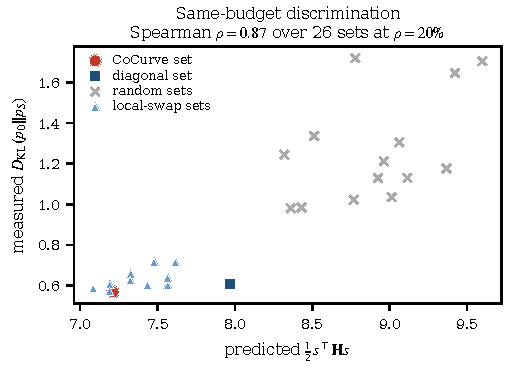
\includegraphics[width=0.62\columnwidth]{figures/fig_same_budget.pdf}
\caption{\textbf{The surrogate discriminates at one fixed budget.} Predicted
$\tfrac12 s^\top\Hmat s$ against measured $\KL(p_0\|p_S)$ over $26$ prunings matched to within
$0.75\%$ of the same removed cost on Llama-3.1-8B-Instruct at $\rho{=}20\%$: the \method and diagonal greedy sets, ten local swaps
of the former, and fourteen random sets. Every random set is above every structured one; within the
structured cluster the rank correlation is $0.55$.}
\label{fig:sameratio}
\end{figure}

\subsubsection{Sensitivity to the Surrogate Budget}
\label{app:sensitivity}
The edge estimator has two finite-budget knobs: the calibration size (number of sampled positions) and
the top-$r$ logit support of the Fisher-Gram features. Neither choice drives the result. We rebuild $\Hmat$ on the cheapest model (Llama-3.2-3B) at
top-$r\in\{128,256,512\}$ and calibration size $\in\{64,128\}$, then run each build through the
shipped selector -- the guard of \cref{app:protocol} and $\lambda$ re-chosen on held-out KL for that
build -- and evaluate (\cref{tab:sensitivity}). Across the builds measured, WikiText-2 perplexity spans
$3.1\%$ and MMLU $0.4$ points, while the $\hat\lambda$ each build selects moves by $20\%$. Doubling
top-$r$ from $256$ to $512$ is the sharpest case: it shifts $\hat\lambda$ from $0.0911$ to $0.0909$, a
different breakpoint of a different path, and returns the \emph{bit-identical} pruning --- the same
$133$ units, the same realised ratio, the same scores. The selection is therefore not sensitive to the
surrogate budget within the regime we use, and the insensitivity is not because nothing upstream
changed.
\Cref{fig:calibbudget} asks the same question of the selection directly rather than through a
benchmark: how many calibration sequences are needed before the chosen units stop changing.
\begin{table}[htbp]
\centering\caption{\textbf{Surrogate-budget sensitivity} (Llama-3.2-3B at $\rho{=}20\%$, under the
deployed guard). Upper block varies top-$r$ at fixed calibration $128$; lower block varies calibration
at fixed top-$256$. The default is $(128,256)$. Each build re-derives its own $\hat\lambda$, so the
column shows that the knob does move what the rule selects --- and the pruned model does not follow.}
\label{tab:sensitivity}\footnotesize
% generated by scripts/make_sensitivity_table.py -- do not edit by hand
\setlength{\tabcolsep}{7pt}
\begin{tabular}{ll ccc}
\toprule
knob & value & $\hat\lambda$ & Wiki\dn & MMLU\up\\
\midrule
top-$r$ & $128$ & $0.1094$ & 17.17 & .340\\
top-$r$ & $256$ (default) & $0.0911$ & 16.66 & .339\\
top-$r$ & $512$ & $0.0909$ & 16.66 & .339\\
\midrule
calib & $64$ & $0.1050$ & 16.82 & .336\\
calib & $128$ (default) & $0.0911$ & 16.66 & .339\\
\bottomrule
\end{tabular}

\end{table}

\begin{figure}[htbp]
\centering
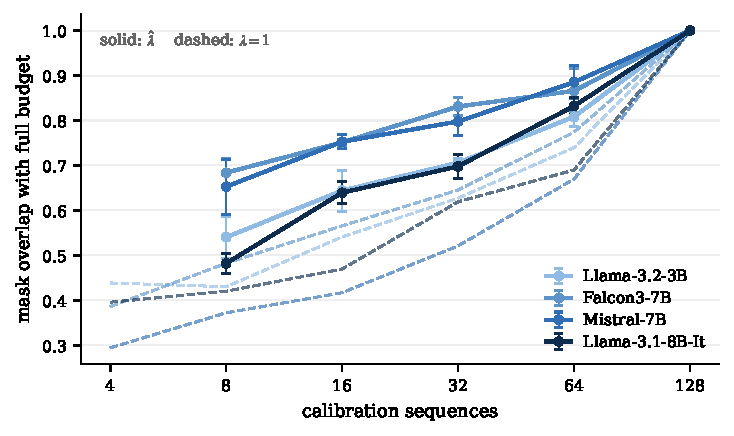
\includegraphics[width=0.62\textwidth]{figures/fig_calib_budget.pdf}
\caption{\textbf{How much calibration data the selection needs.} Overlap between the units chosen
from $n$ sequences and those chosen from the full budget of $128$, mean over three draws. Measuring
the selection rather than downstream accuracy separates estimator convergence from benchmark
resolution. At the calibrated $\hat\lambda$ the overlap is consistently higher than at
$\lambda{=}1$: damping the off-diagonal, the part of the matrix that needs the most data, also makes
the solution easier to estimate.}
\label{fig:calibbudget}
\end{figure}


\textbf{Calibration source.} C4 is our default, following the SparseGPT/Wanda convention, and the
comparison that justifies it rebuilds $\Hmat$ for Llama-3.1-8B-Instruct entirely from $128$
WikiText-2 sequences and re-runs the same $20\%$ selection. The two agree on which units matter and
differ exactly as source--target alignment predicts. Calibrating on WikiText buys a little WikiText
perplexity ($12.58$ against $12.91$) and a little on the other two corpora ($-1.0$ on PTB, $-0.7$ on
C4), and it costs accuracy on every capability task the two runs score identically: $-0.9$ on
ARC-challenge, $-1.3$ on ARC-easy, $-2.6$ on OpenBookQA, $-0.7$ on PIQA and $-3.8$ on WinoGrande.
The more diverse corpus is the better calibration source for everything except the corpus it is
matched against, which is why C4 is the default.

\textbf{Calibration draw.} Sensitivity to the draw itself is tested in two ways. Rebuilding $\Hmat$
from three independent samples of $128$ C4 sequences and selecting at $\lambda{=}1$ --- so that the draw
is the only thing that varies and the selection cannot absorb it --- leaves the result stable: WikiText-2
$13.11{\pm}0.22$, MMLU $38.1{\pm}0.7$, commonsense average $60.0{\pm}0.9$ over seeds $1/7/123$. That
isolates the estimator rather than the shipped configuration. The stronger test, rebuilding the curvature
from disjoint text and re-running the entire protocol at the model's own $\hat\lambda$, is reported on
Llama-3.2-3B in \cref{app:seed-variance}.

\subsection{Mechanism Analysis}

\label{app:mechanism}
\textbf{Bridge units.} With $d_u=\Hmat_{uu}$ and $b_u=\sum_{v\ne u}|\Hmat_{uv}|$,
\emph{bridge} units (low $d_u$, high $b_u$) are retained by \method but removed by diagonal pruning.

\textbf{A concrete bridge unit.} To make the phenomenon tangible, we single out one unit from the real
estimated $\Hmat$ of Llama-3.1-8B-Instruct. A representative bridge is an \emph{FFN channel group at
layer~1}. Its node saliency $\Hmat_{uu}$ places it in the \emph{bottom $31\%$} of all units, so a
node-first scorer (magnitude, activation, or diagonal Taylor) would rank it as safely prunable. Yet its coupling $b_u=\sum_{v\ne u}|\Hmat_{uv}|$ is in the \emph{top decile}: its strongest co-pruning edges run
to \emph{attention} units at layer~0 (a cross-module coupling, $|\Hmat_{uv}|\!\approx\!5.2\times10^{-3}$,
comparable to its own saliency $7.4\times10^{-3}$) and to FFN groups at layers~1--3 (cross-layer). This is
exactly the configuration \method is built to catch: a unit whose removal is cheap in isolation but
costly alongside the early-attention and nearby-FFN units it is coupled to. Diagonal pruning deletes it
together with those partners; \method retains it.

\textbf{Controlled causal test: bridge connectivity, not saliency, drives the damage.}
The bridge diagnosis above is structural, read off $\Hmat$; we confirm it is causal with a
matched-pair intervention, run on every model we build $\Hmat$ for. On each, we force-prune the bridge
units (low $d_u$, high $b_u$) and, as a control, an equal-size set drawn from the same low-saliency
pool but with low connectivity, matched unit-for-unit on saliency $d_u$, unit type and per-unit cost.
The remainder of the budget is one cost-normalised greedy fill, computed once and shared by both arms.
The two masks that result hold the same number of units, the same attention/FFN split, the same
removed cost and the same realised ratio to the last bit, and differ only in which low-saliency
population was forced out, so any gap isolates connectivity with saliency, type, cost and ratio all
held fixed. On Llama-3.1-8B-Instruct that is $169$ units each, $1.399\times10^{9}$ parameters,
realised ratio $0.2005$, $82$ units shared and $87$ forced.

Removing the high-connectivity units is far more destructive on capability
(\cref{tab:bridge-models}). Nineteen of the twenty capability cells fall, by up to $23.7$ points, even
though a node-first scorer rates the two forced sets equally prunable. Perplexity is not a reliable
witness to it. On three of the five models perplexity moves the \emph{other} way --- WikiText improves
by $4.5$, $5.5$ and $9.7$ while every capability group in those rows falls --- so on those the arm a
next-token proxy prefers is the arm that has lost the most capability. On Falcon3-7B the two arms are
within $0.8$ perplexity of each other, and on Mistral-Small-24B, where the intervention is by far the
most damaging, perplexity registers it in full ($+425.5$). The proxy is therefore free to point either
way at a fixed capability cost, which is the property that makes it unsafe to select on. That is the failure mode a node-first criterion
is built to walk into, and the one \method avoids by scoring the edges.

\textbf{How much of the selection the edge term moves.} Comparing the calibrated solution against
the pure diagonal one at $\rho{=}20\%$, the edge term moves between $1\%$ and $36\%$ of the removed
set across the five models, and the low end is the instructive case. On Mistral-Nemo-12B,
$\hat\lambda\!\approx\!2.4\times10^{-4}$ yields a set differing in three units out of $187$: an
attention head and an FFN group in layer $19$ that the diagonal selector removes and the edge term
holds back, and one FFN group in layer $24$ taken in their place, at an almost unchanged module split
(attention takes $16.2\%$ of the removed cost against $16.5\%$). Those three substitutions are worth
$3.1$ paired standard errors of held-out risk: the edge term corrects specific, identifiable units
rather than rewriting the selection.

\textbf{Where the effect is smallest.} Falcon3-7B is the one model on which a capability group does
not fall (Reading, $+0.8$), and it is also the model whose off-diagonal is least depth-graded of the
ten in \cref{tab:depth-grading} ($\rho_s(\ell_u,b_u)=-0.54$ against a median of $-0.87$) and the one
whose bridge corner is smallest ($30$ of $560$ units against $5$ to $14\%$ elsewhere). Less positional
structure in the off-diagonal, less for the edge term to protect, a smaller effect when it is removed
by force: the two orderings agree, on the model where they are most exposed.

\begin{table}[htbp]
\centering\footnotesize
\caption{\textbf{The bridge test, on every model we build $\Hmat$ for} ($\rho{=}20\%$). Low-saliency
units split by off-diagonal connectivity, matched unit-for-unit on saliency, unit type and cost, with
one greedy fill shared by both arms. Each pair holds the same number of units at the same removed cost
and the same realised ratio. Nineteen of the twenty capability cells fall; on three of the five models
perplexity moves the other way, on one it is flat, and on Mistral-Small-24B it agrees with them. The
Mistral-Small-24B pair is pruned on the second server and enters from its export ($170$ units per arm,
realised ratio $0.2014$).}
\label{tab:bridge-models}
% generated by scripts/make_bridge_models_table.py -- do not edit by hand
\footnotesize\setlength{\tabcolsep}{4pt}\renewcommand{\arraystretch}{1.02}
\begin{tabular}{@{}ll cccc c@{}}
\toprule
Model & Forced set & Commonsense\up & Science\up & Reading\up & Knowledge\up & Wiki\dn \\
\midrule
Llama-3.2-3B & Control & 58.5 & 42.9 & 45.7 & 35.2 & 31.8 \\
\rowours & Bridge & 48.8 & 36.9 & 41.5 & 30.7 & 26.2 \\
 & $\Delta$ & $-9.7$ & $-6.0$ & $-4.2$ & $-4.5$ & $-5.5$ \\
\addlinespace[2pt]
Falcon3-7B & Control & 60.3 & 48.8 & 52.4 & 38.4 & 7.3 \\
\rowours & Bridge & 55.8 & 43.4 & 53.1 & 37.1 & 8.1 \\
 & $\Delta$ & $-4.5$ & $-5.4$ & $+0.8$ & $-1.3$ & $+0.8$ \\
\addlinespace[2pt]
Llama-3.1-8B-It & Control & 66.5 & 53.0 & 52.2 & 40.5 & 22.8 \\
\rowours & Bridge & 53.6 & 38.9 & 45.6 & 32.0 & 18.3 \\
 & $\Delta$ & $-12.9$ & $-14.1$ & $-6.6$ & $-8.5$ & $-4.5$ \\
\addlinespace[2pt]
Mistral-Nemo-12B & Control & 64.5 & 51.8 & 57.1 & 40.1 & 23.3 \\
\rowours & Bridge & 53.1 & 39.3 & 41.5 & 31.7 & 13.6 \\
 & $\Delta$ & $-11.4$ & $-12.5$ & $-15.6$ & $-8.4$ & $-9.7$ \\
\addlinespace[2pt]
Mistral-Small-24B & Control & 63.9 & 51.7 & 57.3 & 40.7 & 14.4 \\
\rowours & Bridge & 40.9 & 29.3 & 33.6 & 25.9 & 439.9 \\
 & $\Delta$ & $-23.0$ & $-22.4$ & $-23.7$ & $-14.8$ & $+425.5$ \\
\bottomrule
\end{tabular}

\end{table}

\textbf{Layer pattern.} \Cref{fig:allocation} gives the per-layer, per-type profile on four models.
On Llama-3.1-8B-Instruct at $\rho{=}20\%$ the solution removes $46$ attention units and $105$ FFN
groups over $26$ of $32$ layers, at most nine in any one layer, and splits evenly over the second
half of the depth alone, $46$ attention against $46$ FFN.

\subsubsection{Fidelity to the Dense Model}
\label{app:fidelity}
The selection criterion is token-level KL to the dense model, so the first thing to check is
whether the pruned model actually reproduces the dense model's decisions more faithfully than the
alternatives do, and the second is what that fidelity buys. On
Llama-3.1-8B-Instruct at $\rho{=}30\%$ we measure, per task, the fraction of items on which each
pruned model predicts what dense predicts. \method is first or second on all six tasks examined and
first on three; LLM-Pruner takes the other three, by $0.1$ to $0.4$ points. Every other baseline is
behind both on every task. The objective does what it claims.

Splitting those items by whether \emph{dense} was right sharpens it: on PIQA, \method reproduces the
dense model on $81.8\%$ of the items dense answers correctly, the best of the eight methods. The
selection delivers the fidelity its objective asks for, and it does so without the benchmark ever
being consulted.
\subsection{Few-Shot Prompting}
\label{app:fewshot}
Zero-shot accuracy asks the model one question at a time. Five-shot prompting puts a long
demonstration prefix in front of the same question, which is where a pruned model has to carry more
context to answer the same item, the regime in which damage to attention would show first.
SlimGPT and 2SSP both report a few-shot number for that reason.

\Cref{tab:fewshot} gives MMLU at five shots, with demonstrations drawn from the dev split of the
subject being asked about and identical for every method. The ordering is the one the zero-shot
tables show: \method leads on both models at both reported ratios, by $0.6$ to $2.1$ points over the
strongest baseline. The advantage the selection buys is therefore not an artefact of the zero-shot
prompt format.

\begin{table}[htbp]
\centering
\caption{\textbf{MMLU at five shots} (\%). Demonstrations come from the dev split of each subject
and are identical for every method; dense accuracy in grey.}
\label{tab:fewshot}
% generated by scripts/make_fewshot_table.py -- do not edit by hand
\footnotesize\setlength{\tabcolsep}{6pt}\renewcommand{\arraystretch}{1.0}
\begin{tabular}{@{}ll rr r@{}}
\toprule
Model & $\rho$ & LLM-Pruner & SlimLLM & \method \\
\midrule
Llama-3.1-8B-Instruct \textcolor{gray}{(dense 50.8)} & 20\% & 34.9 & 34.8 & \textbf{37.0} \\
 & 30\% & 31.3 & 27.0 & \textbf{32.7} \\
\addlinespace[2pt]
Llama-3.2-3B \textcolor{gray}{(dense 41.5)} & 20\% & 33.0 & 31.0 & \textbf{33.6} \\
 & 30\% & 29.3 & 28.4 & \textbf{30.1} \\
\bottomrule
\end{tabular}

\end{table}

\subsection{Composition with Quantisation}
\label{app:quant}
Pruning and quantisation attack different redundancies: one removes units, the other lowers the
precision of what remains. Whether they compose is a deployment question, and it is not settled by
either measurement alone. If the two drew on the same slack, stacking them would cost more than
their separate costs suggest.

\Cref{tab:quant} pairs each model state with itself at bf16 and at $4$ bits, so the cost of
quantisation is a within-row difference and the dense row is the reference for what that cost should
be. On the dense model $4$ bits costs $5.7\%$ of perplexity and $0.8$ multiple-choice points. After
pruning to $\rho{=}30\%$ it costs $7.0\%$ and $1.8$ points, and at $\rho{=}40\%$ $13.1\%$ and $1.3$
points. The accuracy cost is therefore roughly what the dense model pays at both ratios, while the
perplexity cost grows as the remaining slack is spent, which is what a redundancy account
predicts, and small enough that the two compressions can be applied together.

The comparison arms turn this from a property of the pipeline into a property of the selection. The
two strongest baselines are quantised from their own pruned models under the identical quantiser and
load order, and the ordering after $4$ bits is the ordering before: \method reaches $23.1$ perplexity
and $49.9$ accuracy, against $29.2$ and $48.8$ for LLM-Pruner and $80.0$ and $44.9$ for SlimLLM.

Quantisation is close to additive with the selection, so a later decision to quantise does not make
the choice of which units to remove for the practitioner.

\begin{table}[htbp]
\centering
\caption{\textbf{Pruning composes with $4$-bit quantisation} (Llama-3.1-8B-Instruct). Each row is
one model state measured twice; the last two columns are the within-row cost of quantising it.
Perplexity on WikiText-2, accuracy the eight-task multiple-choice mean. The quantiser and the load
order are identical in every row.}
\label{tab:quant}
% generated by scripts/make_quant_table.py -- do not edit by hand
\footnotesize\setlength{\tabcolsep}{6pt}\renewcommand{\arraystretch}{1.02}
\begin{tabular}{@{}l rr rr rr@{}}
\toprule
& \multicolumn{2}{c}{bf16} & \multicolumn{2}{c}{$4$-bit} & \multicolumn{2}{c}{cost of $4$ bits}\\
\cmidrule(lr){2-3}\cmidrule(lr){4-5}\cmidrule(l){6-7}
Model state & Wiki\dn & MC\up & Wiki\dn & MC\up & Wiki\,\% & MC\,pt\\
\midrule
Dense & 6.4 & 67.2 & 6.8 & 66.4 & $+5.7$ & $-0.8$ \\
\addlinespace[2pt]
$\rho{=}30\%$ & & & & & & \\
\rowours \quad \method & 21.6 & 51.7 & 23.1 & 49.9 & $+7.0$ & $-1.8$ \\
\quad LLM-Pruner & 26.6 & 49.7 & 29.2 & 48.8 & $+9.7$ & $-0.9$ \\
\quad SlimLLM & 78.2 & 45.3 & 80.0 & 44.9 & $+2.2$ & $-0.4$ \\
\addlinespace[2pt]
$\rho{=}40\%$ & & & & & & \\
\rowours \quad \method & 59.1 & 43.5 & 66.9 & 42.2 & $+13.1$ & $-1.3$ \\
\bottomrule
\end{tabular}

\end{table}

\subsection{Robustness of the Selection}

\label{app:robustness}

Three questions about stability, each answered by a different perturbation: resampling the held-out
set, changing the selection protocol, and rebuilding the curvature from independent calibration text.
The third costs a full re-estimation, which we paid.

\subsection{How stable is the selected \texorpdfstring{$\lambda$}{lambda}?}
\label{app:lambda-robust}

Every number in this paper comes from one calibration draw and one held-out set of $16$ sequences.
Two questions follow, and they are different: whether the \emph{selection step} would survive a
different draw of the held-out set, and whether the \emph{curvature it selects over} would survive a
different draw of the calibration text. We answer both.

\paragraph{Resampling the held-out set collapses the candidate space.} The path files record the
per-sequence risk at every path point, so the bootstrap is exact and needs no further computation.
Over $26$ paths spanning ten models and five ratios, at $2000$ resamples each, the resampled
criterion reaches a median of $3.3\%$ of the members of the enumerated family, and $2.5\%$ at the
three ratios this paper reports. A typical family holds $318$ prunings and the whole bootstrap moves
among ten of them. The $5$--$95$ percentile of $\hat\lambda$ spans a median of $0.016$ of $[0,1]$,
and is under $0.05$ on $16$ of the $26$ paths.

What the criterion delivers is a pruning at the minimum rather than a distinguished value of
$\lambda$: evaluated back on the full held-out set, the mask a resample chooses costs a median of
$0.00\%$ additional risk over the one $\hat\lambda$ chooses, and every path puts at least $98.5\%$ of
resamples within one standard error of the minimum. The solution is piecewise constant and the path
is flat near its optimum, so the members the bootstrap moves among are the ones that cannot be told
apart.

\paragraph{Does the selected point hold up downstream?} The bootstrap judges $\hat\lambda$ by
held-out risk, the quantity it is selected on. The independent check is to take the selected point
and its neighbours and evaluate all of them on the full suite. On Llama-3.2-3B at $\rho{=}20\%$ we do
this for five points: $\hat\lambda$ itself, the two members at the edges of its $1$-SE band, and the
two nearest solutions just outside it. The selected point is within $0.3$ points of the best of the
five on three of the four capability groups and within $0.91$ on the fourth, and it is $2.7$ to $2.9$
points above the worst on the twelve-task mean. The criterion lands at the favourable end of the
region it cannot resolve.

\paragraph{Changing the protocol.} A bootstrap only perturbs the sample. We also varied the protocol
itself on Llama-3.1-8B-Instruct at $\rho{=}20\%$, one change at a time: the selection statistic
(KL $\rightarrow$ NLL), the number of held-out sequences ($16 \rightarrow 48$, pooling three
independent draws), and the draw itself (two further seeds). \emph{Four of these five variants select
the bit-identical solution}, $\hat\lambda = 0.0108$. The exception is changing the held-out domain
from C4 to WikiText, which moves $\hat\lambda$ to $0.0213$: a different breakpoint, the same order of
magnitude, and the direction one would predict when the evaluation corpus changes.

\paragraph{Holding the curvature fixed.} Both perturbations above act on the selection while $\Hmat$
stays as estimated. Perturbing the curvature itself, by rebuilding it from disjoint calibration text,
is a separate and more expensive question, and \cref{app:seed-variance} reports it.


\subsection{Rebuilding the curvature from independent calibration text}
\label{app:seed-variance}

\Cref{app:lambda-robust} perturbs the held-out set and the selection protocol but holds $\Hmat$
fixed. The question it cannot reach is whether a curvature estimate built from \emph{different text}
would lead anywhere else. Answering it means paying the full estimation cost a second time, which we
did. On Llama-3.2-3B we rebuilt $\Hmat$ from scratch (activation collection, all $672$ single-unit
ablations, Gram assembly) from a disjoint draw of the same sources, with its own held-out file, and
re-ran the identical protocol with no parameter changed.

\textbf{What the selector consumes transfers.} Diagonal saliency $d_u$ correlates at $0.99$ between
the two draws, and total coupling $b_u$, the quantity the bridge-unit argument rests on, at $0.96$.
This is the level at which the method reads $\Hmat$: the marginal of \cref{eq:marginal} contracts the
matrix against the selected set, and \cref{app:diagnostics} shows the same contraction is what the
split-half reproduction measures. Individual entries transfer less well than their aggregates, and the
selector consumes the aggregates.

\textbf{The selection moves, and the model does not.} $\hat\lambda$ goes from $0.0911$ to $0.0383$ and
the two prunings share $57.9\%$ of their removed units. At $\rho{=}20\%$ no capability group moves by
more than $0.81$ points (commonsense $-0.30$, science QA $+0.16$, reading $+0.42$, world knowledge
$+0.81$) and the twelve-task mean moves $+0.15$. Perplexity is within $2.1\%$ on two of three corpora
($-0.3\%$ WikiText, $-2.1\%$ C4) and $+14.0\%$ on PTB, the least stable of the three here as
elsewhere.

The three levels together say more than agreement would have. What the selector reads off $\Hmat$
transfers ($d_u$ at $0.99$, $b_u$ at $0.96$); the tie-breaking among units the marginal cannot
separate does not, and does not need to. The held-out
bootstrap shows the same structure from the other direction: mask agreement of $58.7\%$ alongside a
median excess risk of $0.00\%$. What transfers is the aggregate, which is what the method is asked to
deliver.


\subsection{Vision--Language Models: Per-Benchmark Results}
\label{app:vlm}

\textbf{Units and masking.} Units are attention heads --- grouped by shared key/value head where the
tower uses grouped-query attention --- and FFN channel groups, sixteen groups per layer, in
\emph{both} towers. A unit is removed by zeroing its slice of the input to the projection that writes
into the residual stream, exactly as in the text-only pipeline. The layer index is composite, so the
per-layer cap $\kappa{=}1.5\rho$ and the first/last-two-layer protection apply within each tower
rather than to a pooled index. Nothing else is added: no per-tower budget, no tower-level weighting,
and no new hyperparameter.

\textbf{Calibration.} $128$ image--caption pairs from Flickr30k \citep{young2014flickr30k} --- $192$ for Qwen2-VL-2B and $96$
for LLaVA-NeXT-7B, whose matrices were estimated under earlier budgets and left as they were. The
difference is a build-time budget on our own estimator and nothing else: every baseline draws its own
fixed calibration on every model alike ($64$ pairs for Wanda-sp and FLAP, $32$ for LLM-Pruner's
gradient pass), and the $48$ held-out pairs used to choose $\lambda$ are taken from the same
deterministic stream immediately \emph{after} that model's own calibration draw --- pairs
$128$--$175$ where the matrix saw $128$ or fewer, pairs $192$--$239$ on Qwen2-VL-2B --- so on every
model they are images the estimator never saw. Neither departure moves a comparison: a draw below
$128$ makes the off-diagonal noisier and the held-out criterion correspondingly more reluctant to
trust it, which costs our arm and no other; and the one model built on more carries the median of
our five headline margins, not the largest. The held-out pairs are used only for the $\lambda$ argmin and
enter nothing else. Flickr rather than COCO
is deliberate: SEED-Bench and several neighbouring suites are built on COCO images, so a COCO
calibration draw could place an evaluation image in the estimator. Scored positions are the caption
tokens only --- the prompt and the image placeholders are context, and scoring them would let a unit
look important for reproducing text the model was handed. The teacher support is
$\mathrm{top}\text{-}r{=}64$ rather than the $256$ used in the text-only experiments, because an
image-grounded sequence is expensive; splitting the scored positions into disjoint halves gives two
independent estimates of $\Hmat$ that correlate at $r{=}0.99$ on the off-diagonal, so the reduction
costs nothing that matters here.

\textbf{Evaluation.} Answers are scored by comparing the logits of the admissible answer tokens ---
option letters where the benchmark is multiple choice, the words \emph{yes} and \emph{no} where it is
binary --- at $1000$ items per benchmark. The dense model is measured under this same harness rather
than quoted, so every row is commensurable with every other. Retention is floor-corrected,
$(\text{arm}-c)/(\text{dense}-c)$, against the chance level $c$ of a selector that has learned
nothing: $25$ on the four-way multiple-choice suites (MMBench, SEED-Bench, ScienceQA, AI2D, MMStar)
and $50$ on the two binary ones (POPE, MME), giving $c{=}32.1$ for the seven-benchmark mean. Without
the correction a model at chance would read as a third of dense retained rather than zero.

\textbf{Baselines.} All are training-free and structured, and all receive the identical budget, guard,
calibration draw and scoring code. Magnitude scores a unit by the norm of \emph{all} the weights it
owns. Wanda-sp and FLAP are computed on the input channels of the output projection, where both are
defined; FLAP additionally standardises each layer's metric distribution to the global mean and
standard deviation before the global search, which is the half of that method that decides depth
allocation. LLM-Pruner is the first-order Taylor score $\sum |w \odot \partial \mathcal{L}/\partial
w|$ accumulated one image--caption pair per backward pass. The layer-drop arm is ShortGPT's
block-influence signal measured on the same calibration pass.

\textbf{The block-diagonal control.} One row of \cref{tab:vlm-full} is an arm rather than a
baseline. It re-runs our own selector on $\Hmat$ with the vision--language blocks set to zero,
holding the diagonal, the within-tower off-diagonal, the budget, the guard and the $\lambda$
protocol fixed --- the assumption a per-tower pruner makes without stating it, made explicit. On $8$
of the $21$ cells the two selectors return the same mask, so within-tower coupling alone already
fills the budget there; on the rest the masks differ and the seven-benchmark mean moves by $-1.2$ to
$+3.6$ points, its two largest values on LLaVA-1.5-7B. The cross-tower block is reported because it
is measurable, not because the shared budget depends on it: what \cref{sec:exp-vlm} asks of the
off-diagonal as a whole is the $\lambda{=}0$ comparison.

\textbf{Higher budgets.} At $\rho{=}40\%$ no selector in this comparison, ours included, retains a
third of its dense score above chance on any model, so that budget appears in \cref{tab:vlm-full}
and nowhere else: the numbers are measured, they are simply not a comparison. \Cref{app:vlm-recovery} reports what one
identical LoRA stage does to every arm at that budget.

{\scriptsize
\begin{center}
\captionof{table}{Vision--language models, per benchmark: the complete grid, the configurations the
body does not table included. Seven models at three ratios, ten arms each, every arm at $1000$ items
per benchmark; the block header repeats the ratio and the item count.
\textbf{Bold} is the best selector in the column, with the \method ablation excluded from that
comparison. \emph{cap.\ PPL} is perplexity on the held-out captions, the quantity the selection was
made against.}
\label{tab:vlm-full}
\end{center}
\begin{longtable}{@{}llrrrrrrrrrr@{}}
\toprule
Model & Selector & MMB & SEED & SQA & AI2D & MMStar & POPE & MME & Mean & \multicolumn{1}{c}{cap.\ PPL} & Ret. \\
\midrule
\endfirsthead
\toprule
Model & Selector & MMB & SEED & SQA & AI2D & MMStar & POPE & MME & Mean & \multicolumn{1}{c}{cap.\ PPL} & Ret. \\
\midrule
\endhead
\midrule
\multicolumn{12}{@{}l}{\textit{Qwen2-VL-2B, $\rho{=}20\%$, $1000$ items}} \\
& Dense & 78.6 & 62.4 & 80.5 & 73.0 & 44.6 & 88.4 & 83.6 & 73.0 & 15.39 &  \\
& \textbf{\method} & \textbf{65.1} & \textbf{51.9} & \textbf{57.1} & \textbf{50.3} & \textbf{38.2} & 85.9 & 66.5 & 59.3 & 17.37 & 66\% \\
& \quad block-diagonal $\Hmat$ & 65.9 & 51.9 & 53.0 & 46.9 & 36.0 & 81.8 & 74.8 & 58.6 & 18.18 & 65\% \\
& \quad diagonal only ($\lambda{=}0$) & 59.5 & 50.1 & 47.2 & 38.2 & 34.2 & 82.9 & 63.6 & 53.7 & 14.99 & 53\% \\
& LLM-Pruner & 57.6 & 50.2 & 51.5 & 48.5 & 32.3 & \textbf{87.2} & \textbf{71.7} & 57.0 & 18.01 & 61\% \\
& Wanda-sp & 59.0 & 49.6 & 55.3 & 39.0 & 31.4 & 74.6 & 51.6 & 51.5 & 18.33 & 47\% \\
& FLAP & 34.3 & 28.8 & 36.3 & 26.3 & 26.6 & 53.3 & 50.3 & 36.6 & 58.11 & 11\% \\
& ShortGPT (layer drop) & 30.6 & 27.5 & 32.7 & 22.3 & 24.9 & 61.0 & 49.5 & 35.5 & 17.10 & 8\% \\
& Magnitude & 43.1 & 32.8 & 41.8 & 28.3 & 25.9 & 58.5 & 51.5 & 40.3 & 25.05 & 20\% \\
& Random & 56.3 & 43.9 & 41.1 & 33.8 & 31.1 & 70.3 & 59.7 & 48.0 & 18.64 & 39\% \\
\midrule
\multicolumn{12}{@{}l}{\textit{Qwen2-VL-2B, $\rho{=}30\%$, $1000$ items}} \\
& Dense & 78.6 & 62.4 & 80.5 & 73.0 & 44.6 & 88.4 & 83.6 & 73.0 & 15.39 &  \\
& \textbf{\method} & 35.4 & 30.7 & 36.9 & 24.0 & 26.3 & 70.9 & 53.7 & 39.7 & 23.75 & 18\% \\
& \quad block-diagonal $\Hmat$ & 36.0 & 32.6 & 36.5 & 24.0 & 26.6 & 66.0 & 54.4 & 39.4 & 23.39 & 18\% \\
& \quad diagonal only ($\lambda{=}0$) & 34.4 & 31.1 & 35.9 & 24.6 & 27.1 & 62.1 & 49.7 & 37.8 & 25.84 & 14\% \\
& LLM-Pruner & \textbf{42.3} & \textbf{37.6} & \textbf{41.1} & \textbf{28.5} & 26.6 & \textbf{76.4} & \textbf{61.6} & 44.9 & 25.70 & 31\% \\
& Wanda-sp & 34.3 & 29.6 & 36.3 & 23.9 & 26.8 & 71.1 & 59.9 & 40.3 & 27.64 & 20\% \\
& FLAP & 33.4 & 29.3 & 36.5 & 23.9 & \textbf{27.4} & 51.2 & 50.8 & 36.1 & 138.28 & 10\% \\
& ShortGPT (layer drop) & 33.8 & 29.6 & 36.0 & 24.3 & 27.3 & 49.6 & 50.7 & 35.9 & 26.40 & 9\% \\
& Magnitude & 33.9 & 30.3 & 34.4 & 25.9 & 25.4 & 58.4 & 49.0 & 36.8 & 77.09 & 11\% \\
& Random & 34.2 & 29.2 & 36.4 & 27.2 & 26.9 & 50.8 & 49.3 & 36.3 & 129.57 & 10\% \\
\midrule
\multicolumn{12}{@{}l}{\textit{Qwen2-VL-2B, $\rho{=}40\%$, $1000$ items}} \\
& Dense & 78.6 & 62.4 & 80.5 & 73.0 & 44.6 & 88.4 & 83.6 & 73.0 & 15.39 &  \\
& \textbf{\method} & 34.2 & \textbf{30.1} & 35.3 & 23.9 & 27.5 & \textbf{53.2} & \textbf{50.7} & 36.4 & 61.60 & 10\% \\
& \quad block-diagonal $\Hmat$ & 34.4 & 29.2 & 35.4 & 23.6 & 27.2 & 52.2 & 53.6 & 36.5 & 61.06 & 11\% \\
& \quad diagonal only ($\lambda{=}0$) & 34.4 & 29.8 & 35.5 & 23.6 & 27.2 & 54.5 & 49.9 & 36.4 & 73.93 & 10\% \\
& LLM-Pruner & \textbf{34.3} & 29.8 & 35.4 & 23.2 & 27.3 & 51.1 & 50.3 & 35.9 & 50.78 & 9\% \\
& Wanda-sp & 33.9 & 29.5 & 34.9 & 23.6 & 27.3 & 51.0 & 49.2 & 35.6 & 122.79 & 9\% \\
& FLAP & 31.8 & 27.4 & \textbf{37.2} & 24.6 & 28.4 & 51.2 & 49.4 & 35.7 & 301.08 & 9\% \\
& ShortGPT (layer drop) & 32.7 & 28.7 & 34.1 & \textbf{24.7} & 28.8 & 52.7 & 48.3 & 35.7 & 165.43 & 9\% \\
& Magnitude & 29.7 & 24.0 & 34.8 & 24.0 & \textbf{29.4} & 51.0 & 49.2 & 34.6 & 235.66 & 6\% \\
& Random & 29.3 & 24.7 & 36.0 & 23.8 & 27.3 & 48.5 & 49.2 & 34.1 & 957.02 & 5\% \\
\midrule
\multicolumn{12}{@{}l}{\textit{Qwen2.5-VL-3B, $\rho{=}20\%$, $1000$ items}} \\
& Dense & 83.8 & 65.2 & 80.9 & 80.9 & 56.4 & 89.8 & 85.0 & 77.4 & 13.15 &  \\
& \textbf{\method} & \textbf{70.5} & 56.0 & 60.5 & \textbf{58.9} & 42.2 & \textbf{89.7} & \textbf{71.0} & 64.1 & 15.64 & 71\% \\
& \quad block-diagonal $\Hmat$ & 69.6 & 56.2 & 68.0 & 57.6 & 44.0 & 89.3 & 71.5 & 65.2 & 15.05 & 73\% \\
& \quad diagonal only ($\lambda{=}0$) & 70.0 & 58.4 & 65.6 & 60.2 & 42.6 & 81.3 & 72.7 & 64.4 & 16.09 & 71\% \\
& LLM-Pruner & 70.4 & \textbf{57.6} & \textbf{61.6} & \textbf{58.9} & \textbf{43.7} & 87.8 & 70.5 & 64.4 & 15.38 & 71\% \\
& Wanda-sp & 65.2 & 52.5 & 59.1 & 54.4 & 38.0 & 70.9 & 65.8 & 58.0 & 18.01 & 57\% \\
& FLAP & 32.5 & 27.7 & 33.4 & 26.9 & 30.9 & 62.3 & 52.3 & 38.0 & 95.87 & 13\% \\
& ShortGPT (layer drop) & 56.4 & 38.9 & 49.5 & 34.5 & 32.2 & 88.2 & 68.8 & 52.6 & 15.86 & 45\% \\
& Magnitude & 29.7 & 28.1 & 35.3 & 25.7 & 25.7 & 49.3 & 51.7 & 35.1 & 3396.11 & 6\% \\
& Random & 62.4 & 48.8 & 55.8 & 42.0 & 40.5 & 74.4 & 55.2 & 54.2 & 20.24 & 49\% \\
\midrule
\multicolumn{12}{@{}l}{\textit{Qwen2.5-VL-3B, $\rho{=}30\%$, $1000$ items}} \\
& Dense & 83.8 & 65.2 & 80.9 & 80.9 & 56.4 & 89.8 & 85.0 & 77.4 & 13.15 &  \\
& \textbf{\method} & \textbf{57.0} & \textbf{45.1} & 44.1 & \textbf{34.2} & \textbf{33.1} & 72.1 & 64.3 & 50.0 & 21.86 & 39\% \\
& \quad block-diagonal $\Hmat$ & 53.4 & 44.5 & 42.3 & 33.3 & 32.8 & 68.0 & 62.9 & 48.2 & 20.53 & 35\% \\
& \quad diagonal only ($\lambda{=}0$) & 44.5 & 35.6 & 40.2 & 30.2 & 26.5 & 67.8 & 55.7 & 42.9 & 19.90 & 24\% \\
& LLM-Pruner & 51.1 & 41.5 & \textbf{48.0} & 31.9 & 28.3 & \textbf{82.9} & \textbf{65.2} & 49.8 & 23.46 & 39\% \\
& Wanda-sp & 47.6 & 32.4 & 41.6 & 30.8 & 28.0 & 57.8 & 52.4 & 41.5 & 21.81 & 21\% \\
& FLAP & 30.9 & 28.0 & 36.8 & 26.5 & 28.1 & 50.5 & 50.4 & 35.9 & 261.11 & 8\% \\
& ShortGPT (layer drop) & 32.1 & 24.0 & 37.0 & 28.1 & 24.1 & 49.8 & 50.3 & 35.1 & 24.78 & 6\% \\
& Magnitude & 31.3 & 27.4 & 36.9 & 24.7 & 26.2 & 50.1 & 49.9 & 35.2 & 8909.21 & 7\% \\
& Random & 31.5 & 30.5 & 35.8 & 25.8 & 23.3 & 48.2 & 49.3 & 34.9 & 56.61 & 6\% \\
\midrule
\multicolumn{12}{@{}l}{\textit{Qwen2.5-VL-3B, $\rho{=}40\%$, $1000$ items}} \\
& Dense & 83.8 & 65.2 & 80.9 & 80.9 & 56.4 & 89.8 & 85.0 & 77.4 & 13.15 &  \\
& \textbf{\method} & \textbf{33.8} & 26.5 & 36.4 & 23.9 & 27.7 & 56.1 & 49.1 & 36.2 & 55.67 & 9\% \\
& \quad block-diagonal $\Hmat$ & 32.2 & 28.0 & 37.3 & 24.4 & 27.8 & 56.8 & 51.2 & 36.8 & 48.49 & 10\% \\
& \quad diagonal only ($\lambda{=}0$) & 34.2 & 29.7 & 38.9 & 25.5 & 27.1 & 57.4 & 55.4 & 38.3 & 59.95 & 14\% \\
& LLM-Pruner & 30.3 & 27.0 & 35.1 & 24.7 & 26.0 & \textbf{56.7} & \textbf{50.3} & 35.7 & 51.45 & 8\% \\
& Wanda-sp & 32.6 & 26.4 & 35.5 & \textbf{27.9} & 25.2 & 55.0 & 49.1 & 36.0 & 37.39 & 8\% \\
& FLAP & 31.0 & 25.6 & 34.9 & 24.9 & 23.6 & 53.7 & 50.1 & 34.8 & 1239.02 & 6\% \\
& ShortGPT (layer drop) & 31.1 & 27.3 & 33.9 & 27.2 & 25.0 & 51.5 & 50.1 & 35.2 & 31.37 & 7\% \\
& Magnitude & 32.1 & 26.8 & 36.7 & 25.8 & \textbf{28.8} & 49.0 & 48.7 & 35.4 & 18629.02 & 7\% \\
& Random & 32.4 & \textbf{27.4} & \textbf{38.0} & 25.7 & 26.6 & 50.7 & 49.4 & 35.7 & 404.45 & 8\% \\
\midrule
\multicolumn{12}{@{}l}{\textit{Qwen2.5-VL-7B, $\rho{=}20\%$, $1000$ items}} \\
& Dense & 86.7 & 70.5 & 88.5 & 84.5 & 63.8 & 89.6 & 87.3 & 81.6 & 20.53 &  \\
& \textbf{\method} & \textbf{81.9} & \textbf{67.1} & 77.8 & \textbf{75.2} & 51.5 & 86.9 & 80.5 & 74.4 & 17.96 & 86\% \\
& \quad block-diagonal $\Hmat$ & 81.4 & 67.1 & 78.2 & 74.2 & 51.6 & 86.6 & 80.2 & 74.2 & 18.00 & 85\% \\
& \quad diagonal only ($\lambda{=}0$) & 81.1 & 66.3 & 75.4 & 70.6 & 53.9 & 87.6 & 79.4 & 73.5 & 16.27 & 84\% \\
& LLM-Pruner & 80.5 & 61.9 & \textbf{78.8} & 73.6 & 52.5 & 84.7 & 73.5 & 72.2 & 19.22 & 81\% \\
& Wanda-sp & 73.8 & 56.7 & 72.0 & 63.5 & 43.2 & 74.4 & 56.5 & 62.9 & 17.43 & 62\% \\
& FLAP & 80.4 & 63.4 & 78.6 & 70.5 & 50.6 & \textbf{88.6} & 80.9 & 73.3 & 15.17 & 83\% \\
& ShortGPT (layer drop) & 31.5 & 28.9 & 35.6 & 24.3 & 26.6 & 51.0 & 49.0 & 35.3 & 433.69 & 6\% \\
& Magnitude & 79.9 & 65.1 & 73.1 & 69.9 & \textbf{53.6} & 87.3 & \textbf{81.7} & 72.9 & 14.51 & 83\% \\
& Random & 71.4 & 61.2 & 70.1 & 61.9 & 43.5 & 80.1 & 62.3 & 64.4 & 16.34 & 65\% \\
\midrule
\multicolumn{12}{@{}l}{\textit{Qwen2.5-VL-7B, $\rho{=}30\%$, $1000$ items}} \\
& Dense & 86.7 & 70.5 & 88.5 & 84.5 & 63.8 & 89.6 & 87.3 & 81.6 & 20.53 &  \\
& \textbf{\method} & \textbf{68.1} & \textbf{59.7} & 59.5 & \textbf{55.3} & \textbf{41.5} & \textbf{90.7} & 70.1 & 63.6 & 19.88 & 64\% \\
& \quad block-diagonal $\Hmat$ & 68.3 & 59.6 & 59.6 & 55.3 & 40.7 & 90.8 & 70.9 & 63.6 & 19.84 & 64\% \\
& \quad diagonal only ($\lambda{=}0$) & 67.7 & 55.8 & 55.5 & 52.6 & 40.6 & 84.9 & 70.5 & 61.1 & 17.48 & 59\% \\
& LLM-Pruner & 61.5 & 43.4 & \textbf{59.9} & 43.6 & 37.2 & 82.3 & \textbf{72.2} & 57.2 & 18.12 & 51\% \\
& Wanda-sp & 63.4 & 44.3 & 54.0 & 44.6 & 33.3 & 71.3 & 54.2 & 52.2 & 19.21 & 41\% \\
& FLAP & 65.6 & 50.5 & 58.2 & 45.1 & 35.7 & 83.2 & 71.5 & 58.5 & 15.91 & 53\% \\
& ShortGPT (layer drop) & 32.5 & 29.5 & 35.7 & 23.0 & 25.6 & 51.0 & 49.1 & 35.2 & 3811.02 & 6\% \\
& Magnitude & 65.2 & 54.9 & 56.0 & 39.5 & 38.4 & 84.4 & \textbf{72.2} & 58.7 & 17.94 & 54\% \\
& Random & 58.7 & 44.3 & 46.1 & 33.8 & 37.6 & 52.1 & 50.7 & 46.2 & 24.24 & 28\% \\
\midrule
\multicolumn{12}{@{}l}{\textit{Qwen2.5-VL-7B, $\rho{=}40\%$, $1000$ items}} \\
& Dense & 86.7 & 70.5 & 88.5 & 84.5 & 63.8 & 89.6 & 87.3 & 81.6 & 20.53 &  \\
& \textbf{\method} & \textbf{45.4} & \textbf{35.9} & \textbf{41.9} & 30.7 & 27.7 & 72.7 & 53.4 & 44.0 & 26.68 & 24\% \\
& \quad block-diagonal $\Hmat$ & 45.4 & 35.9 & 41.9 & 30.7 & 27.7 & 72.7 & 53.4 & 44.0 & 26.68 & 24\% \\
& \quad diagonal only ($\lambda{=}0$) & 50.5 & 39.2 & 43.7 & 34.1 & 31.7 & 69.9 & 59.5 & 46.9 & 29.32 & 30\% \\
& LLM-Pruner & 45.3 & 35.4 & 38.2 & \textbf{32.2} & \textbf{29.6} & 61.0 & \textbf{60.5} & 43.2 & 24.86 & 22\% \\
& Wanda-sp & 30.8 & 26.5 & 36.8 & 25.6 & 27.3 & 48.7 & 49.7 & 35.1 & 38.08 & 6\% \\
& FLAP & 38.4 & 30.3 & 36.2 & 26.0 & 25.2 & \textbf{75.3} & 59.9 & 41.6 & 25.25 & 19\% \\
& ShortGPT (layer drop) & 32.7 & 28.7 & 36.2 & 24.3 & 25.6 & 49.3 & 50.4 & 35.3 & 1131.56 & 6\% \\
& Magnitude & 38.7 & 34.1 & 39.2 & 29.2 & 27.8 & 66.5 & 56.1 & 41.7 & 27.43 & 19\% \\
& Random & 38.1 & 30.3 & 37.1 & 23.2 & 26.0 & 48.2 & 50.3 & 36.2 & 32.18 & 8\% \\
\midrule
\multicolumn{12}{@{}l}{\textit{Qwen3-VL-8B, $\rho{=}20\%$, $1000$ items}} \\
& Dense & 89.7 & 69.4 & 94.4 & 84.8 & 66.9 & 90.4 & 88.4 & 83.4 & 19.41 &  \\
& \textbf{\method} & \textbf{81.1} & 61.8 & \textbf{76.3} & \textbf{69.2} & \textbf{52.4} & \textbf{88.7} & 68.0 & 71.1 & 18.10 & 76\% \\
& \quad block-diagonal $\Hmat$ & 80.4 & 61.7 & 75.9 & 68.9 & 52.0 & 88.5 & 67.8 & 70.7 & 18.10 & 75\% \\
& \quad diagonal only ($\lambda{=}0$) & 72.8 & 59.1 & 68.4 & 59.7 & 45.4 & 88.7 & 71.6 & 66.5 & 13.43 & 67\% \\
& LLM-Pruner & 74.3 & \textbf{63.1} & 74.5 & 60.4 & 46.5 & 81.7 & 60.4 & 65.8 & 19.12 & 66\% \\
& Wanda-sp & 38.3 & 33.8 & 46.0 & 33.7 & 27.6 & 52.2 & 51.8 & 40.5 & 26.49 & 16\% \\
& FLAP & 74.9 & 61.4 & 69.8 & 62.4 & 47.6 & 88.5 & \textbf{74.5} & 68.4 & 15.54 & 71\% \\
& ShortGPT (layer drop) & 30.1 & 26.1 & 38.1 & 26.2 & 26.0 & 48.8 & 51.1 & 35.2 & 9093.50 & 6\% \\
& Magnitude & 68.4 & 57.3 & 62.6 & 57.9 & 43.3 & 58.0 & 51.2 & 57.0 & 15.82 & 48\% \\
& Random & 59.7 & 44.5 & 48.2 & 34.8 & 35.6 & 85.0 & 68.7 & 53.8 & 19.26 & 42\% \\
\midrule
\multicolumn{12}{@{}l}{\textit{Qwen3-VL-8B, $\rho{=}30\%$, $1000$ items}} \\
& Dense & 89.7 & 69.4 & 94.4 & 84.8 & 66.9 & 90.4 & 88.4 & 83.4 & 19.41 &  \\
& \textbf{\method} & \textbf{62.6} & \textbf{53.2} & \textbf{54.2} & \textbf{47.3} & \textbf{39.3} & 83.9 & \textbf{63.7} & 57.7 & 25.40 & 50\% \\
& \quad block-diagonal $\Hmat$ & 63.0 & 52.8 & 54.2 & 47.7 & 38.4 & 83.7 & 63.6 & 57.6 & 25.40 & 50\% \\
& \quad diagonal only ($\lambda{=}0$) & 49.2 & 43.7 & 46.5 & 33.1 & 33.7 & 83.3 & 61.2 & 50.1 & 25.43 & 35\% \\
& LLM-Pruner & 43.4 & 47.1 & 39.5 & 25.0 & 29.5 & \textbf{85.4} & 59.0 & 47.0 & 30.17 & 29\% \\
& Wanda-sp & 34.5 & 29.6 & 36.1 & 23.8 & 27.5 & 49.0 & 50.8 & 35.9 & 48.60 & 7\% \\
& FLAP & 42.2 & 41.3 & 42.4 & 28.8 & 31.4 & 82.5 & 57.0 & 46.5 & 24.95 & 28\% \\
& ShortGPT (layer drop) & 33.2 & 27.4 & 34.8 & 23.1 & 28.1 & 49.5 & 50.8 & 35.3 & 41895.50 & 6\% \\
& Magnitude & 34.9 & 29.8 & 35.0 & 24.5 & 27.5 & 59.6 & 52.4 & 37.7 & 55.45 & 11\% \\
& Random & 41.6 & 36.5 & 36.9 & 28.3 & 30.4 & 63.0 & 51.9 & 41.2 & 35.15 & 18\% \\
\midrule
\multicolumn{12}{@{}l}{\textit{Qwen3-VL-8B, $\rho{=}40\%$, $1000$ items}} \\
& Dense & 89.7 & 69.4 & 94.4 & 84.8 & 66.9 & 90.4 & 88.4 & 83.4 & 19.41 &  \\
& \textbf{\method} & 34.5 & 30.0 & 34.9 & 23.5 & \textbf{27.4} & 52.1 & \textbf{51.9} & 36.3 & 179.42 & 8\% \\
& \quad block-diagonal $\Hmat$ & 34.5 & 30.0 & 34.9 & 23.5 & 27.4 & 52.1 & 51.9 & 36.3 & 179.42 & 8\% \\
& \quad diagonal only ($\lambda{=}0$) & 34.7 & 29.5 & 34.9 & 23.5 & 27.1 & 50.4 & 52.7 & 36.1 & 238.44 & 8\% \\
& LLM-Pruner & \textbf{34.6} & 29.8 & 36.1 & 23.3 & 26.8 & 49.0 & \textbf{51.9} & 35.9 & 166.53 & 7\% \\
& Wanda-sp & 34.3 & 29.6 & 34.9 & 24.0 & \textbf{27.4} & 48.2 & 48.7 & 35.3 & 1035.76 & 6\% \\
& FLAP & 34.2 & 29.8 & 35.5 & 23.5 & 27.2 & \textbf{64.0} & 51.3 & 37.9 & 66.41 & 11\% \\
& ShortGPT (layer drop) & 29.9 & 26.2 & \textbf{36.5} & 22.7 & 24.8 & 49.3 & 50.4 & 34.3 & 147864.18 & 4\% \\
& Magnitude & 34.1 & \textbf{30.4} & 36.0 & 23.1 & 26.7 & 50.5 & 50.8 & 35.9 & 787.21 & 7\% \\
& Random & 33.9 & 29.7 & 35.9 & \textbf{25.1} & 27.2 & 52.3 & 50.9 & 36.4 & 98.81 & 8\% \\
\midrule
\multicolumn{12}{@{}l}{\textit{InternVL3-8B, $\rho{=}20\%$, $1000$ items}} \\
& Dense & 88.2 & 67.4 & 97.5 & 83.7 & 67.1 & 93.3 & 88.1 & 83.6 & 14.05 &  \\
& \textbf{\method} & \textbf{83.7} & \textbf{64.2} & 82.7 & 72.3 & \textbf{53.8} & \textbf{92.5} & \textbf{82.3} & 75.9 & 14.04 & 85\% \\
& \quad block-diagonal $\Hmat$ & 83.7 & 64.2 & 82.7 & 72.3 & 53.8 & 92.5 & 82.3 & 75.9 & 14.04 & 85\% \\
& \quad diagonal only ($\lambda{=}0$) & 81.0 & 62.0 & 77.9 & 71.0 & 53.3 & 91.0 & 80.8 & 73.9 & 15.04 & 81\% \\
& LLM-Pruner & 78.4 & 61.8 & 78.7 & 68.4 & 52.2 & 84.0 & 79.0 & 71.8 & 14.53 & 77\% \\
& Wanda-sp & 50.0 & 36.3 & 62.6 & 47.0 & 31.9 & 65.8 & 55.1 & 49.8 & 19.17 & 34\% \\
& FLAP & 80.7 & 62.1 & \textbf{84.8} & \textbf{73.8} & 52.6 & 88.3 & 81.2 & 74.8 & 14.72 & 83\% \\
& ShortGPT (layer drop) & 33.8 & 32.2 & 61.7 & 51.5 & 24.1 & 51.0 & 49.2 & 43.4 & 20.33 & 22\% \\
& Magnitude & 79.8 & 57.7 & 74.6 & 64.1 & 48.3 & 91.1 & 79.3 & 70.7 & 13.46 & 75\% \\
& Random & 72.9 & 61.0 & 74.3 & 62.9 & 49.7 & 87.0 & 67.6 & 67.9 & 14.68 & 69\% \\
\midrule
\multicolumn{12}{@{}l}{\textit{InternVL3-8B, $\rho{=}30\%$, $1000$ items}} \\
& Dense & 88.2 & 67.4 & 97.5 & 83.7 & 67.1 & 93.3 & 88.1 & 83.6 & 14.05 &  \\
& \textbf{\method} & 67.7 & 54.0 & 59.6 & 52.7 & 41.6 & \textbf{89.0} & \textbf{71.9} & 62.4 & 16.64 & 59\% \\
& \quad block-diagonal $\Hmat$ & 67.7 & 54.0 & 59.6 & 52.7 & 41.6 & 89.0 & 71.9 & 62.4 & 16.64 & 59\% \\
& \quad diagonal only ($\lambda{=}0$) & 62.2 & 49.1 & 54.0 & 50.3 & 36.0 & 80.0 & 56.9 & 55.5 & 17.30 & 45\% \\
& LLM-Pruner & 65.3 & 53.2 & 61.4 & 52.5 & 40.4 & 84.8 & 64.7 & 60.3 & 19.31 & 55\% \\
& Wanda-sp & 49.2 & 36.3 & 51.5 & 34.8 & 28.6 & 56.5 & 58.3 & 45.0 & 21.74 & 25\% \\
& FLAP & \textbf{74.5} & \textbf{56.1} & \textbf{65.0} & \textbf{54.7} & \textbf{42.1} & 83.6 & 53.1 & 61.3 & 18.27 & 57\% \\
& ShortGPT (layer drop) & 31.8 & 29.5 & 37.8 & 26.3 & 25.7 & 49.7 & 48.9 & 35.7 & 26.04 & 7\% \\
& Magnitude & 47.5 & 42.2 & 46.0 & 32.1 & 30.2 & 65.8 & 52.3 & 45.2 & 17.41 & 25\% \\
& Random & 58.9 & 45.0 & 48.7 & 38.6 & 34.9 & 62.5 & 57.9 & 49.5 & 19.48 & 34\% \\
\midrule
\multicolumn{12}{@{}l}{\textit{InternVL3-8B, $\rho{=}40\%$, $1000$ items}} \\
& Dense & 88.2 & 67.4 & 97.5 & 83.7 & 67.1 & 93.3 & 88.1 & 83.6 & 14.05 &  \\
& \textbf{\method} & \textbf{38.3} & \textbf{32.8} & 37.8 & \textbf{27.2} & \textbf{30.7} & 51.0 & 49.4 & 38.2 & 29.28 & 12\% \\
& \quad block-diagonal $\Hmat$ & 38.3 & 32.8 & 37.8 & 27.2 & 30.7 & 51.0 & 49.4 & 38.2 & 29.28 & 12\% \\
& \quad diagonal only ($\lambda{=}0$) & 36.8 & 27.7 & 37.5 & 24.6 & 26.7 & 51.0 & 49.0 & 36.2 & 31.03 & 8\% \\
& LLM-Pruner & 36.1 & 29.4 & \textbf{37.9} & 23.7 & 28.5 & \textbf{57.5} & 49.2 & 37.5 & 66.94 & 10\% \\
& Wanda-sp & 35.0 & 28.5 & 34.0 & 24.9 & 28.8 & 51.1 & 49.3 & 35.9 & 56.20 & 7\% \\
& FLAP & 34.6 & 31.8 & 35.3 & 25.1 & 29.2 & 51.5 & 48.0 & 36.5 & 101.33 & 8\% \\
& ShortGPT (layer drop) & 31.3 & 28.3 & 35.4 & 25.8 & 26.6 & 51.1 & 50.3 & 35.5 & 70.42 & 7\% \\
& Magnitude & 35.7 & 30.0 & 36.2 & 23.1 & 27.0 & 52.9 & 52.2 & 36.7 & 33.12 & 9\% \\
& Random & 37.6 & 30.0 & 37.8 & 26.5 & 29.7 & 55.6 & \textbf{52.6} & 38.5 & 47.66 & 12\% \\
\midrule
\multicolumn{12}{@{}l}{\textit{LLaVA-NeXT-7B, $\rho{=}20\%$, $1000$ items}} \\
& Dense & 76.5 & 64.5 & 73.5 & 68.0 & 38.3 & 90.2 & 79.0 & 70.0 & 16.70 &  \\
& \textbf{\method} & 70.5 & 57.0 & 61.7 & 54.7 & 36.8 & 90.8 & 70.9 & 63.2 & 15.96 & 82\% \\
& \quad block-diagonal $\Hmat$ & 70.5 & 57.0 & 61.7 & 54.7 & 36.8 & 90.8 & 70.9 & 63.2 & 15.96 & 82\% \\
& \quad diagonal only ($\lambda{=}0$) & 70.5 & 57.0 & 61.7 & 54.7 & 36.8 & 90.8 & 70.9 & 63.2 & 15.96 & 82\% \\
& LLM-Pruner & \textbf{71.8} & 60.0 & 61.2 & \textbf{55.3} & 36.8 & 85.5 & 73.5 & 63.4 & 17.46 & 83\% \\
& Wanda-sp & 41.5 & 36.1 & 37.2 & 27.8 & 25.4 & 57.6 & 55.2 & 40.1 & 23.13 & 21\% \\
& FLAP & 70.9 & \textbf{61.6} & 61.5 & 54.0 & \textbf{38.0} & 89.2 & 71.9 & 63.9 & 17.89 & 84\% \\
& ShortGPT (layer drop) & 34.3 & 29.8 & 35.5 & 23.6 & 27.1 & 51.0 & 49.2 & 35.8 & 38085.10 & 10\% \\
& Magnitude & 67.8 & 58.4 & \textbf{62.4} & 51.7 & 36.3 & \textbf{91.2} & 72.9 & 63.0 & 18.97 & 81\% \\
& Random & 66.5 & 53.5 & 59.6 & 48.7 & 32.8 & 88.9 & \textbf{74.4} & 60.6 & 18.49 & 75\% \\
\midrule
\multicolumn{12}{@{}l}{\textit{LLaVA-NeXT-7B, $\rho{=}30\%$, $1000$ items}} \\
& Dense & 76.5 & 64.5 & 73.5 & 68.0 & 38.3 & 90.2 & 79.0 & 70.0 & 16.70 &  \\
& \textbf{\method} & 56.3 & 45.5 & 44.5 & 36.1 & 33.0 & \textbf{89.6} & \textbf{66.2} & 53.0 & 18.71 & 55\% \\
& \quad block-diagonal $\Hmat$ & 56.3 & 45.5 & 44.5 & 36.1 & 33.0 & 89.6 & 66.2 & 53.0 & 18.71 & 55\% \\
& \quad diagonal only ($\lambda{=}0$) & 49.3 & 41.8 & 42.4 & 36.7 & 31.7 & 88.8 & 64.4 & 50.7 & 17.73 & 49\% \\
& LLM-Pruner & \textbf{65.7} & \textbf{56.1} & 53.6 & \textbf{47.1} & \textbf{34.0} & 88.5 & 56.9 & 57.4 & 21.59 & 67\% \\
& Wanda-sp & 36.3 & 29.7 & 35.5 & 25.1 & 25.9 & 49.0 & 50.6 & 36.0 & 24.74 & 10\% \\
& FLAP & 39.4 & 35.3 & 43.2 & 30.1 & 27.3 & 66.5 & 61.5 & 43.3 & 25.22 & 30\% \\
& ShortGPT (layer drop) & 36.4 & 30.3 & 35.9 & 28.2 & 25.6 & 59.6 & 54.6 & 38.7 & 27.54 & 17\% \\
& Magnitude & 57.1 & 46.8 & 45.7 & 35.7 & 32.1 & 88.2 & 62.9 & 52.6 & 26.41 & 54\% \\
& Random & 62.2 & 49.0 & \textbf{53.9} & 42.7 & 30.0 & 87.9 & 62.5 & 55.5 & 21.38 & 62\% \\
\midrule
\multicolumn{12}{@{}l}{\textit{LLaVA-NeXT-7B, $\rho{=}40\%$, $1000$ items}} \\
& Dense & 76.5 & 64.5 & 73.5 & 68.0 & 38.3 & 90.2 & 79.0 & 70.0 & 16.70 &  \\
& \textbf{\method} & 34.5 & 29.8 & 35.5 & 23.9 & 26.5 & 80.6 & 53.3 & 40.6 & 34.34 & 22\% \\
& \quad block-diagonal $\Hmat$ & 40.2 & 32.2 & 38.6 & 23.4 & 27.4 & 79.4 & 51.5 & 41.8 & 38.06 & 26\% \\
& \quad diagonal only ($\lambda{=}0$) & 34.3 & 30.0 & 35.4 & 23.6 & 27.4 & 51.4 & 49.2 & 35.9 & 37.54 & 10\% \\
& LLM-Pruner & 34.4 & 30.7 & 35.2 & 23.6 & \textbf{27.1} & 51.3 & 49.2 & 35.9 & 57.16 & 10\% \\
& Wanda-sp & 33.7 & 29.3 & 37.2 & 24.4 & 26.2 & 57.8 & 51.9 & 37.2 & 98.60 & 13\% \\
& FLAP & 34.2 & 29.8 & 35.3 & 24.3 & 26.8 & 47.5 & 47.4 & 35.0 & 77.18 & 8\% \\
& ShortGPT (layer drop) & 34.4 & 29.8 & 35.4 & 23.5 & 26.9 & 52.8 & 48.4 & 35.9 & 67.88 & 10\% \\
& Magnitude & 34.2 & 29.0 & 35.5 & 23.8 & 26.7 & 52.3 & 49.1 & 35.8 & 91.65 & 10\% \\
& Random & \textbf{38.3} & \textbf{33.2} & \textbf{38.3} & \textbf{24.7} & 26.8 & \textbf{80.9} & \textbf{66.2} & 44.1 & 34.20 & 31\% \\
\midrule
\multicolumn{12}{@{}l}{\textit{LLaVA-1.5-7B, $\rho{=}20\%$, $1000$ items}} \\
& Dense & 73.2 & 56.8 & 64.6 & 52.7 & 36.1 & 88.5 & 77.1 & 64.1 & 11.86 &  \\
& \textbf{\method} & \textbf{68.1} & \textbf{51.0} & 53.9 & 38.9 & 32.4 & \textbf{85.8} & \textbf{69.5} & 57.1 & 15.06 & 78\% \\
& \quad block-diagonal $\Hmat$ & 68.0 & 51.4 & 54.4 & 40.5 & 31.4 & 81.6 & 52.7 & 54.3 & 15.13 & 69\% \\
& \quad diagonal only ($\lambda{=}0$) & 56.0 & 39.6 & 46.5 & 33.1 & 31.2 & 82.6 & 61.1 & 50.0 & 12.42 & 56\% \\
& LLM-Pruner & 63.7 & 49.3 & 54.5 & \textbf{41.5} & \textbf{32.5} & 80.0 & 54.4 & 53.7 & 13.75 & 67\% \\
& Wanda-sp & 34.2 & 29.4 & 36.2 & 25.7 & 26.0 & 51.0 & 49.2 & 36.0 & 17.86 & 12\% \\
& FLAP & 48.2 & 31.4 & 43.2 & 29.6 & 31.3 & 55.1 & 49.2 & 41.1 & 14.63 & 28\% \\
& ShortGPT (layer drop) & 32.7 & 28.7 & 35.0 & 23.2 & 22.9 & 51.2 & 48.6 & 34.6 & 324.80 & 8\% \\
& Magnitude & 55.9 & 39.9 & 42.5 & 29.0 & 29.4 & 81.0 & 58.9 & 48.1 & 18.52 & 50\% \\
& Random & 62.2 & 48.2 & \textbf{57.2} & 36.9 & 31.5 & 83.0 & 50.4 & 52.8 & 16.05 & 64\% \\
\midrule
\multicolumn{12}{@{}l}{\textit{LLaVA-1.5-7B, $\rho{=}30\%$, $1000$ items}} \\
& Dense & 73.2 & 56.8 & 64.6 & 52.7 & 36.1 & 88.5 & 77.1 & 64.1 & 11.86 &  \\
& \textbf{\method} & 46.7 & 32.2 & 44.5 & 28.4 & \textbf{29.1} & \textbf{72.1} & 51.9 & 43.6 & 26.92 & 36\% \\
& \quad block-diagonal $\Hmat$ & 35.1 & 28.2 & 37.6 & 24.5 & 28.0 & 69.0 & 57.1 & 39.9 & 27.21 & 24\% \\
& \quad diagonal only ($\lambda{=}0$) & 34.8 & 29.9 & 35.2 & 26.6 & 28.0 & 51.0 & 49.4 & 36.4 & 31.38 & 13\% \\
& LLM-Pruner & \textbf{57.7} & \textbf{45.6} & \textbf{46.4} & \textbf{35.2} & 27.6 & 68.7 & \textbf{53.0} & 47.7 & 25.88 & 49\% \\
& Wanda-sp & 34.4 & 30.5 & 36.3 & 24.7 & 26.7 & 51.0 & 49.2 & 36.1 & 30.22 & 12\% \\
& FLAP & 33.8 & 30.0 & 34.9 & 23.9 & 27.1 & 51.0 & 49.1 & 35.7 & 36.03 & 11\% \\
& ShortGPT (layer drop) & 35.4 & 30.6 & 35.7 & 23.9 & 27.2 & 51.0 & 49.2 & 36.1 & 48.41 & 12\% \\
& Magnitude & 34.4 & 29.8 & 35.4 & 23.6 & 27.2 & 51.0 & 49.2 & 35.8 & 232.81 & 11\% \\
& Random & 43.3 & 31.6 & 42.9 & 28.0 & 26.5 & 51.0 & 49.2 & 38.9 & 25.08 & 21\% \\
\midrule
\multicolumn{12}{@{}l}{\textit{LLaVA-1.5-7B, $\rho{=}40\%$, $1000$ items}} \\
& Dense & 73.2 & 56.8 & 64.6 & 52.7 & 36.1 & 88.5 & 77.1 & 64.1 & 11.86 &  \\
& \textbf{\method} & 34.4 & 29.8 & 35.5 & 23.6 & 27.2 & 51.0 & 49.2 & 35.8 & 2303.06 & 11\% \\
& \quad block-diagonal $\Hmat$ & 34.4 & 29.8 & 35.5 & 23.6 & 27.2 & 51.0 & 49.2 & 35.8 & 2302.96 & 11\% \\
& \quad diagonal only ($\lambda{=}0$) & 34.4 & 29.8 & 35.5 & 23.6 & 27.2 & 51.0 & 49.2 & 35.8 & 2404.90 & 11\% \\
& LLM-Pruner & 33.0 & \textbf{30.0} & 35.2 & 23.6 & 26.8 & 51.0 & 49.2 & 35.5 & 237.95 & 11\% \\
& Wanda-sp & 32.8 & 29.2 & 35.7 & \textbf{24.3} & 25.0 & \textbf{51.1} & \textbf{49.4} & 35.4 & 471.24 & 10\% \\
& FLAP & 34.0 & 29.7 & 35.5 & 24.2 & 27.1 & 48.3 & 48.8 & 35.4 & 72.08 & 10\% \\
& ShortGPT (layer drop) & 34.3 & 29.8 & 35.8 & 23.4 & \textbf{27.4} & 51.0 & 49.2 & 35.8 & 172.17 & 12\% \\
& Magnitude & 34.4 & 29.8 & 35.5 & 23.7 & 27.2 & 51.0 & 49.2 & 35.8 & 3057.86 & 12\% \\
& Random & \textbf{34.5} & 29.6 & \textbf{35.9} & 23.4 & 27.0 & \textbf{51.1} & 49.2 & 35.8 & 513.86 & 11\% \\
\bottomrule
\end{longtable}

}

\subsection{Vision--Language Models: What a Recovery Stage Changes}
\label{app:vlm-recovery}

Every number in \cref{sec:exp-vlm} is selection only: a mask is chosen, installed, and scored, and
nothing is trained. This subsection reports what happens when one identical recovery stage is added
to every arm, because it is the comparison a reader of the pruning literature expects and because
what a recovery budget does to a pruned model is worth reporting in its own right.

\textbf{The stage.} LoRA \citep{hu2022lora} of rank $128$ and $\alpha{=}256$ on the language tower, the vision encoder
frozen and the multimodal projector trained full-rank at $2\times10^{-5}$, which is the arrangement
LLaVA's own recovery script uses. The learning rate is LLaVA's $2\times10^{-4}$ scaled linearly to
this run's global batch of $16$, giving $2.5\times10^{-5}$. The corpus is $3000$ image--instruction
samples, half long-form conversation from LLaVA's own instruction data
\citep{liu2023llava} (COCO \emph{train} and Visual Genome images) and half short-answer VQA from
TextVQA \emph{train} \citep{singh2019textvqa} (OpenImages), carrying the same
instruction suffixes the benchmarks are scored under. Both halves are training splits, and no
evaluation image of the seven suites appears in either. The mask stays installed throughout, and every arm of
a cell gets this recipe unchanged --- the only thing that differs between two rows is which units
were removed. Each run re-scores its own pruned model before training and prints the comparison
against the selection-only row it will be compared with, so a recovered number and the number above
it are the same harness, not two.

\textbf{What it does.} On three of the four cells recovery lifts every arm --- by $6.2$ to $21.7$
points of seven-benchmark mean --- and pulls them together: the spread across the four arms falls
from $6.4$ to $2.2$ points on Qwen2.5-VL-7B at $\rho{=}30\%$, from $2.4$ to $0.5$ at $\rho{=}40\%$,
and from $20.1$ to $11.2$ on Qwen3-VL-8B at $\rho{=}30\%$. \method finishes first in two of those
three and second by $1.2$ points in the other; two runs of one configuration on a contended card
differ by $3.2$ points, so that second place is a tie rather than a loss.

The fourth cell behaves differently and is the more informative one. At $\rho{=}40\%$ on
Qwen3-VL-8B the four masks start within $2.0$ points of each other and end $24.2$ apart: LLM-Pruner's
gains $23.9$, ours $15.8$, and Magnitude's gains nothing at all ($-0.3$, its held-out perplexity
still above $90$). Recovery is not a fixed increment added to whatever selection produced. It is a
second optimisation whose reachable endpoint depends on what the mask left behind, and at a budget
where no arm retains a quarter of its dense score above chance before training, that dependence is
what decides the ordering --- not the selection-only scores, which are indistinguishable there.

Two things follow. Where a recovery budget is spent, the ranking it produces is its own: it agrees
with the selection-only ranking on the model that still holds most of its dense score and departs
from it on the one that does not. Selection and recovery are therefore optimising different things at
the highest budget, and mixing them would report neither cleanly --- which is why the body measures
selection alone, the quantity this paper's estimator predicts, and why this table is reported
separately rather than folded into \cref{tab:vlm}. The second reading is the practical one: with
recovery, $\rho{=}40\%$ becomes
usable at all. On Qwen3-VL-8B every recovered arm but Magnitude ends above $46.99$, the best
selection-only score any baseline reaches at $\rho{=}30\%$, and the strongest recovered $40\%$ model
--- LLM-Pruner's, at $59.8$ --- edges past the strongest unrecovered $30\%$ one, ours at $57.7$.

\begin{table}[htbp]
\centering\small
\caption{One identical LoRA recovery stage on every arm, $1000$ items per benchmark.
\emph{sel.\ only} repeats the selection-only row; $+$LoRA is the same model after the stage.}
\label{tab:vlm-recovery}
\adjustbox{max width=\textwidth}{\begin{tabular}{@{}lcccccccc@{}}
\toprule
 & \multicolumn{2}{c}{Qwen2.5-VL-7B, $\rho{=}30\%$} & \multicolumn{2}{c}{Qwen2.5-VL-7B, $\rho{=}40\%$} & \multicolumn{2}{c}{Qwen3-VL-8B, $\rho{=}30\%$} & \multicolumn{2}{c}{Qwen3-VL-8B, $\rho{=}40\%$} \\
\cmidrule(lr){2-3}\cmidrule(lr){4-5}\cmidrule(lr){6-7}\cmidrule(lr){8-9}
Selector & sel.\ only & $+$LoRA & sel.\ only & $+$LoRA & sel.\ only & $+$LoRA & sel.\ only & $+$LoRA \\
\midrule
\textbf{\method} & 63.6 & 69.7 & 44.0 & \textbf{61.9} & 57.7 & \textbf{69.5} & 36.3 & 52.1 \\
LLM-Pruner & 57.2 & \textbf{70.9} & 43.2 & 61.4 & 47.0 & 68.6 & 35.9 & \textbf{59.8} \\
FLAP & 58.5 & 68.7 & 41.6 & 61.5 & 46.5 & 63.9 & 37.9 & 54.5 \\
Magnitude & 58.7 & 69.2 & 41.7 & 61.7 & 37.7 & 58.3 & 35.9 & 35.6 \\
\bottomrule
\end{tabular}
}
\end{table}

\section{Discussion}
\label{app:discussion}
\subsection{Extended Related Work}

\label{app:related-ext}
\Cref{sec:related} names the three closest structured methods; the remaining near neighbours differ
from \method on a defining property of \cref{tab:positioning}. SOSP~\citep{nonnenmacher2022sosp} is the closest
prior work on the interaction axis and deserves a precise statement. Its SOSP-I variant does build a
full pairwise structure--structure matrix and selects individual structures with it; its scalable
SOSP-H variant reduces this to one scalar per structure and, in the authors' words, cannot account for
individual pairwise correlations. Both require a backward pass --- Jacobians for SOSP-I, a
Hessian-vector product for SOSP-H --- both linearise a \emph{supervised training loss} rather than a
label-free divergence to the dense model, both take structures of one kind (filters, neurons, whole
layers) rather than heterogeneous attention and FFN units, and both fine-tune after pruning. Its
Appendix~C also derives, for interpretation, an identity of the same shape as our \cref{eq:huv}: a
per-structure output feature contracted through the softmax Fisher. That identity is obtained from the
positive homogeneity of ReLU networks and is stated for networks \emph{without} normalisation layers, so
it does not hold for a Transformer, and it is not the route SOSP computes --- the algorithm evaluates
$\nabla_\theta f_\theta$. Our construction instead measures $\delta z_u$ by finite-difference ablation,
which assumes nothing about the activation and needs no gradient; that is what makes the same shape
available at $24$B. The Combinatorial Brain Surgeon~\citep{yu2022cbs} is the honest
ancestor of the argument in \cref{sec:intro}: it observes that the damage from pruning one weight
depends on which others go, and asks for removals whose effects cancel. It does so between individual
\emph{weights}, from backpropagated gradients, and for large models falls back to the same layer-wise
diagonal chunks as WoodFisher~\citep{singh2020woodfisher}, so no cross-module or cross-layer term
survives; its full form also updates the retained weights. What \method contributes is not the
cancellation argument but a form of it that is computable at structured-unit granularity across module
types, from forward passes alone, with nothing retrained. Two data points from that literature explain
why the granularity matters: \citet{frantar2021mfac} report that for \emph{unstructured} pruning the
effect of correlation is small and the gains come mostly from the weight update, and
\citet{yu2022cbs} need a mixed-integer solve to exploit it at all. At structured-unit granularity, with
weight updates forbidden, the interaction is the only lever left --- and \cref{sec:exp-ablation} is what
it is worth. Optimal Brain Connection~\citep{obc2025}, despite the name, assumes
$J^\top J$ is block diagonal so that only parameters \emph{inside} one filter or channel interact ---
the cross-unit terms we keep are the ones it drops --- and it needs Jacobians, fine-tuning and extra
autoencoder parameters. It should not be confused with Optimal Brain
Compression~\citep{frantar2022obc}. On the attention/FFN axis, AMP~\citep{sultan2025amp}
co-prunes both module types yet scores each unit independently and LoRA-recovers, while
2SSP~\citep{sandri2025twossp} prunes FFN width then attention in two disjoint stages. The concurrent
D$^2$Prune~\citep{xiong2026d2prune} shares the ``dual/Taylor'' name but discards the off-diagonal
cross terms and is unstructured.

Beyond \cref{sec:related}, we note three further connections. (i) Unstructured/semi-structured
pruning (SparseGPT~\citep{frantar2023sparsegpt}, Wanda~\citep{sun2024wanda}, OBC~\citep{frantar2022obc})
optimises per-layer reconstruction at the weight level; \method instead optimises a global, output-
distribution objective over structured units, and is hardware-friendly, requiring no sparse kernels.
(ii) Depth/width search methods (DarwinLM~\citep{tang2025darwinlm},
CFSP~\citep{gao2024cfsp}) explore architectures by repeated evaluation; \method is single-shot with a
closed-form surrogate. Bonsai~\citep{dery2024bonsai} belongs with neither group and is the closest work
to ours on the estimation axis: it too scores structured units from forward passes only, with no
gradients and no weight update, and it too reasons globally across layers rather than layer by layer.
What it fits to those passes is an \emph{additive} linear model of the mask, one coefficient per module,
so no pairwise term exists to tell it that two units are costly together; and recovering usable
coefficients takes on the order of a thousand perturbation evaluations plus several rounds in which the
priors are re-estimated. Our $M$ ablations are one per unit, and what they assemble is the pairwise
matrix itself. (iii) Recovery-based pipelines (Minitron~\citep{muralidharan2024minitron})
restore ability via distillation; they are complementary and orthogonal to the no-recovery regime we
study, and could be stacked on top of \method.

\paragraph{Rotation/low-rank residual pruning (SliceGPT).} SliceGPT~\citep{ashkboos2024slicegpt}
compresses by rotating the residual stream into a variance-ordered basis (a computational-invariance
transform) and slicing its least-significant dimensions, a fundamentally different mechanism from
removing structured units. It is the canonical member of the rotation family and complements our
unit-removal baselines. Two of its three headline models improve with recovery fine-tuning, which the selection-only protocol
here sets aside, and a faithful no-recovery form of it requires the official per-layer rotation with residual
adapters; the single global rotation is a substantially weaker variant, and a number produced from
it would understate the method. We therefore position SliceGPT by mechanism rather than by a number
its authors would not recognise, and
note that its residual-rotation idea is orthogonal to cross-module co-pruning curvature and
could in principle be composed with it.

\paragraph{Curvature-based structured pruning (LLM Surgeon).} The closest method in spirit is LLM
Surgeon~\citep{vanderouderaa2024llmsurgeon}, which also uses second-order (Kronecker-factored Fisher)
curvature for structured pruning. Two differences are decisive under our regime. (a) Locality:
its Fisher factors model correlations among the weights inside one layer, whereas $\Hmat$ here is an
interaction between structured units anywhere in the network. That difference is measured rather than
assumed: the attention$\leftrightarrow$FFN block is $0.74$--$0.98$ times the mean of the two
within-module blocks on all five models, and coupling persists far from the diagonal band
(\cref{fig:anatomy}b--d), so a within-layer factorisation discards mass of the same order as the mass
it keeps. \Cref{tab:ablation} then measures what the off-diagonal is worth: the $\lambda{=}0$ arm
loses on ten models, and the fixed-allocation control shows the gain is not a re-split of the budget
between module types. (b) Recovery: its
defining component is a closed-form correlated weight update that repairs the remaining weights
after each removal, a form of weight repair that our selection-only protocol disables for every method
(as we do for SlimGPT's OBS update). Its repair step is orthogonal to our selection
objective and could be stacked on top of \method's selection, but it is the method, so we do not
report a version of it with the method removed. What its absence leaves untested is whether modelling
interactions at all is what helps, and that is tested twice without it: by the $\lambda\!=\!0$ arm of
\cref{tab:ablation}, which loses on eight of ten models and is returned unchanged on the other two, and by the block-mean arm of \cref{tab:granularity}, which keeps the
cross-component block but collapses each block to its scalar mean --- the interaction granularity of
SAViT --- so that the interaction decides how much of each component type to remove and never which
unit. That arm, given its own calibrated $\hat\lambda$, loses six of seven columns and all four
capability groups to the full matrix, so the benefit is not reproduced by a component-level budget.

\paragraph{Cross-structure joint importance in vision (SAViT).} The closest precedent in spirit
is SAViT~\citep{zheng2022savit}, which first argued that pruning should account for interactions among
heterogeneous structural components rather than scoring them independently, realized through a
collaborative Taylor importance over ViT heads/channels/embeddings. Three differences are concrete and
empirically anchored. (a) Domain/objective: SAViT targets vision Transformers with a
task-supervised Taylor importance; \method derives its edges from a label-free token-level KL
self-distillation on text. (b) Training: SAViT realizes its pruning ratios through collaborative
optimisation or fine-tuning, whereas \method is strictly one-shot and selection-only, under the
no-recovery protocol of \cref{sec:exp-setup}. (c) Mechanism: SAViT's interaction is a global
importance budget over components; \method forms the explicit attention$\leftrightarrow$FFN
off-diagonal Fisher block and uses it directly as co-pruning saliency. Empirically, the value of
that block over a no-interaction baseline is exactly the diagonal-only ($\lambda{=}0$) row of
\cref{tab:ablation}: \method recovers the cross-structure benefit SAViT motivates, but with no
optimisation or fine-tuning.

\paragraph{Concurrent ``dual Taylor'' sparsification (D$^2$Prune).} The concurrent
D$^2$Prune~\citep{xiong2026d2prune} shares the ``Taylor'' vocabulary but is mechanistically orthogonal,
and the distinction lands on a row already in our tables. Its ``dual'' expansion is over weights and activations for unstructured and $N{:}M$ reconstruction, and
it discards the weight--activation cross block as higher-order negligible, keeping an OBS saliency built
on a dense inverse Hessian with an attention-distribution KL regulariser. The term it drops is on a
different axis from ours, and the two are best read as sharing a vocabulary rather than an object: the gap between the diagonal-only ($\lambda{=}0$) selector and full \method in
\cref{tab:ablation} quantifies, at structured
granularity under a global token-KL objective, exactly what discarding the cross term forgoes. Moreover,
\cref{prop:offdiag} shows this omission is a second-order mass scaled by the mean off-diagonal
correlation, not the higher-order remainder D$^2$Prune assumes it to be.
\subsection{Limitations}
\label{app:limitations}
\textbf{Selection cost.} Estimating $\Hmat$ costs hours rather than the minutes an activation-norm
criterion needs. It is a one-off: the matrix depends on the model and the calibration set, not on
the compression ratio or on $\lambda$, so a single estimate serves every ratio and the entire
regularisation path (\cref{app:selection-cost}).

\textbf{Selection only.} This paper studies which units to remove. Weight reconstruction and
fine-tuning are orthogonal, and we hold them fixed, disabled for every method, so that the
comparison isolates the selection. \Cref{app:recovery} reports what happens when they are enabled.

\textbf{Operator coverage.} Turning a mask into a smaller model requires a slicing path per
attention and FFN operator. We provide one for the architectures studied here and check every sliced
model by its realised parameter count (\cref{app:units}); a new operator family needs a new path.

\textbf{Dense attention stacks.} We target dense Transformers whose layers all have attention heads and
an FFN, which is what makes a removable unit well defined. Two directions the field is moving in break
that assumption rather than the method. Under mixture-of-experts routing the units are already sparsely
activated, so what a removal costs depends on the router; and architectures that interleave full
attention with linear-recurrent or state-space layers raise the question one level earlier, since a
layer without heads has no unit of the kind $\Uset$ collects. Co-pruning curvature is defined by
\cref{eq:risk} in both cases --- the risk is a property of the masked model, not of its layer types ---
but the unit inventory it is minimised over is not, and we do not propose one here.

\textbf{What a pruned model is for.} At the ratios studied here, training-free structured pruning does
not yield a model that competes with a smaller \emph{pretrained} checkpoint on aggregate accuracy ---
not for \method and not for any method compared here. That is a property of the regime rather than of
any criterion, and it is why this literature measures pruners against pruners at a matched budget. Our
objective states the intended use directly: the risk minimised is KL to \emph{this} parent, so what the
procedure delivers is a cheaper model that reproduces a particular parent's behaviour. A different
checkpoint cannot do that by construction, which is what makes the setting worth studying whenever the
parent has been aligned, fine-tuned or audited, or when no pretrained checkpoint exists at the target
size.

\subsection{Broader Impact}

\label{app:impact}
Structured, training-free compression lowers the compute, memory, and energy cost of deploying LLMs,
broadening access and reducing inference footprint. Because \method requires no labels or fine-tuning,
it does not introduce new task-specific data dependencies. As with any compression, practitioners
should re-evaluate safety-relevant behaviour on the compressed model, since pruning shifts
capabilities unevenly across tasks.
\subsection{Assets, Licences and Ethics}
All models are public pretrained checkpoints used under their respective licences: Llama-3.1 and
Llama-3.2 (Llama Community License), Mistral-Nemo and Mistral-Small (Apache-2.0), Falcon3 (Falcon
LLM License), Yi-1.5 (Apache-2.0) and Qwen-2.5 (Qwen License). Evaluation datasets are used under
their published terms. Baseline implementations follow the authors' released code where available
and their published descriptions otherwise; \cref{app:baselines} records every deviation. No model
is trained or fine-tuned in the selection-only setting, and the recovery stage of
\cref{app:recovery} uses the cleaned Alpaca corpus under its stated licence.

\subsection{Reproducibility Checklist}

\label{app:repro}
We will release: the unit registry and runtime-mask/physical-prune implementation with the
$<\!10^{-3}$ equivalence test; the single-unit ablation and blockwise-Gram estimator (\cref{alg:estimate});
the greedy solver with anti-collapse guards (\cref{alg:solve}); per-model pruning solutions and
configurations (\cref{tab:hparam}); and the evaluation harness (length-normalised log-likelihood) with seeds. The method uses no training, labels, or recovery, so a pruned model is
fully determined by (model, calibration seed, ratio, config).
